%\documentclass{cumcmthesis}
\documentclass[withoutpreface,bwprint]{cumcmthesis} %去掉封面与编号页,电子版提交的时候使用。

\usepackage{algorithm}
\usepackage{algpseudocode}

\usepackage{amsmath}
\usepackage{enumerate}

\usepackage[framemethod=TikZ]{mdframed}
\usepackage{url}   % 网页链接
\usepackage{subcaption} % 子标题



\title{基于含噪声的梯度下降的无人机纯方位无源三角定位}
\tihao{B}
\baominghao{202209002201}
\schoolname{上海交通大学}
\membera{孙济宸}
\memberb{张涵}
\memberc{王星宇}
\supervisor{高晓沨}
\yearinput{2022}
\monthinput{09}
\dayinput{18}

\begin{document}

 \maketitle
 \begin{abstract}

近年来,\textbf{无人机控制}日益发展。随着电子对抗技术在现代战争中的地位越来越高,通过获取目标的方位信息确定目标位置的\textbf{无源定位}研究逐渐吸引了更多的关注。为此,本文关注无人机遂行编队飞行中的\textbf{纯方位无源定位}模型。首先利用平面几何相关知识建立定位模型;同时在发射信号无人机编号未知的情况下,确定有效定位所需的发射信号无人机的最少数目;随后参考前两个任务的结果,给出当初始时刻较多无人机的位置略有偏差时无人机位置调整方案使得无人机按照均匀圆形进行排布,最后处理不同编队下给出的方案是否可以使得无人机排布符合标准。

 \textbf{针对问题一}, 问题一中包含了三个任务。本文对其一一分析和建模。
 
 \textit{对于任务一},首先结合无人机可能出现的不同位置进行分类讨论,本文根据发射信号无人机和接收信号无人机的相对位置构建了4类情况,针对每一类建立在二维平面的几何模型进行推导,得到被动接受信号无人机在极坐标系下的具体坐标,实现对其的有效定位。
 
 \textit{对于任务二},当接收信号无人机偏差较小时或始终在圆周上时,通过角度关系可以直接确定发射信号无人机的编号,还需一架无人机即可有效定位。当接收信号无人机可能存在较为显著的偏差时,仅用一架无人机发射信号可能会导致误判,需两架发射信号的无人机。增加两架无人机发射信号时,角的大小关系足以确定二维平面上无人机的相对位置关系,进一步可通过求解三角函数方程组,唯一确定接收信号无人机的位置。  
 
\textit{对于任务三},将目标函数定义为每一架无人机与其目标位置的距离总和,使用\textbf{梯度下降法}对其进行最小化,将梯度更新步作为无人机的移动方向,从而使得无人机位置最终收敛于目标位置。由于无源无人机获取其位置依赖其他发射信号的无人机,这些发射信号的无人机位置与目标位置也存在偏差,因此观测计算得出的坐标存在偏差。本文用一二维高斯噪声建模该偏差,并且利用带高斯噪声的梯度下降和随机梯度下降(Stochastic Gradient Descent)相同的收敛性说明了算法的收敛,并且在不同程度的初始值偏差、不同学习率中均取得了良好的收敛性,显示了算法的健壮性。
 
 \textbf{针对问题二},本文将锥形编队拆分为六边形和等边三角形编队的组合,每次以单元化的操作对一个六边形中共七架无人机进行调整,将原问题化归为类似问题一任务三的圆周六等分均分调整问题,在实验中取得了良好的收敛性,并且论证了该算法的可扩展性和高效率:其对任意大小的等边锥形编队均有效,且总迭代次数仅随无人机总数目$N$成线性($O(N)$)关系。
 
 本文综合考虑了在不同方位信息情况以及不同编队模式,建立了无人机遂行编队飞行中的纯方位无源定位模型。最后,本文还对纯方位无源定位模型进行敏感性分析,总结了模型的优缺点及可能的优化方向。



\keywords{无人机控制\quad 无源定位\quad 纯方位定位 \quad 梯度下降}
\end{abstract}

%目录  2019 明确不要目录,我觉得这个规定太好了
%\tableofcontents

%\newpage

\section{问题重述}
\subsection{问题背景}
无源定位跟踪,是利用未知目标的辐射源信号,采用信号处理技术对辐射源进行定位,是导航、制导定位中的一项重要技术手段。随着电子侦察、干扰和反辐射武器技术的发展,雷达和声纳等有源探测系统受到越来越多的威胁,作为有源探测系统的有益补充,无源探测定位系统的研究目前受到普遍重视。这种方式适合现代战争中复杂电磁环境下的目标定位与跟踪要求,具有隐蔽性好、抗干扰能力强、可对敌方进行长期侦察和监视等优点,并能提高系统在电子战环境下的生存能力和作战能力。快速高精度、高识别率的无源定位技术已成为一种重要的技术手段和发展趋势,相关研究备受各国重视\cite{RN1}。因此如何根据接收信号的无人机所接收到的方向信息来获得无人机的绝对位置以及调整相对应的位置就显得尤为重要。现在大多数研究都着眼于无人机同时接收距离和方向两类信息\cite{lee2020cooperative}。如果无人机只需接收方向信息,在实际无人机系统中所需的传感器数量就会更少,可以带来成本低、适用范围广等优势。

\subsection{问题提出}

基于上述背景,基于无人机的不同种类的编队方式以及对于发射信号的不同的认知方式对纯方位无源定位模型进行数学建模和求解,完成以下问题:

\begin{enumerate}[{1)}]
    \item 在发射信号无人机编号已知的情况下,建立被动接收信号无人机的定位模型。
    \item 在发射信号无人机编号未知的情况下,确定有效定位所需的发射信号无人机的最少数目。
    \item 当初始时刻无人机的位置略有偏差时,给出合理的无人机位置调整方案使得无人机按照均匀圆形进行排布。
    \item 改变无人机的编队方式,采用锥形编队队形,给出合理的调整方案。
\end{enumerate}

\section{问题分析}

\subsection{问题一分析}

本问题是在无人机圆形编队的基础上,提出了三个任务要求,分别是建立被动接收信号无人机的定位模型、确定有效定位所需的发射信号无人机的最少数目、给出合理的无人机位置调整方案使得无人机按照均匀圆形进行排布。

第一个任务是在发射信号无人机编号已知的情况下,建立被动接收信号无人机的定位模型。经过分析这个任务有4种情形需要讨论,通过三角函数的相关知识建立二维平面上的几何模型并进行求解,得到被动接受信号在极坐标下的幅角和距离圆心的距离。

第二个任务是在发射信号无人机编号未知的情况下,确定有效定位所需的发射信号无人机的最少数目。这个任务是在第一个任务基础上,将发射信号无人机的编号从已知改为未知,通过排除、分析,最终利用平面几何的相关知识列出方程组,从而确定有效定位所需的发射信号无人机的最少数目。

第三个任务是当初始时刻无人机的位置略有偏差时,给出合理的无人机位置调整算法使得无人机在若干次移动后,最终收敛为理想位置,即按照均匀圆形进行排布。

\subsection{问题二分析}
问题二是在问题一基础上将编队队形改为锥形(等边三角形),将问题一中的定位模型和调整算法进行一定修改后使其能够满足最终每架无人机收敛于理想位置,即按边长都相等的等边三角形排列。




\section{基本假设}

\begin{assumption}
    所有的无人机都在同一高度处飞行,处于同一二维平面。
    \label{asu:001}
\end{assumption}


\begin{assumption}
    所有无人机与其预定目标位置距离不远,具体偏差视题目和实验设计而定。
    \label{asu:002}
\end{assumption}

\begin{assumption}
    在未特殊说明的情况下,极坐标系均以$FY01$无人机作为参考点,且逆时针方向为正方向。
    \label{asu:003}
\end{assumption}

\begin{assumption}
    圆心的无人机(编号为$FY00$)和选定为参考点的无人机总是出现在预设好的位置上,且位置不会改变。
    \label{asu:004}
\end{assumption}

\begin{assumption}
    同一架无人机在同一时刻只能发射或接收信号,不能同时发射和接收。
    \label{asu:005}
\end{assumption}

\begin{assumption}
    无人机调整时间忽略不计,且不存在环境等原因使得无人机无法根据指令移动到指定位置。
    \label{asu:006}
\end{assumption}

\section{符号说明}

\begin{table}[H]
    \caption{符号说明}\label{tab:variable} 
    \centering
    \begin{tabular}{ccc}
        \toprule[1.5pt]
        符号 & 说明 & 单位\\
        \midrule[1pt]
        $\alpha_i$ & 接收信号无人机与编号为0和$i$号无人机连线之间的夹角 & ° \\
        $\beta_i$ & 编号为$i$的发射信号无人机在极坐标下的幅角 & ° \\
        $\theta$ & 接收信号无人机在极坐标下的幅角 & ° \\
        $R$ & 圆形编队的圆半径 & m \\
        $d$ & 接收信号无人机与圆心(0号机)之间的距离 & m \\
        $N$ & 编队的无人机总数量 & - \\
        $M$ & 梯度下降迭代次数 & -\\ 
        $\eta$ & 梯度下降学习率 & -\\
        $F_k$ & 无人机$k$的目标位置 (笛卡尔坐标,下同)& (m,m)\\
        $x_k^{(t)}$ & 无人机$k$在第$t$次迭代的真实坐标 & (m,m) \\
        $\tilde{x_k}^{(t)}$ & 无人机$k$在第$t$次迭代的坐标观测值 & (m,m) \\
        
        \bottomrule[1.5pt]
    \end{tabular}
\end{table}
\footnote{本文中角度单位除输入输出数据外,未说明的式子中角度均为弧度制。}

\section{问题一的建模与分析}
\subsection{第一个任务——建立被动接收信号无人机的定位模型}\label{1.1}
第一个任务要求当发射信号的无人机位置无偏差且编号已知时,建立被动接收信号无人机的定位模型。经过对第一个任务的分析,将对第一个任务分成4种情况进行讨论。下面假设接收信号无人机编号 $k$ , 发射无人机编号$i,j (i<j)$,分类情况如图\ref{fig:classification}所示。
\footnote{判断信号无人机是否处于上半圆时是以编号为i(即另外两架发射信号无人机中编号较小的那一架)为极坐标的基准点。}
\footnote{当接受信号无人机与其中一架发射信号无人机的幅角之差大于180°时,是否在中间的判定以顺时针方向为准,否则按默认逆时针方向。}
\begin{figure}[H]
    \centering
    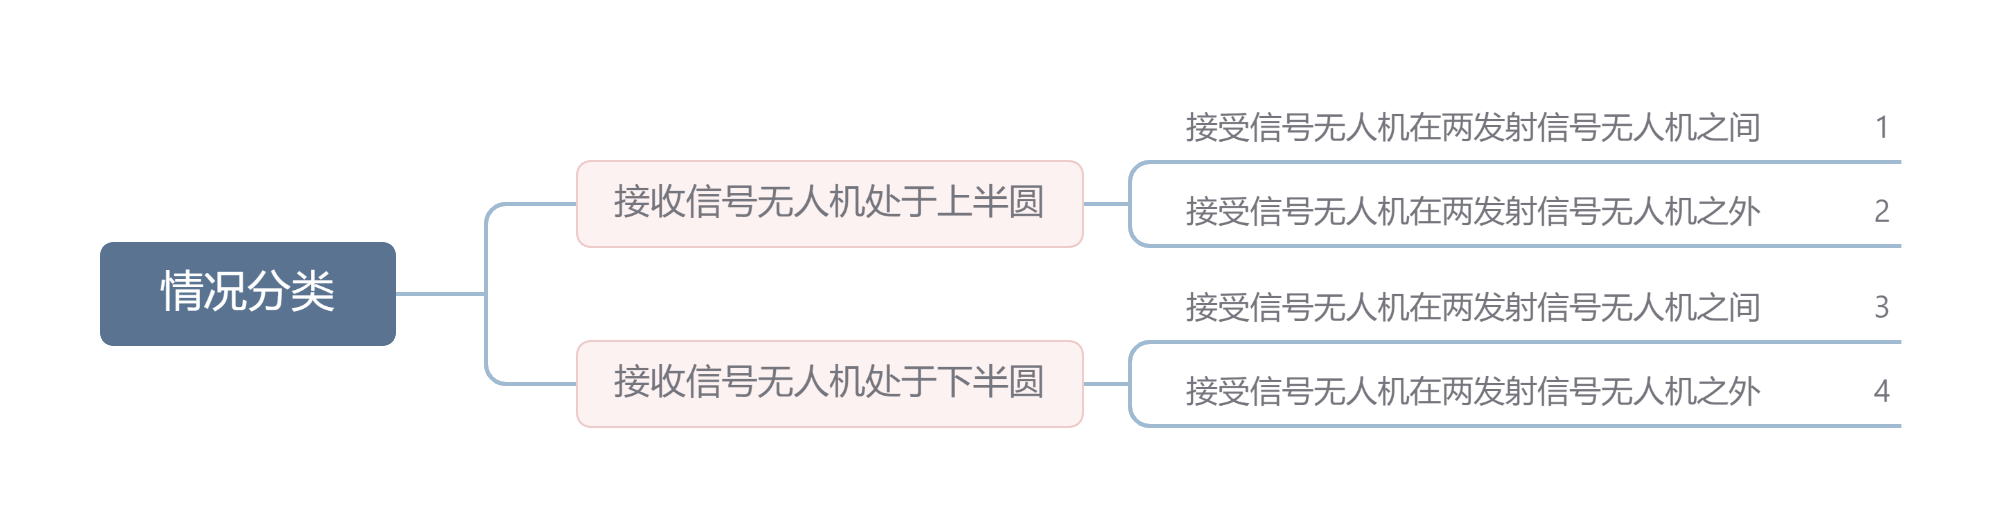
\includegraphics[width=1.0\textwidth]{figures/情况分类.png}
    \caption{问题一第一个任务分类情况}
    \label{fig:classification}
    
\end{figure}


\normalsize

\subsubsection{第一种情况}
第一种情况为接收信号无人机的位于上半圆且接受信号无人机在发射信号无人机中间,具体的示意图如图\ref{fig:case1}所示。

\begin{figure}[H]
    \centering
    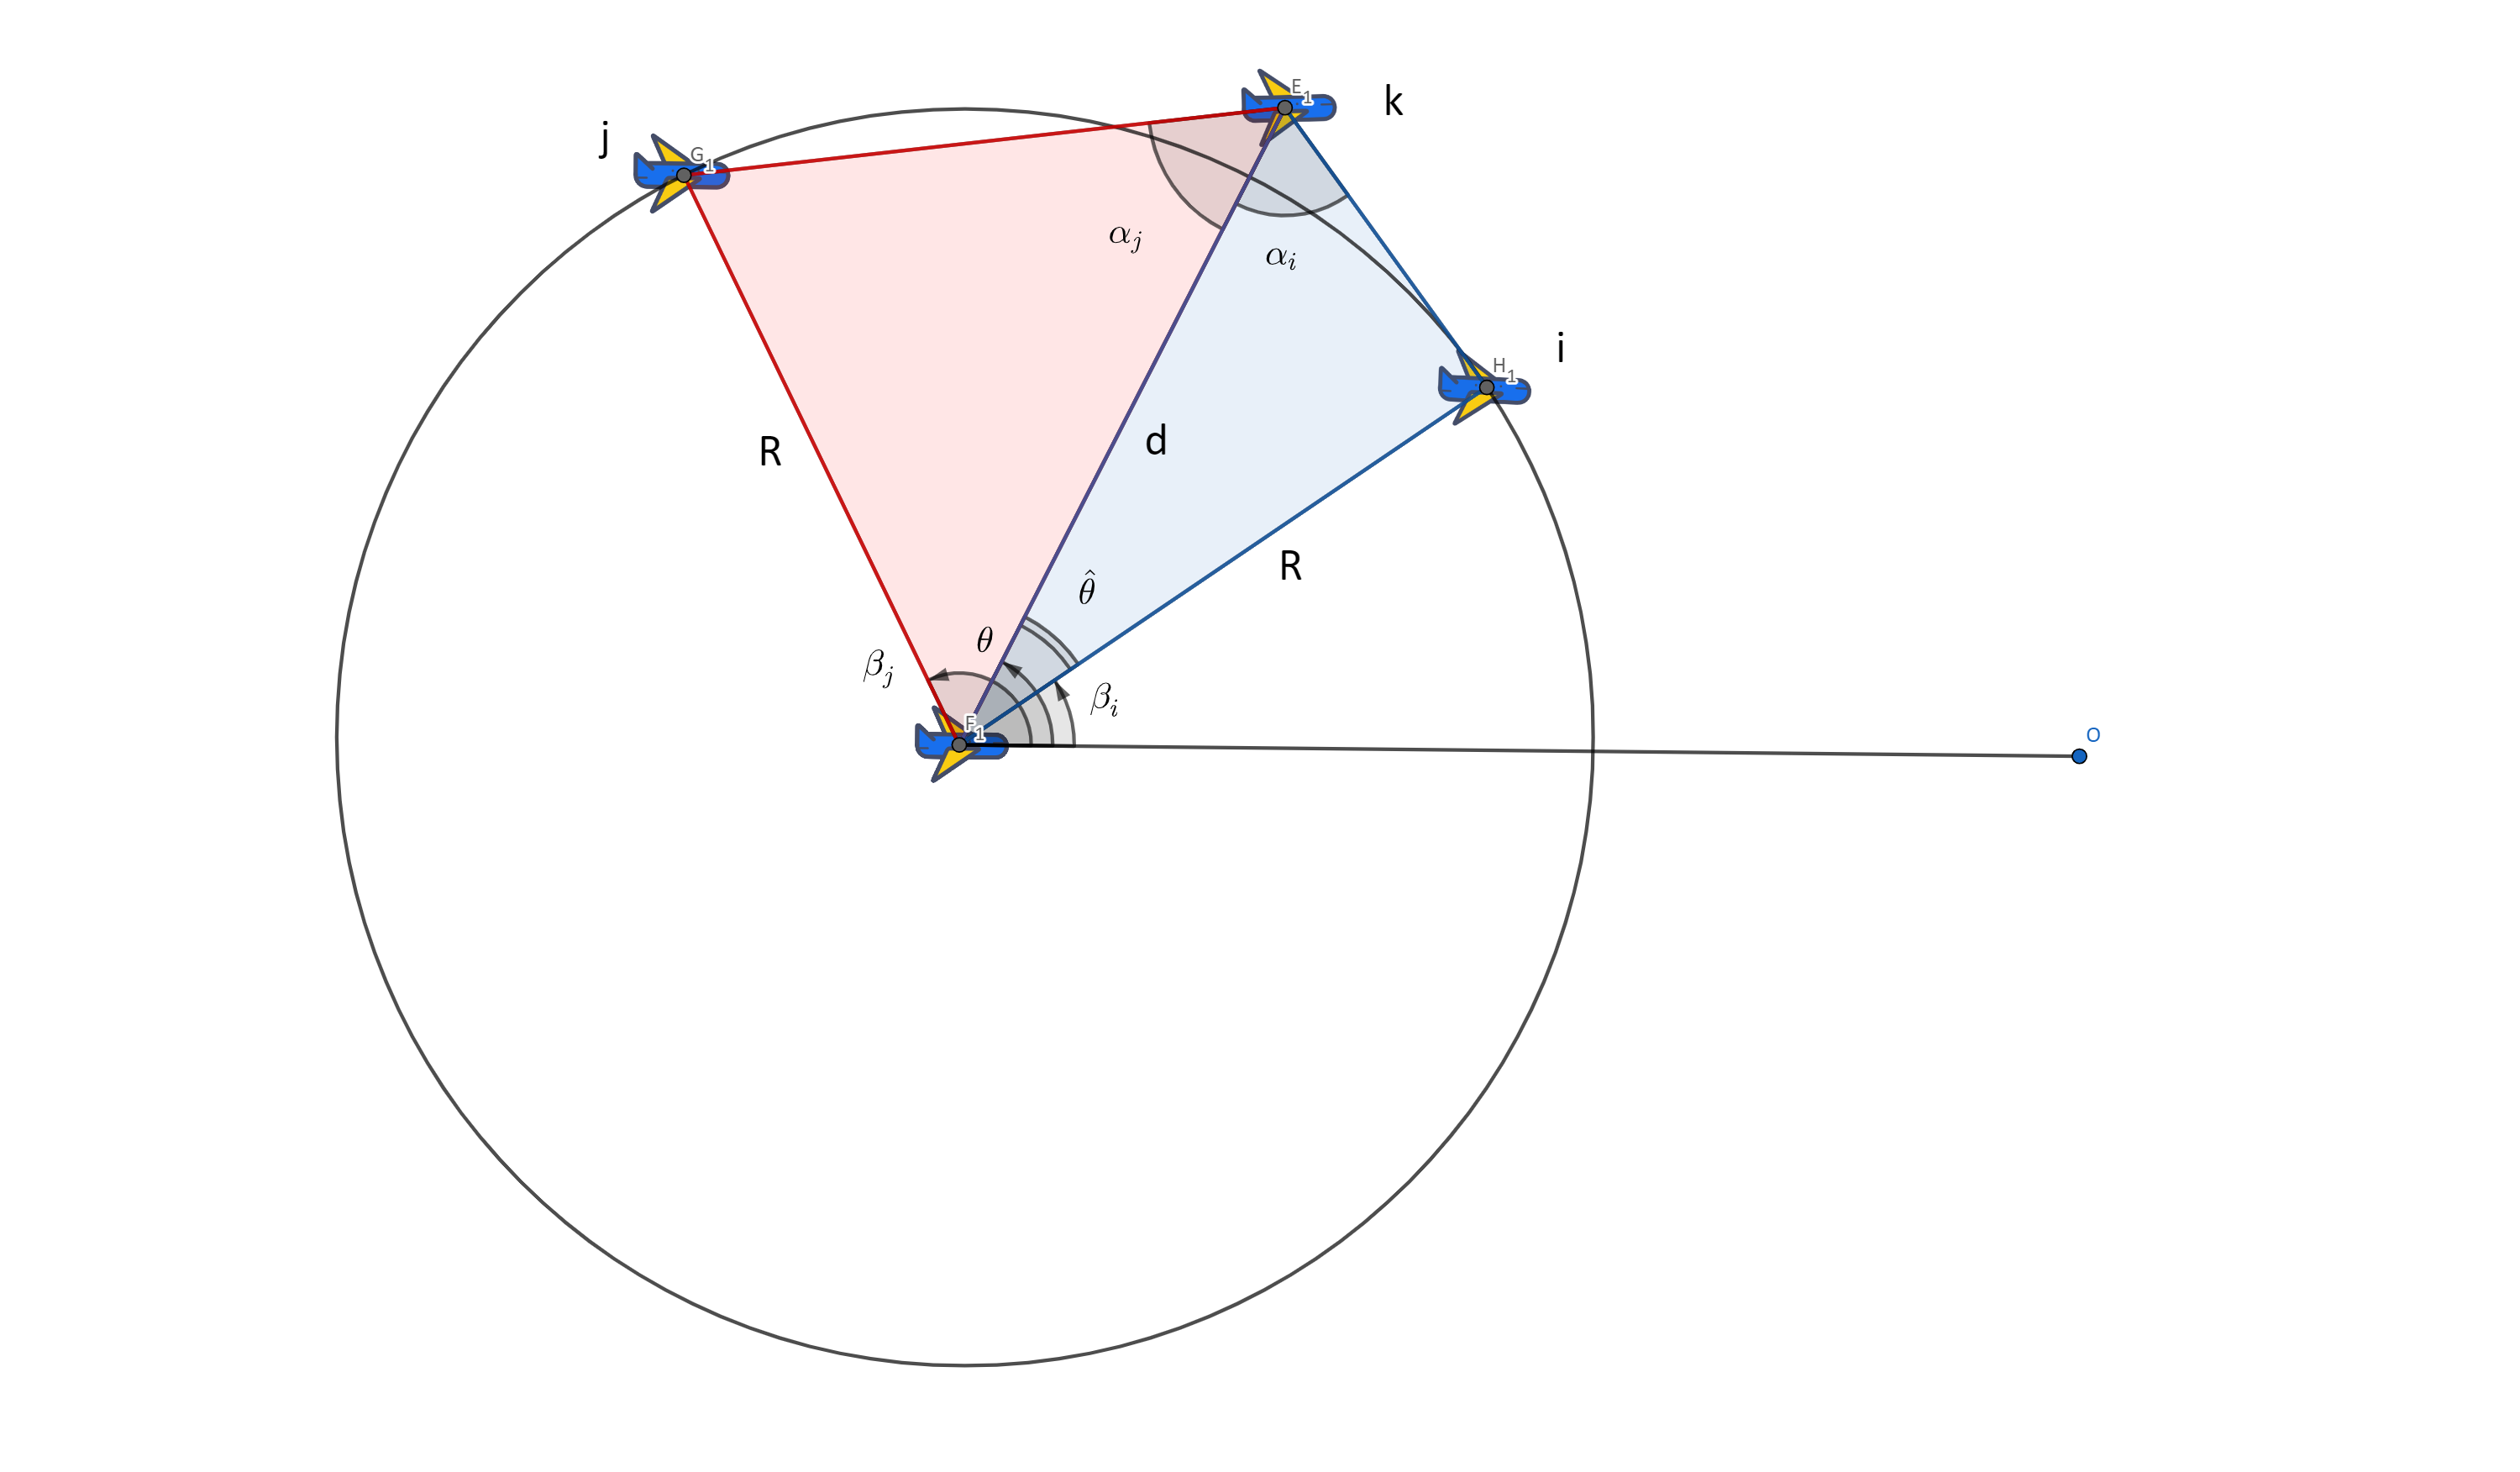
\includegraphics[width=1.0\textwidth]{figures/case 1.png}
    \caption{第一种情况示意图}
    \label{fig:case1}
    
\end{figure}

下面开始分析,对图中两个三角形使用正弦定理,得到的式子如下:
\begin{equation}
\left\{\begin{array}{l}
\frac{d}{\sin \left(\hat{\theta} + \alpha_i\right)}=\frac{R}{\sin \alpha_i} \\
\frac{d}{\sin \left(\beta_j - \beta_i - \hat{\theta} + \alpha_j \right)}=\frac{R}{\sin \alpha_j}
\end{array}\right.
\end{equation}

可以解得对应的解,令 

$$\kappa = \frac{\sin \alpha_i \sin \alpha_j - \sin (\beta_j - \beta_i + \alpha_j) \sin \alpha_i}{\cos \alpha_i \sin \alpha_j + \cos(\beta_j - \beta_i + \alpha_j) \sin \alpha_i}$$

由此得,

$$ 
\hat{\theta}=\left\{
\begin{array}{lcl}
- \arctan \kappa & & {\kappa \leq 0} \\
\pi - \arctan \kappa & & {o.w.}\\
\end{array} \right. 
$$

利用上面得到的数据即可求得坐标,

$$ d = \frac{R \sin(\hat{\theta}+\alpha_i )}{\sin \alpha_i}$$

$$ 
\theta=\left\{
\begin{array}{lcl}
\hat{\theta}+\beta_i & & {\hat{\theta}+\beta_i < 2\pi} \\
\hat{\theta}+\beta_i - 2\pi & & {o.w.}\\
\end{array} \right. 
$$

由上可知可以唯一确定极坐标定位$(d,\theta)$。

\subsubsection{第二种情况}

第二种情况为接收信号无人机的位于上半且接受信号无人机不在发射信号无人机中间,具体的示意图如图\ref{fig:case2}所示。

\begin{figure}[H]
    \centering
    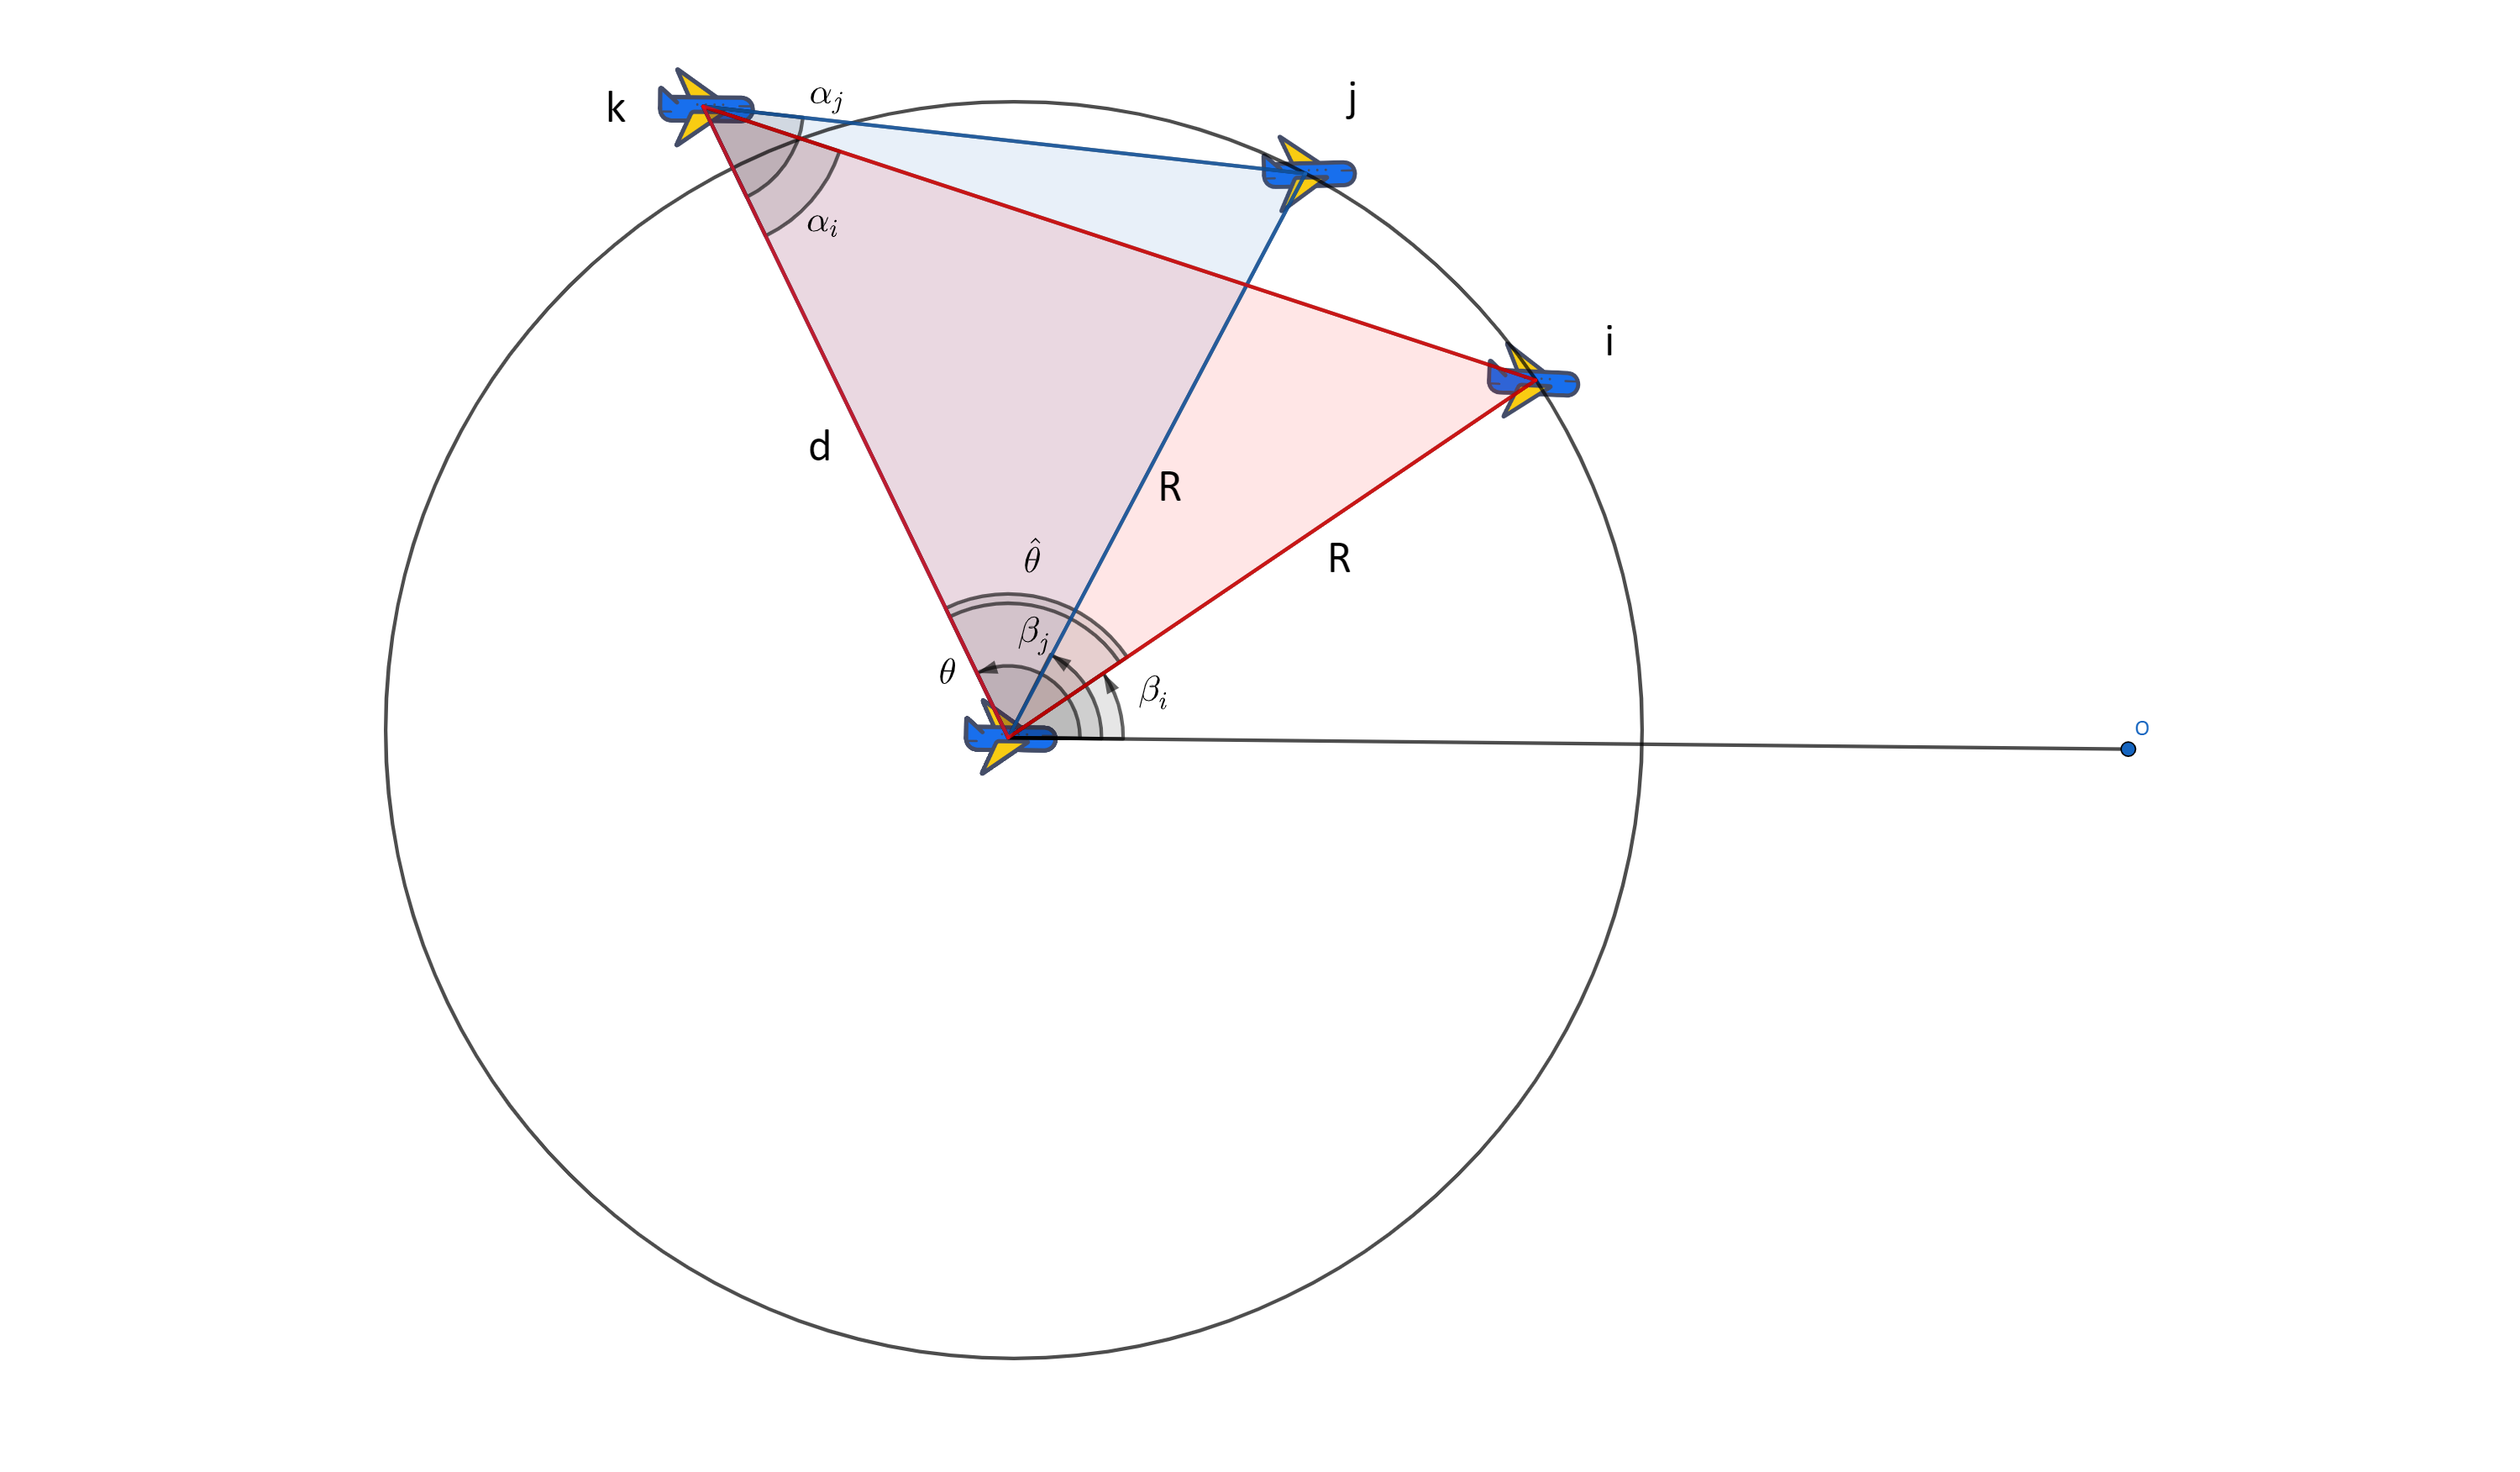
\includegraphics[width=1.0\textwidth]{figures/case 2.png}
    \caption{第二种情况示意图}
    \label{fig:case2}
    
\end{figure}

下面开始分析,对图中两个三角形使用正弦定理,得到的式子如下:
\begin{equation}
\left\{\begin{array}{l}
\frac{d}{\sin \left(\hat{\theta} + \alpha_i\right)}=\frac{R}{\sin \alpha_i} \\
\frac{d}{\sin \left(\hat{\theta}- \beta_j + \beta_i  + \alpha_j \right)}=\frac{R}{\sin \alpha_j}
\end{array}\right.
\end{equation}

可以解得对应的解,令 

$$\kappa_2 = \frac{\sin \alpha_i \sin \alpha_j + \sin (\beta_j - \beta_i - \alpha_j) \sin \alpha_i}{\cos \alpha_i \sin \alpha_j - \cos(\beta_j - \beta_i - \alpha_j) \sin \alpha_i}$$

类似情况一的解法,可以唯一确定极坐标定位$(d,\theta)$。

\subsubsection{第三种情况}
第三种情况为接收信号无人机的位于下半圆且接受信号无人机在发射信号无人机中间,具体的示意图如图\ref{fig:case3}所示。

\begin{figure}[H]
    \centering
    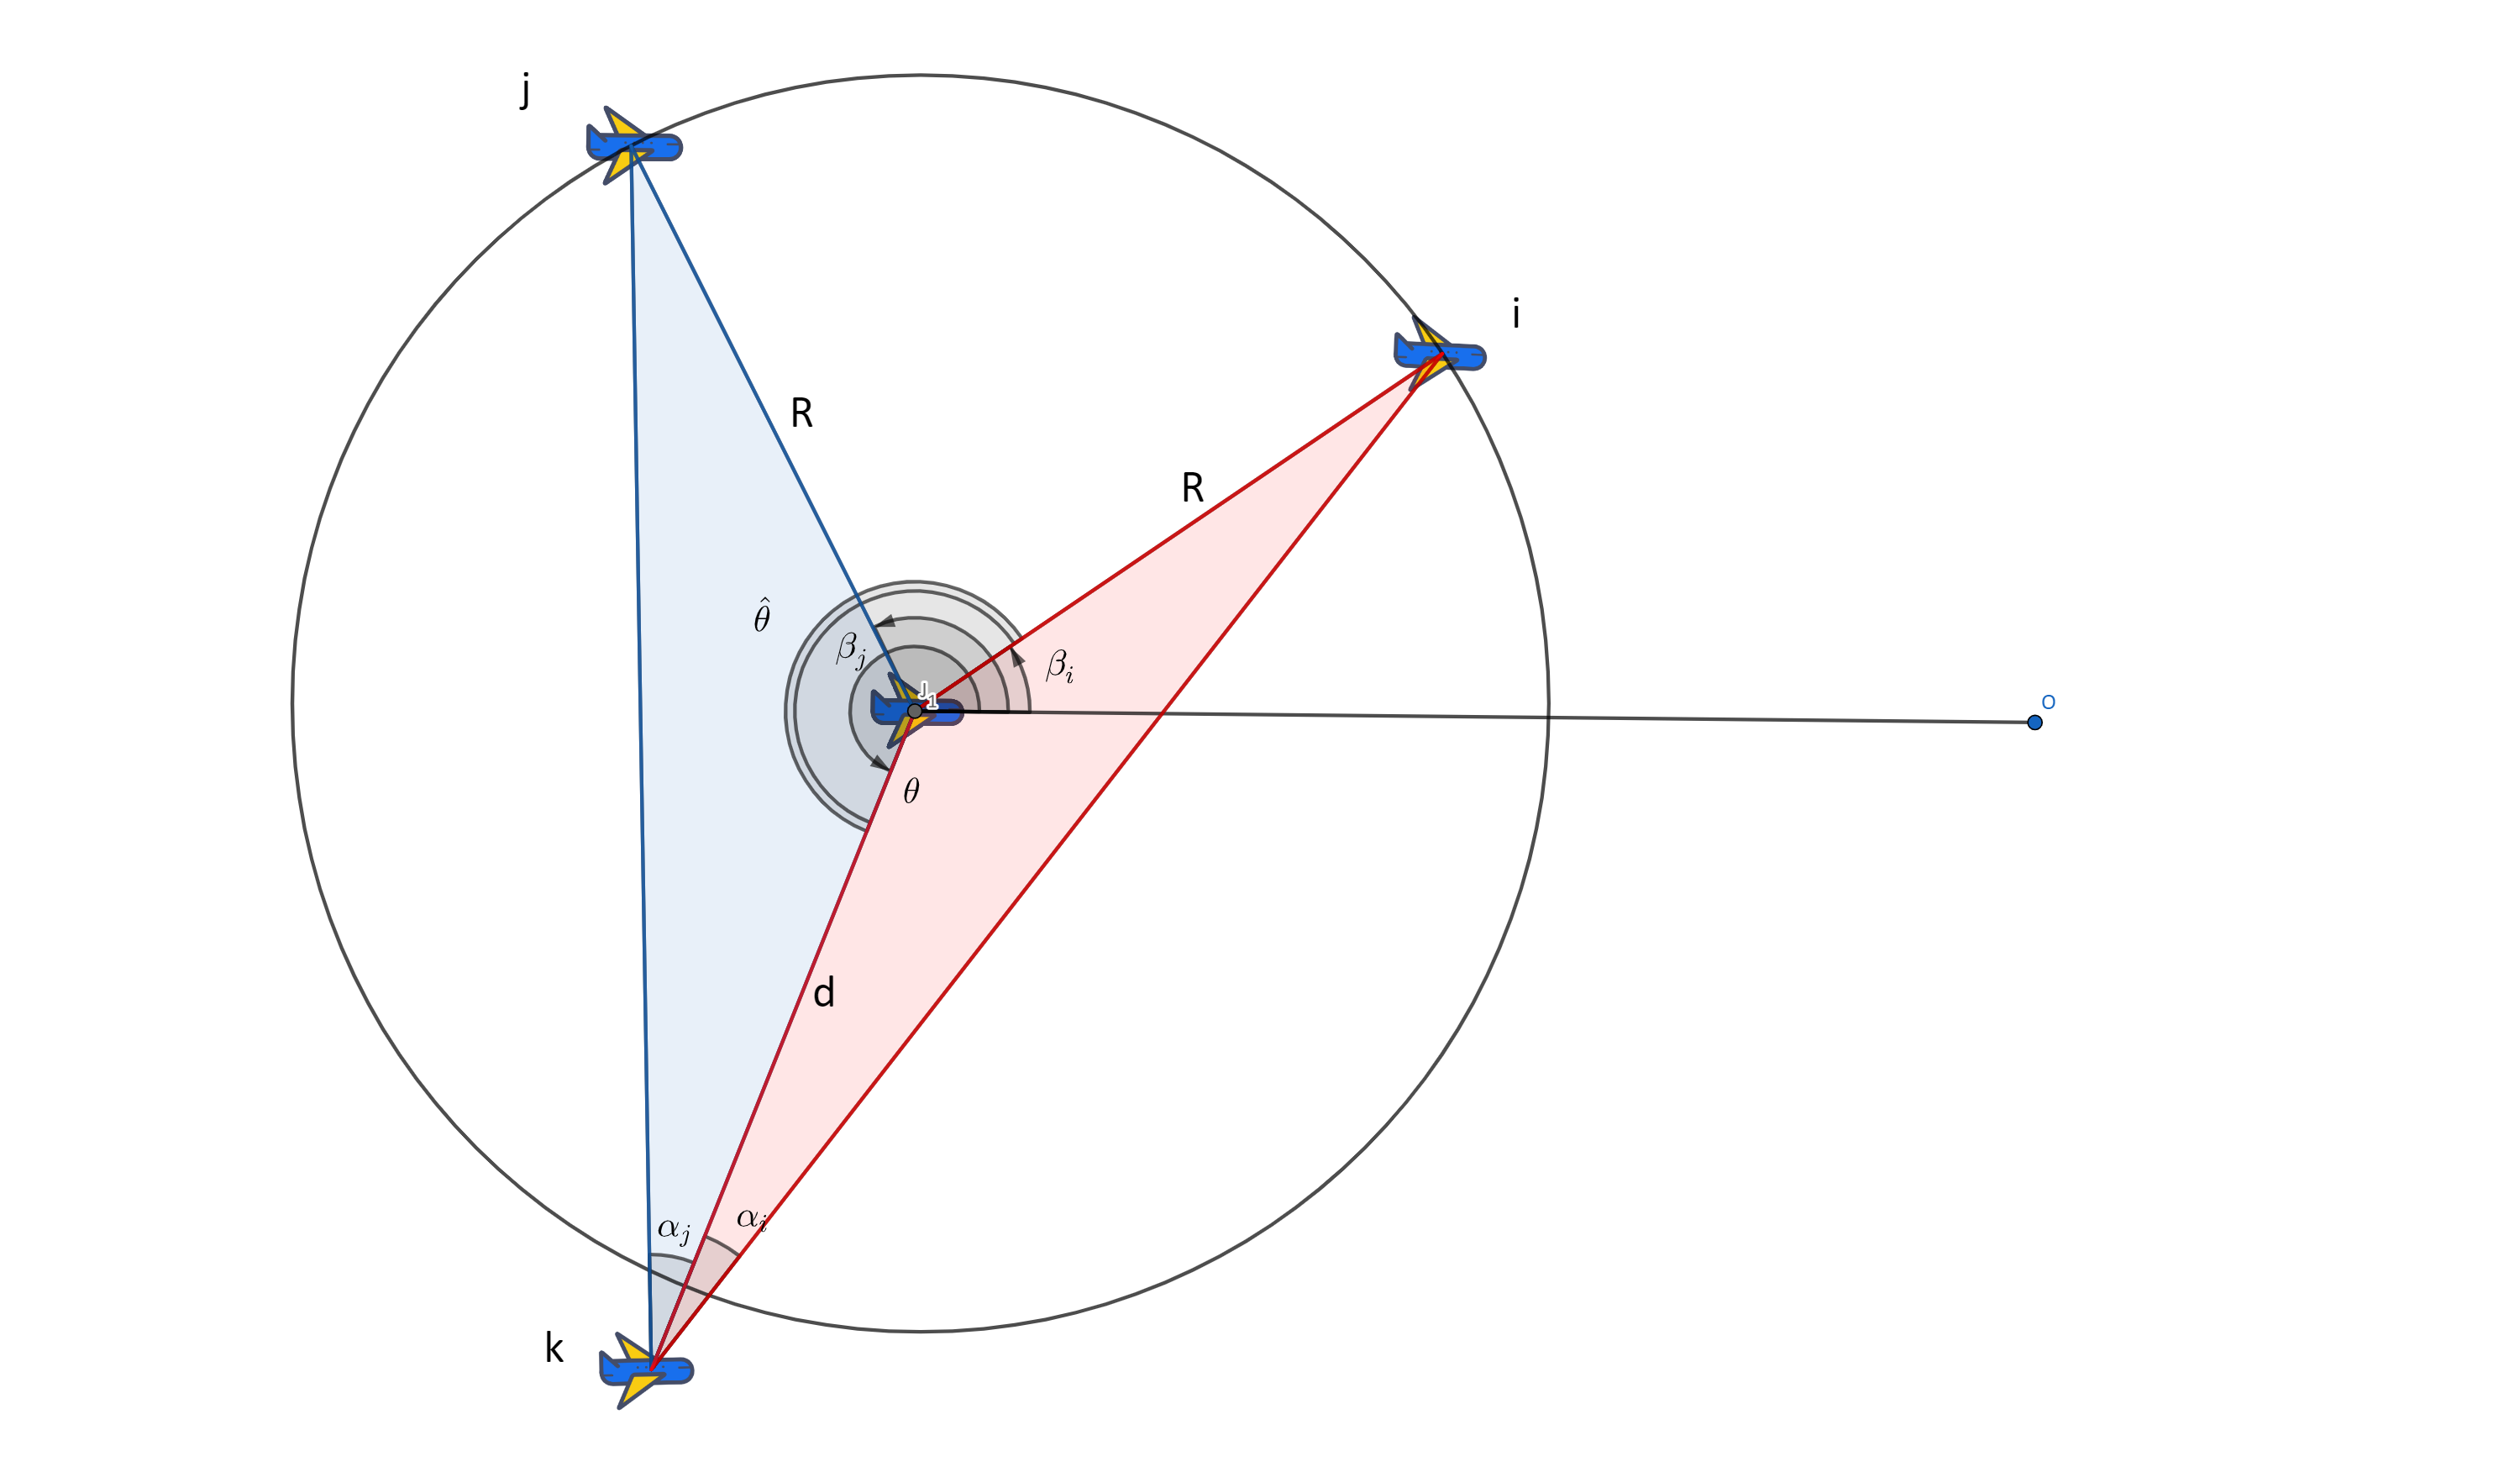
\includegraphics[width=1.0\textwidth]{figures/case 3.png}
    \caption{第三种情况示意图}
    \label{fig:case3}
    
\end{figure}

下面开始分析,对图中两个三角形使用正弦定理,得到的式子如下:
\begin{equation}
\left\{\begin{array}{l}
\frac{d}{\sin \left(-\hat{\theta} + \alpha_i\right)}=\frac{R}{\sin \alpha_i} \\
\frac{d}{\sin \left(\hat{\theta} - \beta_j + \beta_i  + \alpha_j \right)}=\frac{R}{\sin \alpha_j}
\end{array}\right.
\end{equation}

可以解得对应的解,令 

$$\kappa_1 = \frac{\sin \alpha_i \sin \alpha_j - \sin (-\beta_j + \beta_i + \alpha_j) \sin \alpha_i}{-\cos \alpha_i \sin \alpha_j - \cos(-\beta_j + \beta_i + \alpha_j) \sin \alpha_i}$$


由此得,

$$ 
\hat{\theta}=\left\{
\begin{array}{lcl}
\pi + \arctan \kappa & & {\kappa \leq 0} \\
\arctan \kappa & & {o.w.}\\
\end{array} \right. 
$$

利用上面得到的数据即可求得坐标,

$$ d = \frac{R \sin(\hat{\theta}+\alpha_i )}{\sin \alpha_i}$$

$$ 
\theta=\left\{
\begin{array}{lcl}
\beta_i- \hat{\theta}& & {\hat{\theta}+\beta_i < 2\pi} \\
\beta_i- \hat{\theta} +  2\pi & & {o.w.}\\
\end{array} \right. 
$$

由上可知可以唯一确定极坐标定位$(d,\theta)$。


\subsubsection{第四种情况}
第四种情况为接收信号无人机的位于下半圆且接受信号无人机在发射信号无人机中间,具体的示意图如图\ref{fig:case4}所示。

\begin{figure}[H]
    \centering
    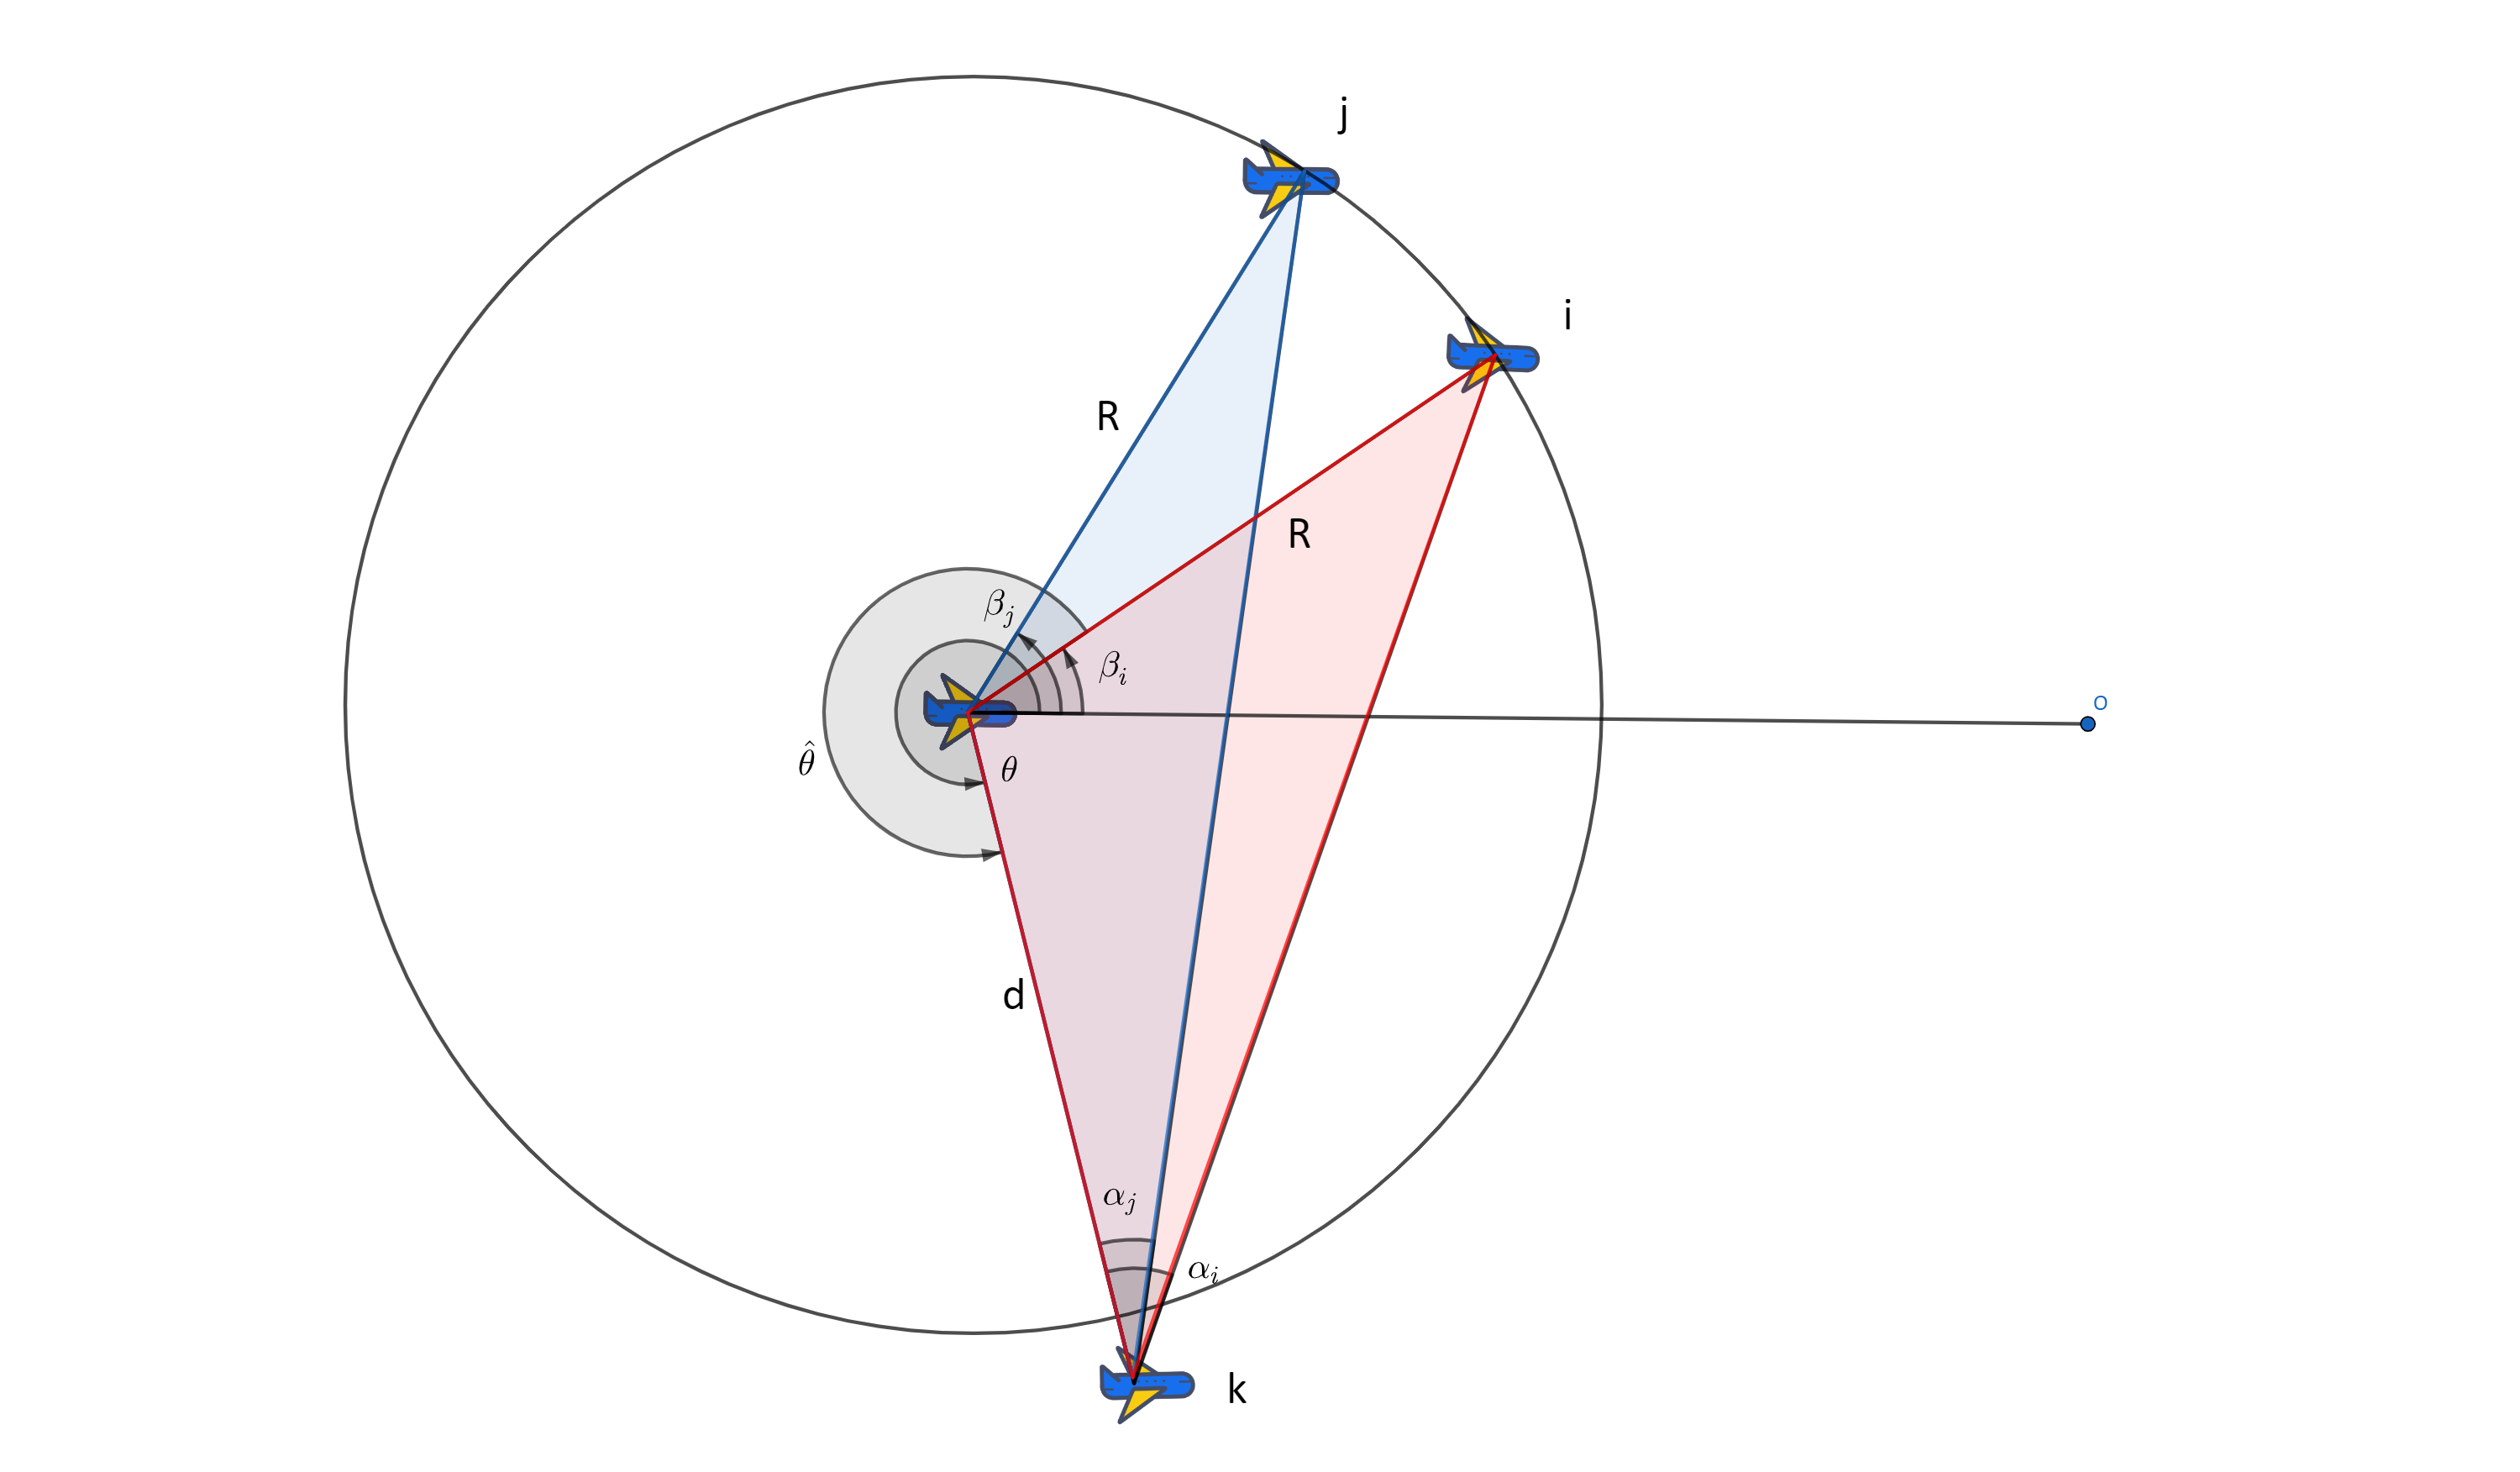
\includegraphics[width=1.0\textwidth]{figures/case 4.png}
    \caption{第四种情况示意图}
    \label{fig:case4}
    
\end{figure}


对图中两个三角形使用正弦定理,得到的式子如下:
\begin{equation}
\left\{\begin{array}{l}
\frac{d}{\sin \left(-\hat{\theta} + \alpha_i\right)}=\frac{R}{\sin \alpha_i} \\
\frac{d}{\sin \left(\beta_j - \beta_i  -\hat{\theta}  + \alpha_j \right)}=\frac{R}{\sin \alpha_j}
\end{array}\right.
\end{equation}

可以解得对应的解,令 

$$\kappa_1 = \frac{\sin \alpha_i \sin \alpha_j - \sin (\beta_j - \beta_i + \alpha_j) \sin \alpha_i}{-\cos \alpha_i \sin \alpha_j + \cos(\beta_j - \beta_i + \alpha_j) \sin \alpha_i}$$

类似情况三的解法,可以唯一确定极坐标定位$(d,\theta)$。

综上所述,针对不同无人机的相对位置的情况,都可以唯一确定极坐标,从而实现有效定位。

\subsection{第二个任务——确定最少无人机架数实现有效定位}

第二个任务要求当发射信号无人机编号未知时,确定实现有效定位所需最少的无人机架数。事实上,所需发射信号无人机的数量和接收信号无人机的最大可能偏离程度有关。根据接收信号无人机的不同偏离程度,可以分为以下两种情形。

\subsubsection{情形一}

当接收信号的无人机偏差总是在很小范围内,或该无人机始终在圆周上时,还需一架无人机发射信号即可实现有效定位。
设接收信号的无人机的编号为$k$,发射信号的无人机的编号为$x$($x$未知),示意图如图\ref{fig:pos1}所示。

\begin{figure}[H]
    \centering
    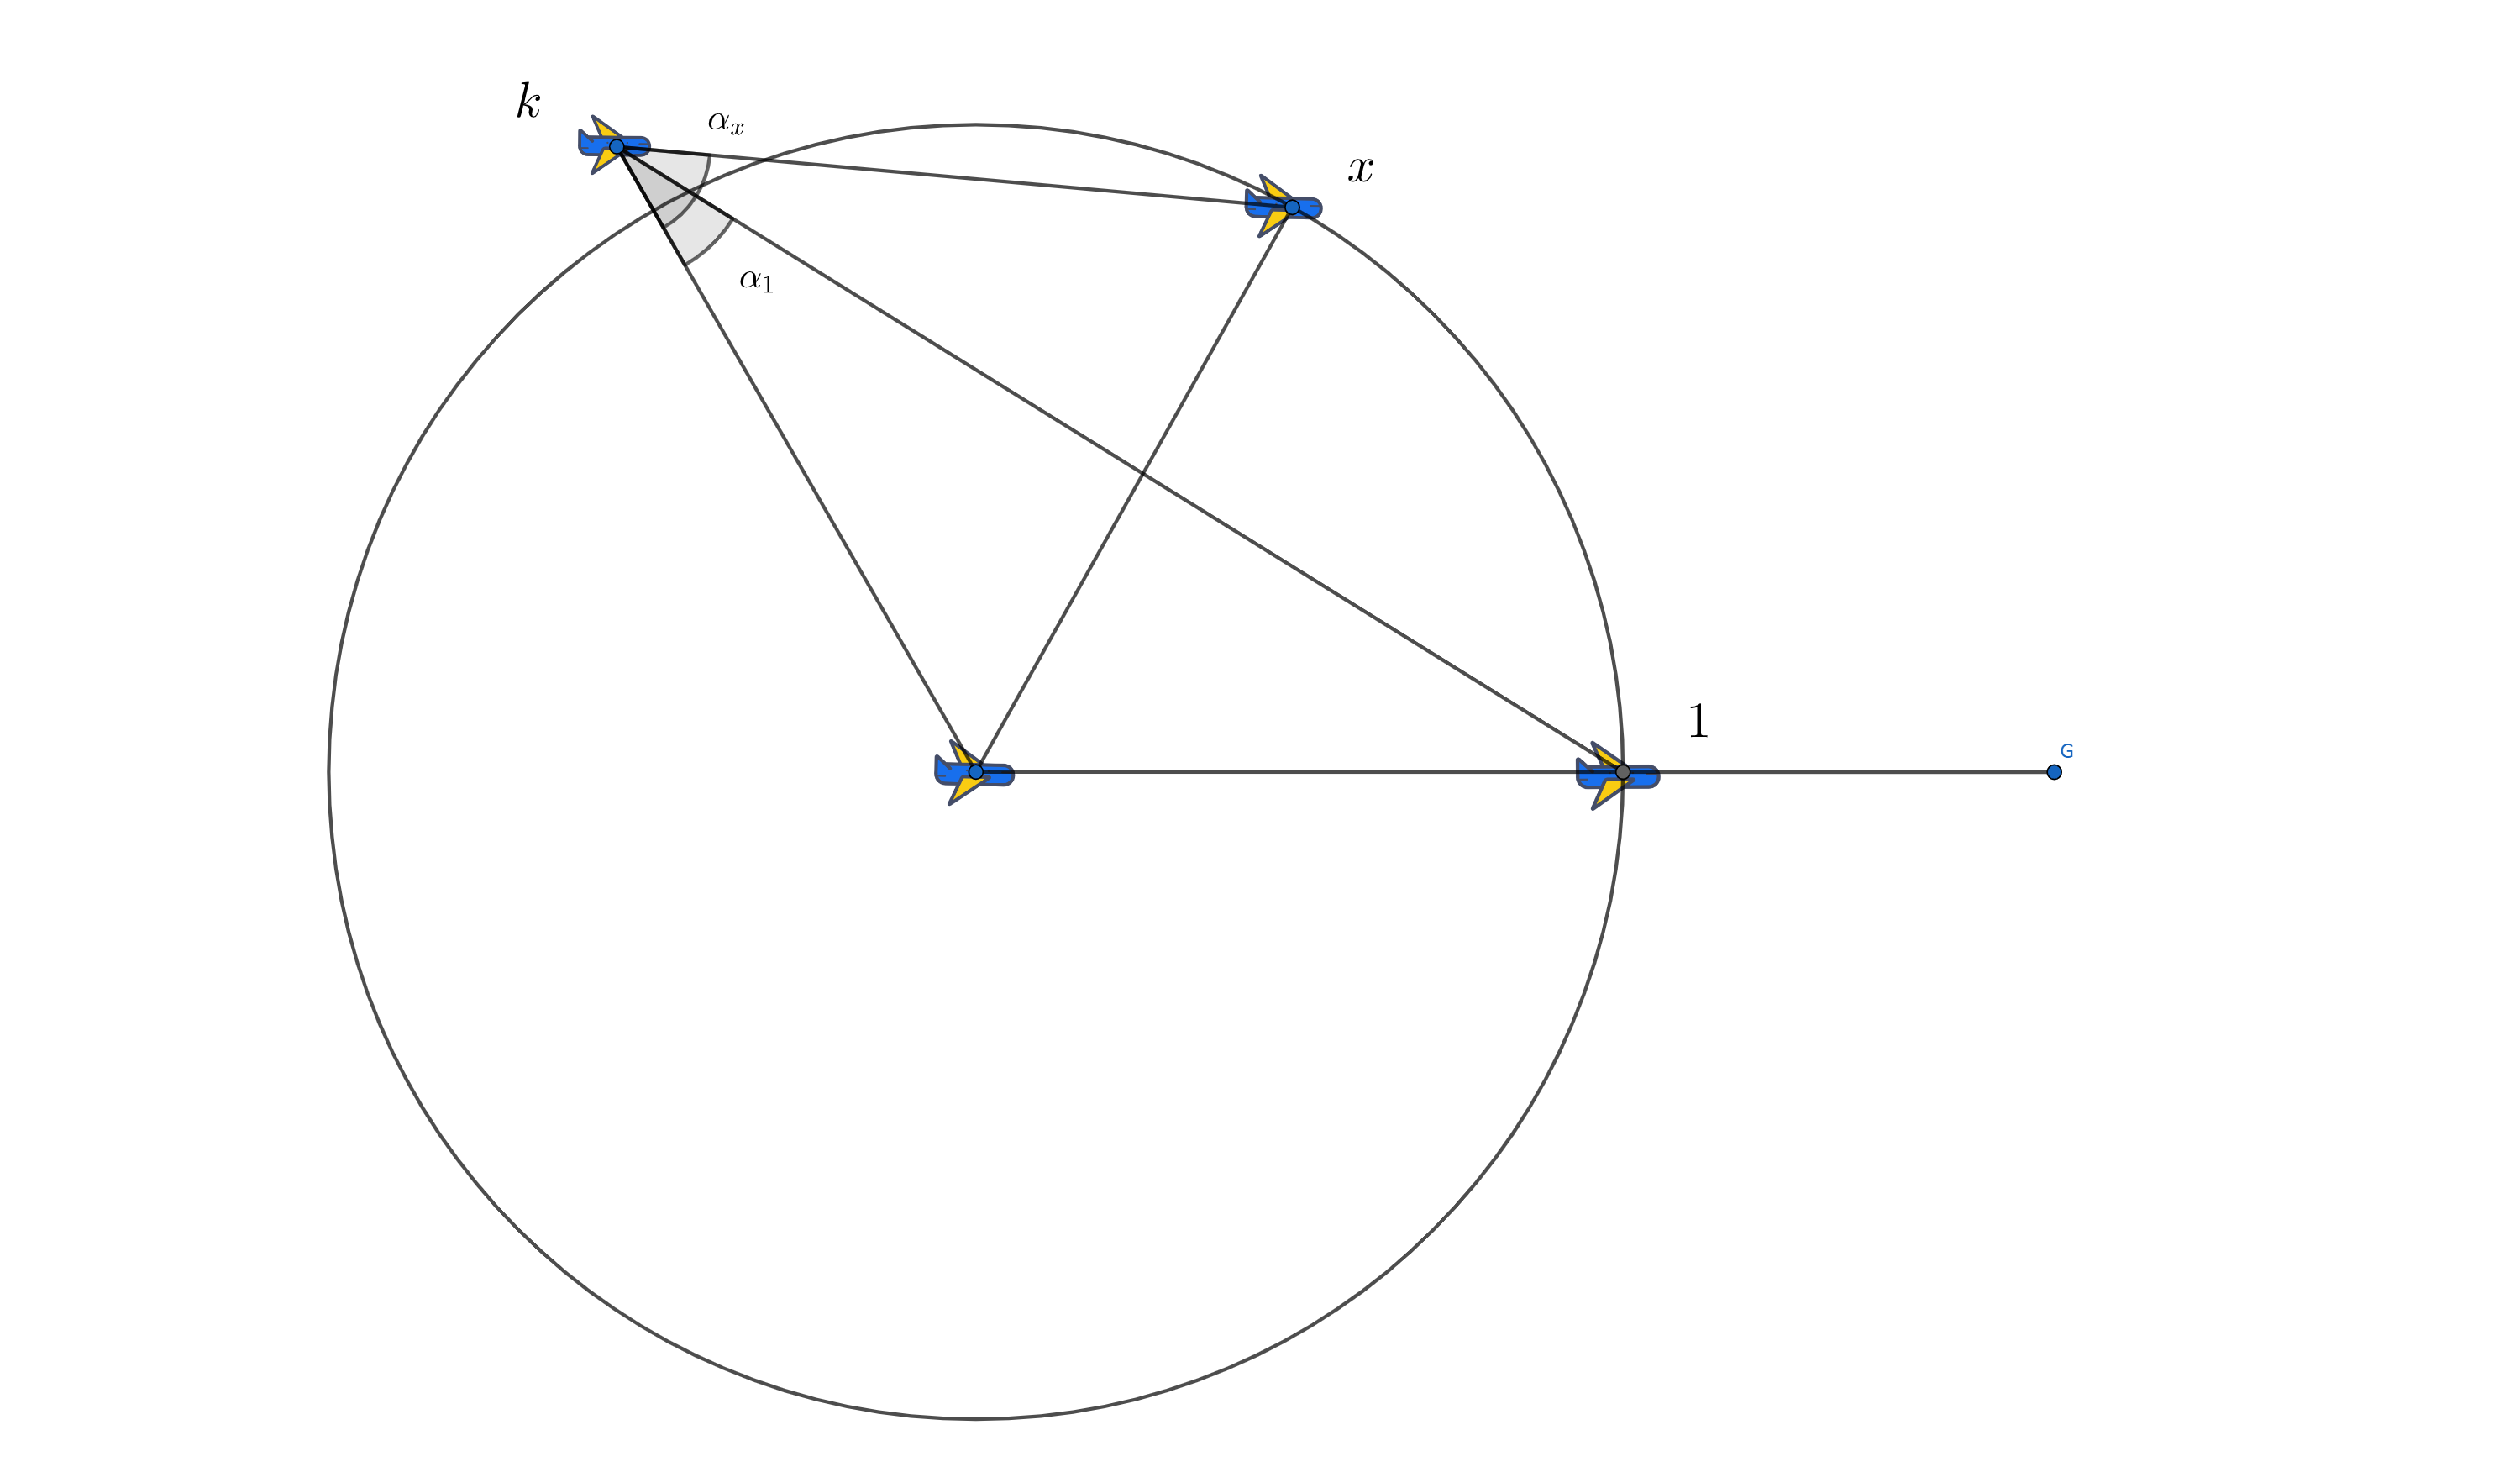
\includegraphics[width=1.0\textwidth]{figures/T2 fig0.png}
    \caption{情形一示意图}
    \label{fig:pos1}
\end{figure}


考虑编号$x$和已知三个角间的关联,注意到在这种情况下,无人机$1,k,x$所成角
$\alpha_3$近似于弧所对圆周角。
若$k\le5$,则当且仅当$\alpha_x$为接收角度信号中的最大角时,
$2 \leq x \leq k-1$,此时$\alpha_3\approx0.5 \cdot \frac{2}{9}\pi \cdot(x-1) $,从而可以由$\alpha_3$确定$x$的值。当$\alpha_x$不为接收角度信号中的最大角时,$\alpha_3\approx0.5 \cdot \frac{2}{9}\pi \cdot(10-x) $,$x$的值也可以唯一确定。
同理可知$k\geq6$时,也可以运用给定角的关系锁定发射信号无人机的编号。

综上所述,在这类情形中,三个角的关系足以确定发射信号无人机的编号,从而可以将问题转化为第一个任务,进而实现无人机的有效定位。

\subsubsection{情形二}

当接受信号的无人机可能偏离圆周且偏差较为显著时,还需要两架无人机发射信号才可实现有效定位。

\begin{figure}[H]
    \centering
    \begin{minipage}[c]{0.9\textwidth}
        \centering
        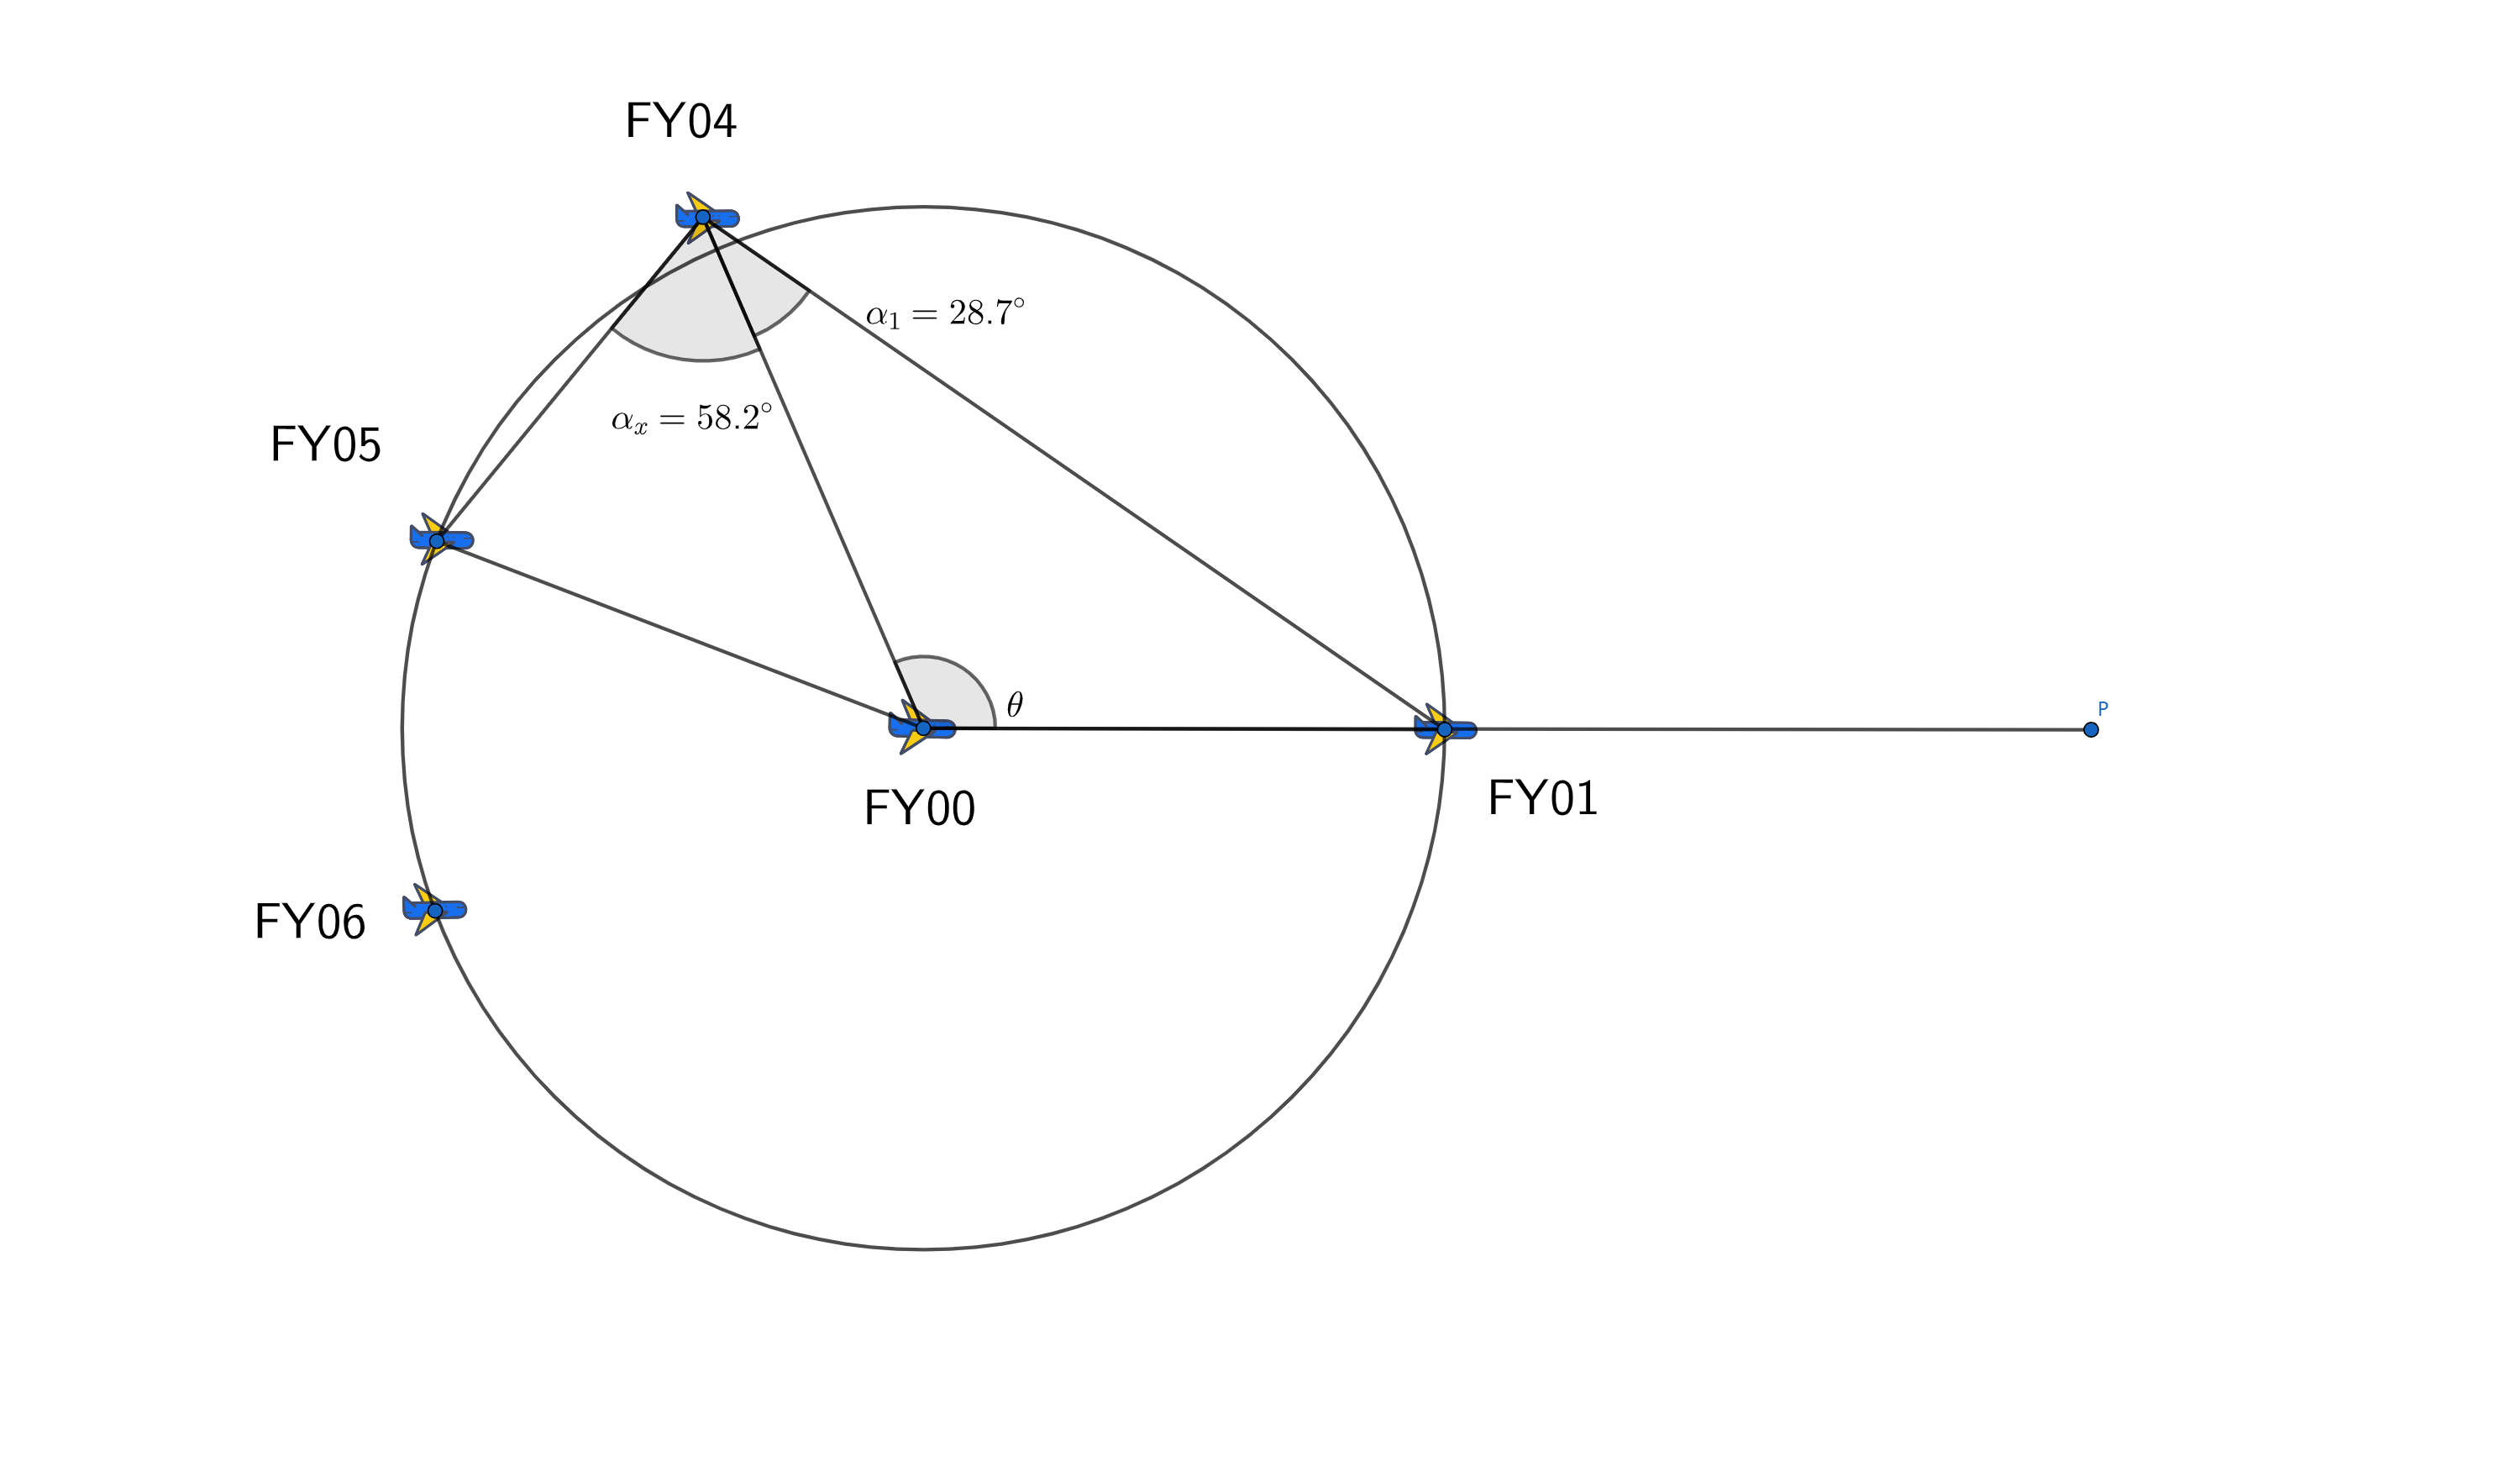
\includegraphics[width=0.95\textwidth]{figures/T2 fig1.png}
        \subcaption{01,05发射,04接收}
        \label{fig:sample-figure-a}
    \end{minipage}
    \begin{minipage}[c]{0.95\textwidth}
        \centering
        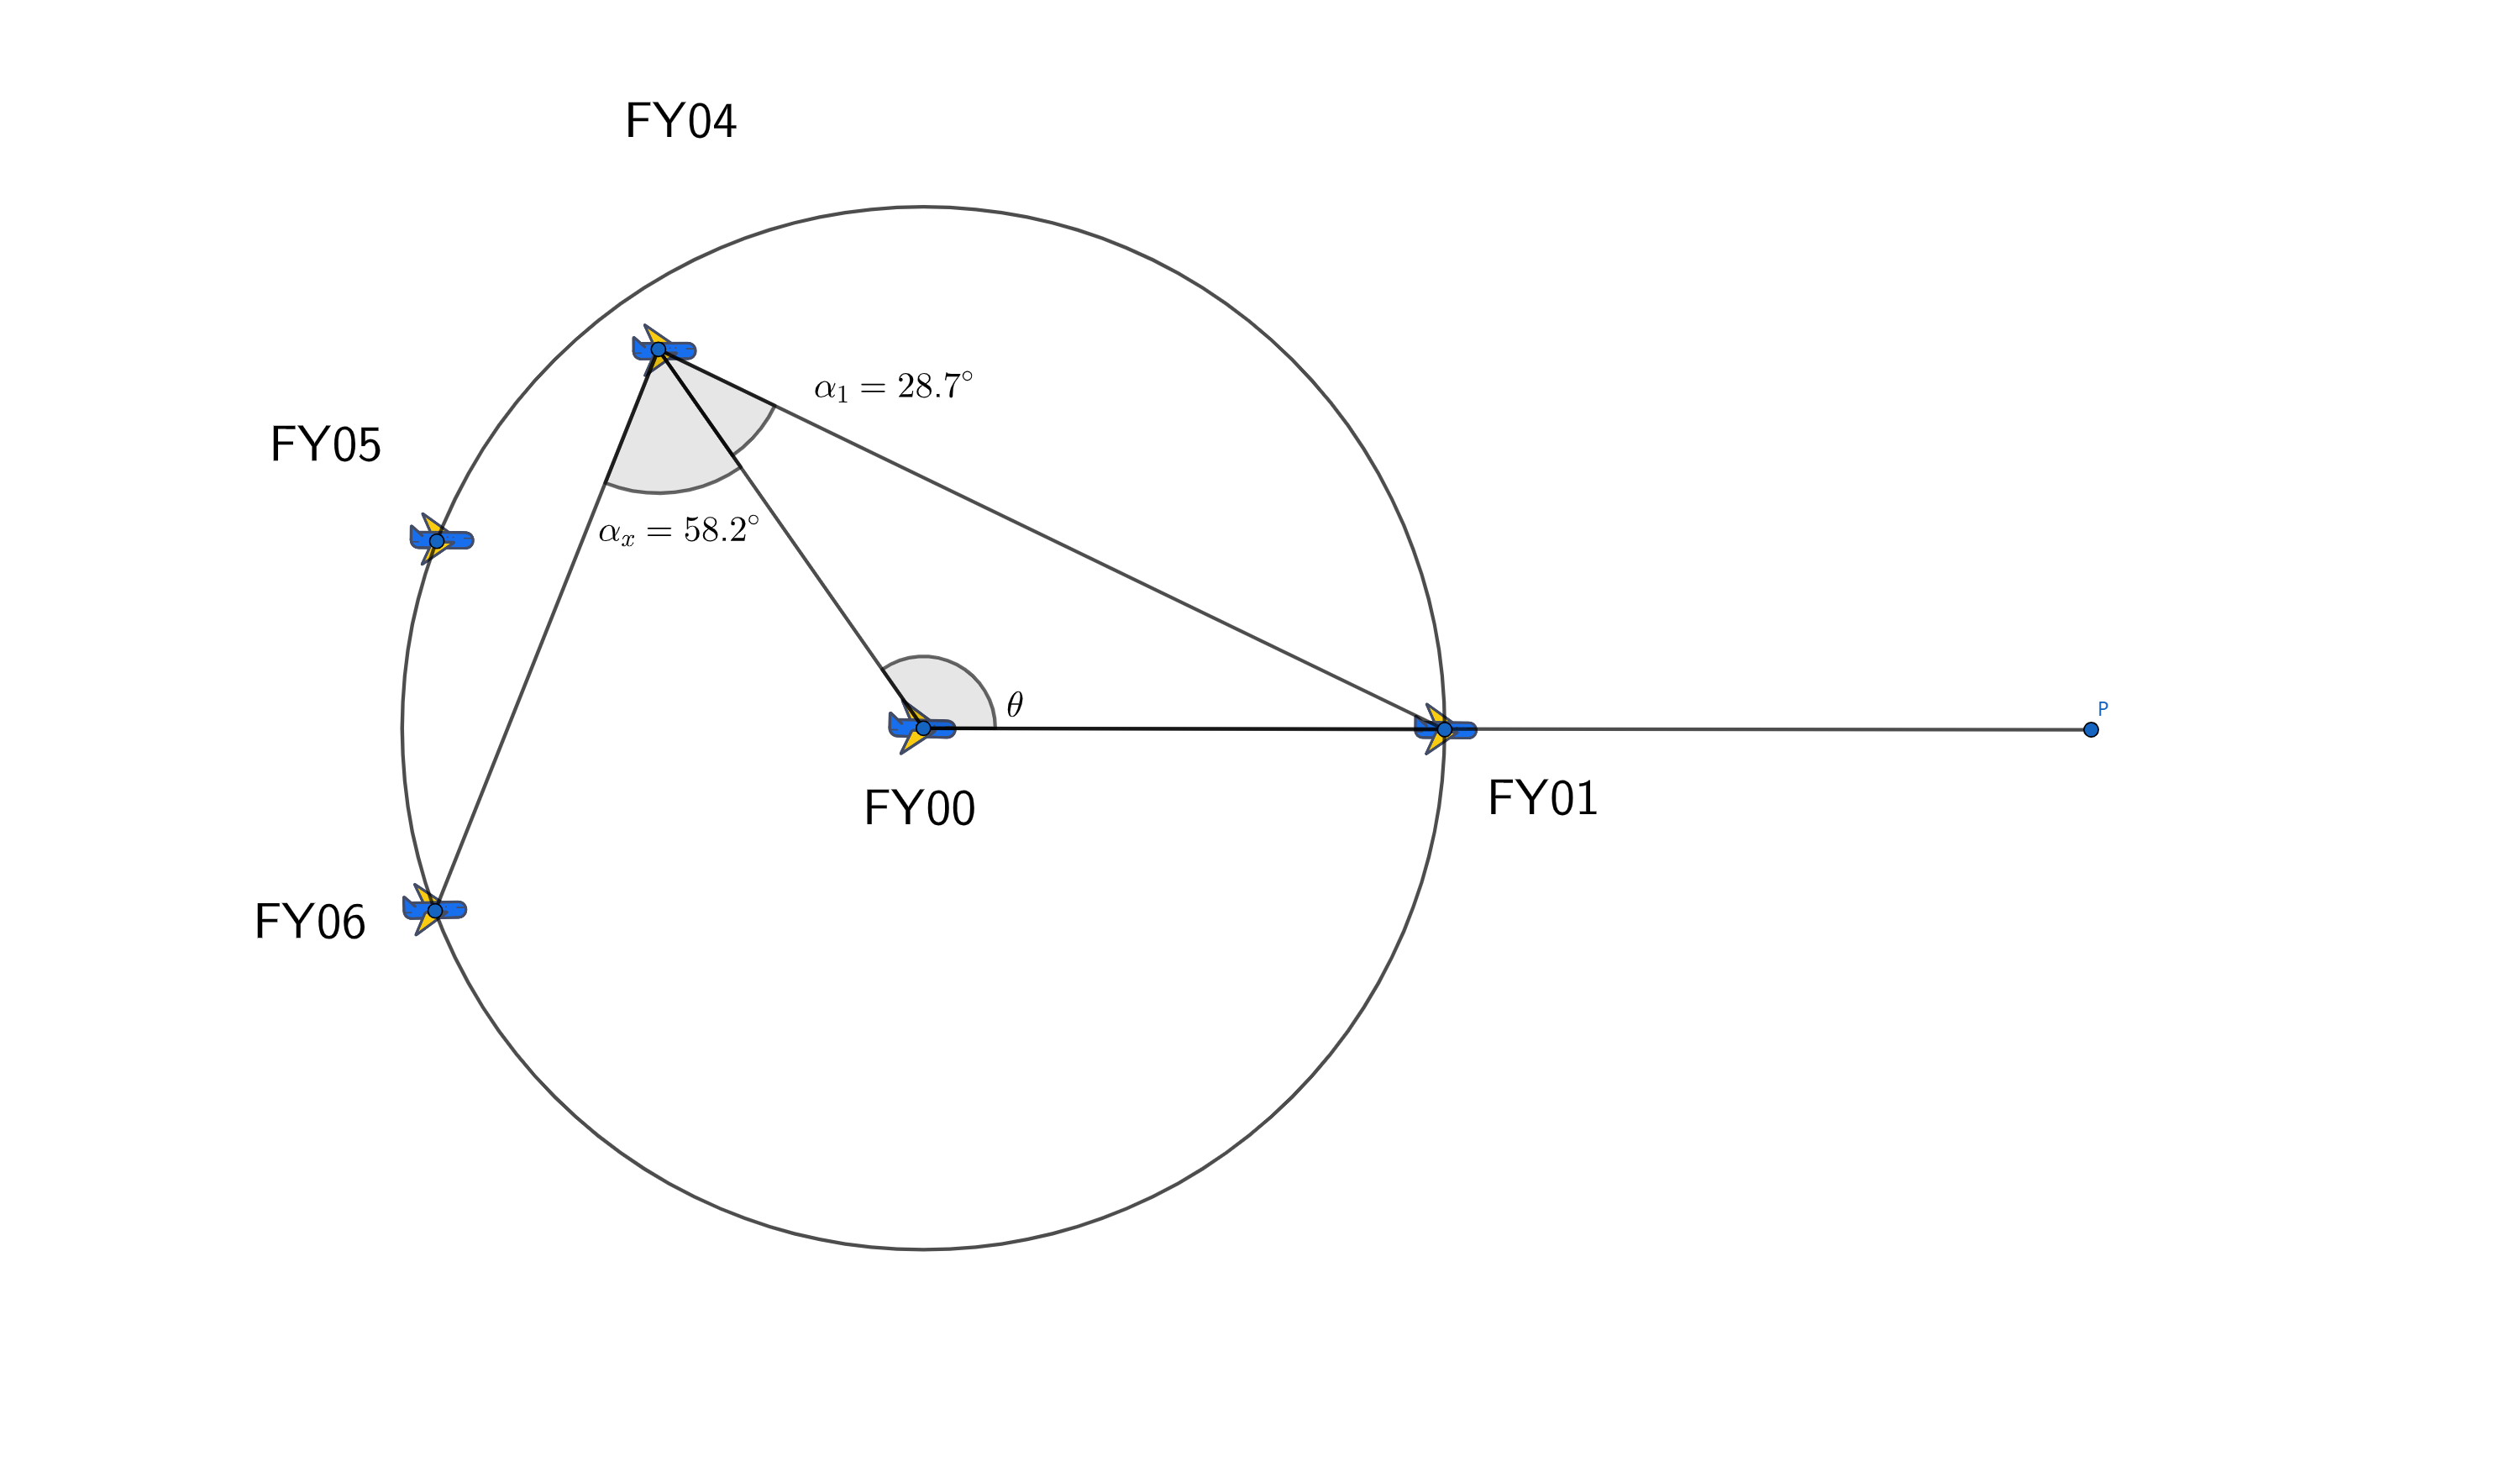
\includegraphics[width=0.95\textwidth]{figures/T2 fig2.png}
        \subcaption{01,06发射,04接收}
        \label{fig:sample-figure-b}
    \end{minipage}
    \caption{情形二仅添加一架无人机产生错误定位示意图}
    \label{fig:comparison}
\end{figure}

如图\ref{fig:comparison}所示,若此时仅用一架无人机发射信号,在已知角度信息下可能无法区分发射信号无人机的编号,导致错误的定位。\\

以下证明用两架无人机发射信号可以实现有效定位。设发射信号的无人机编号为$x,y$。显然,可以通过6个已知角的信息,唯一确定两架发射信号无人机的相对位置关系,这里先考虑其中的一种情形,示意图如图\ref{fig:pos2}所示。\\

\begin{figure}[H]
    \centering
    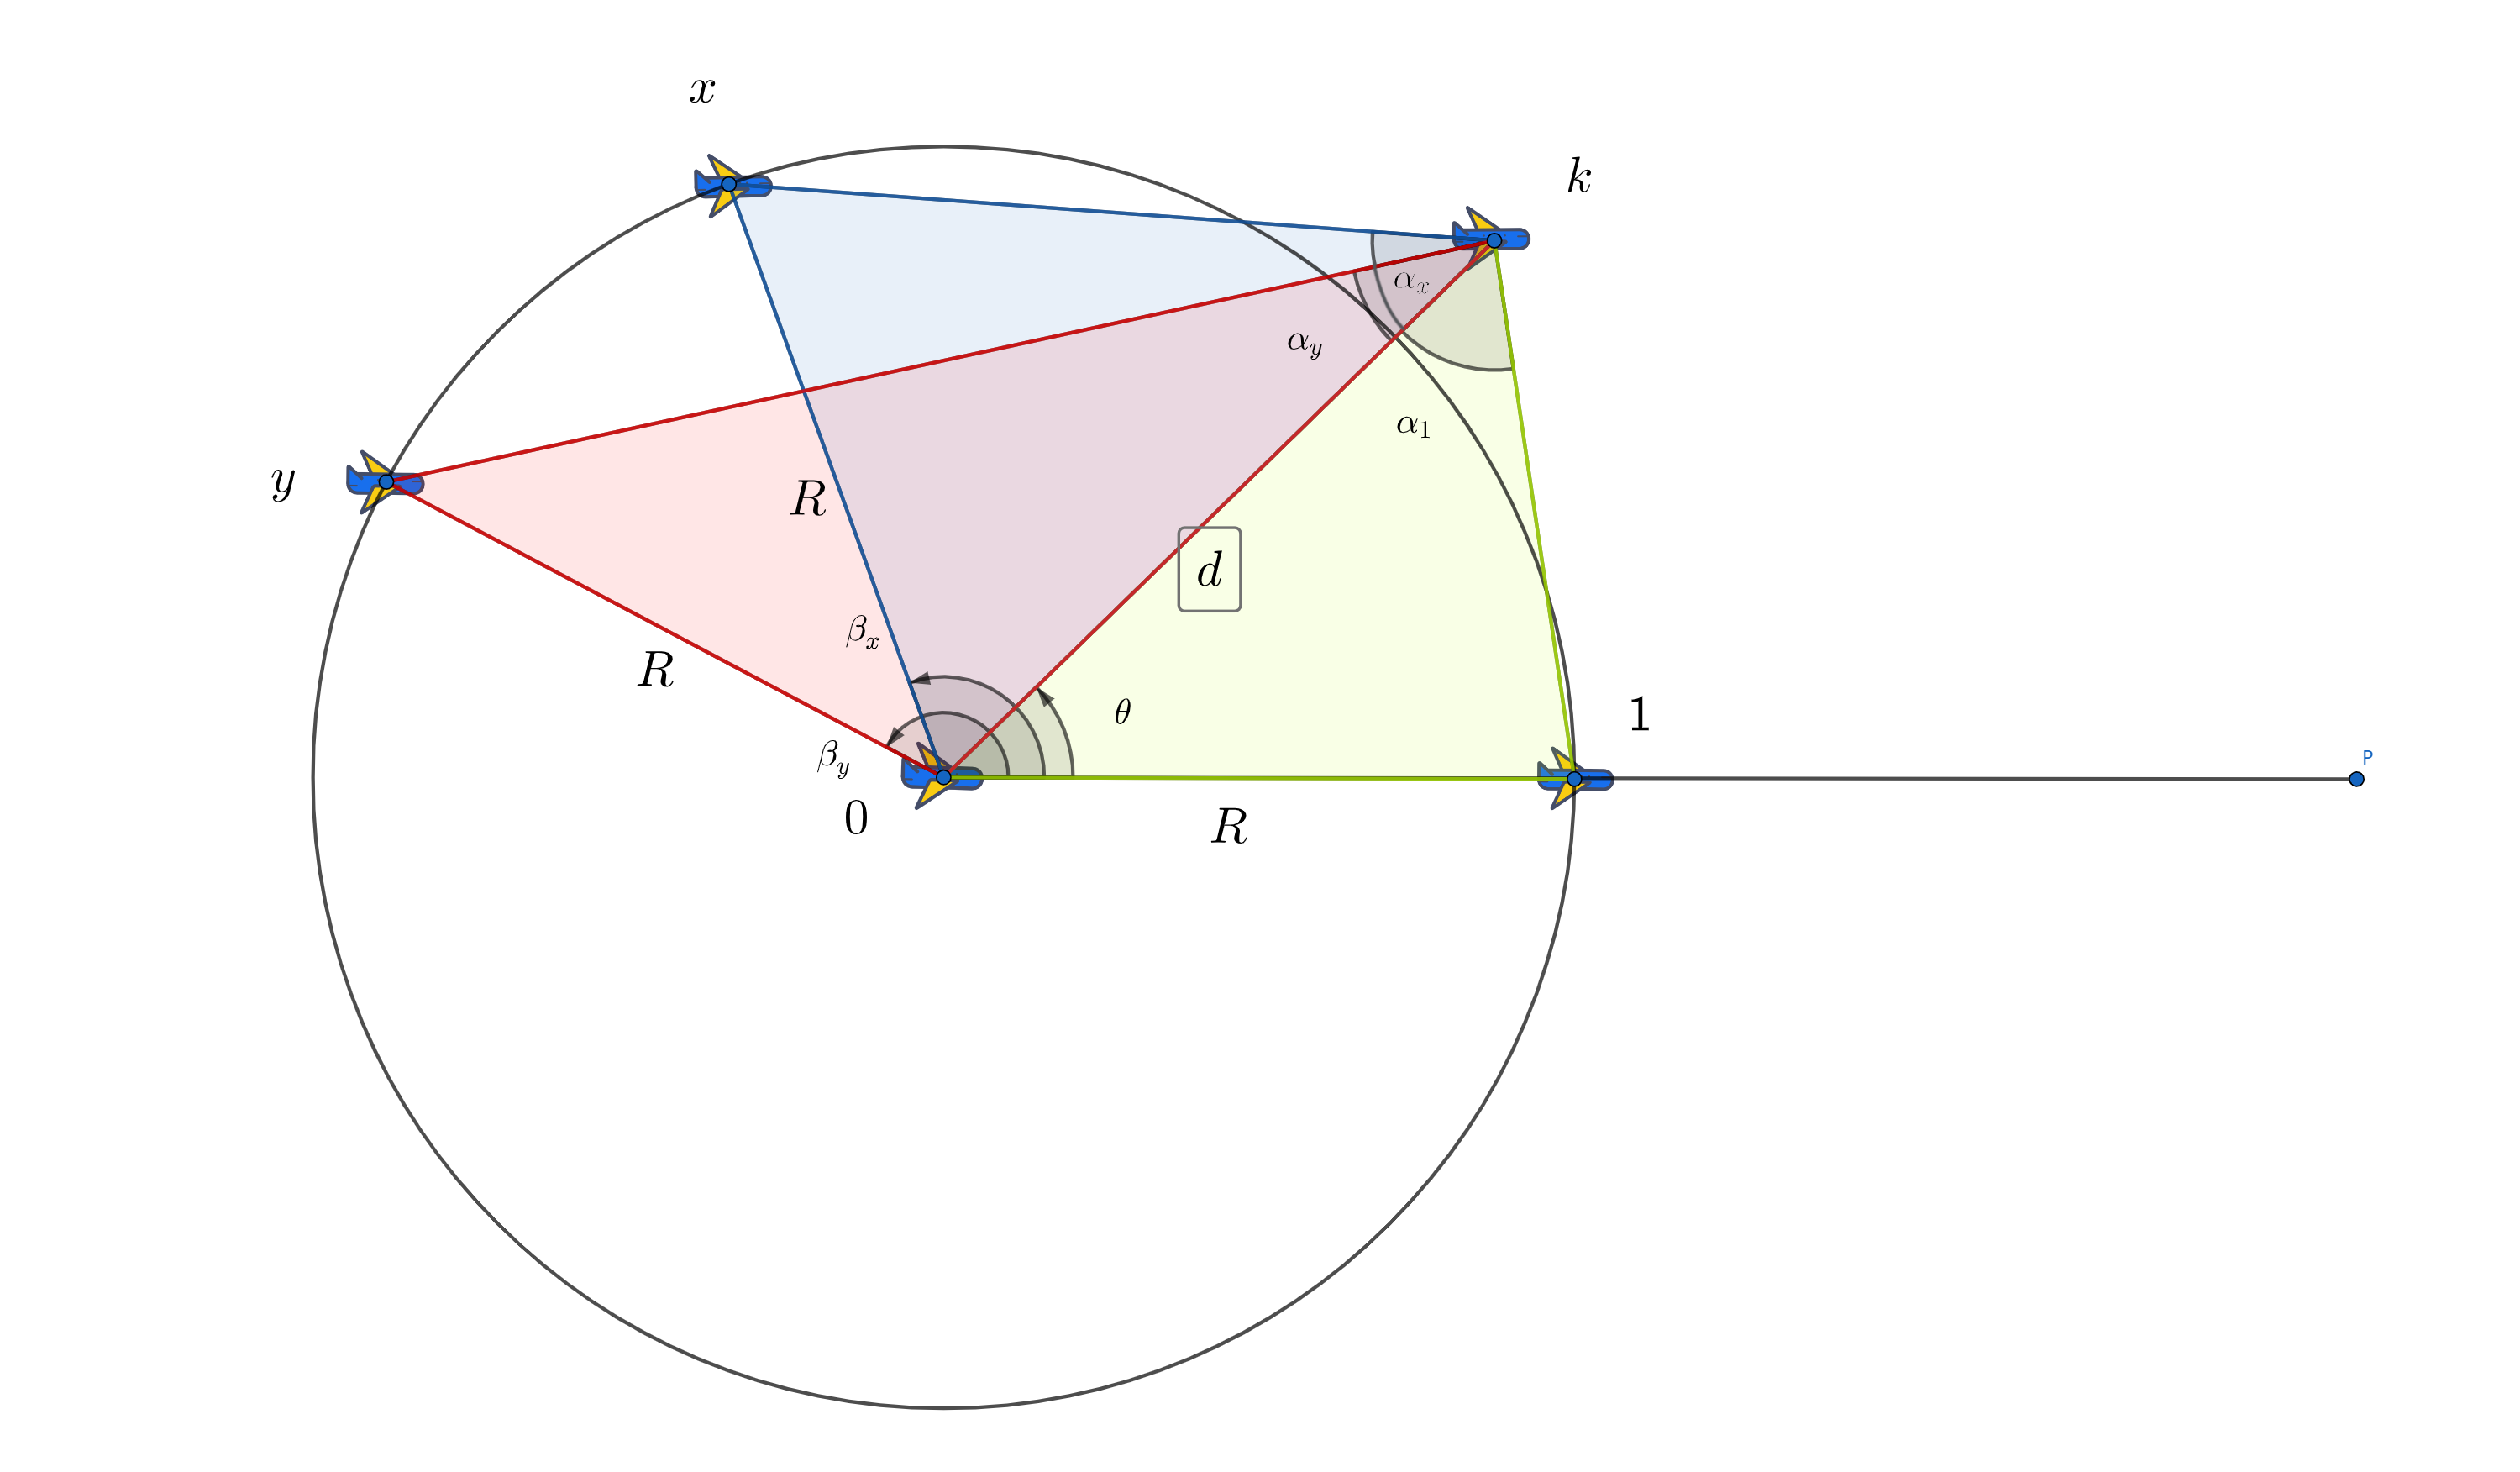
\includegraphics[width=1.0\textwidth]{figures/T2 fig3_.png}
    \caption{情形二添加两架无人机实现有效定位示意图}
    \label{fig:pos2}
\end{figure}


下面开始分析,对图中三个三角形使用正弦定理,得到的式子如下:
\begin{equation}
\left\{\begin{array}{lccr}
\frac{d}{\sin \left(\theta + \alpha_1\right)}=\frac{R}{\sin \alpha_1}  &  &&(a)\\
\frac{d}{\sin \left(\beta_x  - \theta + \alpha_x\right)}=\frac{R}{\sin \alpha_x} & &&(b)\\
\frac{d}{\sin \left(\beta_y  - \theta + \alpha_y\right)}=\frac{R}{\sin \alpha_y} & &&(c)
\end{array}\right.
\label{eq:abc}
\end{equation}

其中,$\beta_x= \frac{2}{9}\pi\cdot(x-1),\beta_y= \frac{2}{9}\pi\cdot(y-1)$。

以下考虑$\beta_y-\beta_x$和$\alpha_x-\alpha_y$的关联,注意到$k$的偏离不至于过大时,
$$\lvert 0.5\cdot(\beta_y-\beta_x)-(\alpha_x-\alpha_y) \rvert<\frac{1}{18}\pi$$

又$\beta_y-\beta_x$为$\frac{2}{9}\pi$的倍数,从而可以由$\alpha_x-\alpha_y$唯一确定$\beta_y-\beta_x$。\\

设$\beta_y-\beta_x=t$,代入方程\ref{eq:abc}求解。先联立\ref{eq:abc}$b$和\ref{eq:abc}$c$,类似5.1,可以得到$\beta_x-\theta$的唯一解,之后再联立\ref{eq:abc}$a$和\ref{eq:abc}$b$,可以得到$\theta$和$d$的唯一解,即实现了无人机$k$的有效定位。

对于其他情形,类似地可以用已知角的大小关系,确定$1,x,y$中的至少一组距离差。如果可以确定$x$或$y$和1的距离差,则可以用5.1的方法实现有效定位;如果可以确定$x$和$y$的距离差,则同样可以代入方程\ref{eq:abc}完成有效定位。

综上所述,这类情形中,还需要两架无人机发射信号,才能实现无人机的有效定位。

\subsection{第三个任务}
\subsubsection{算法分析}
设$x_k^{(t)}$为无人机$k$在时刻$t$所在的坐标。
设$F_k,k\in \{1,2,\dots, N\}$为半径100m圆周上均匀分布的N个点的坐标(本题中$N=9$),是第$k$号无人机需要尽可能接近的目标。特别地,$F_1$是无人机FY01的坐标,作为极坐标系极轴的基准点。
则定义:无人机调整的目标函数是每一架无人机和其目标的距离的总和(这里乘以$\frac{1}{2}$是为了求导便利)。

令
$$\textbf{x}^{(t)}=(x_1^{(t)},x_2^{(t)}, \dots, x_N^{(t)})$$
$$d_k(x_k^{(t)}) = \frac{1}{2} (x_k^{(t)}-F_k)^2$$

问题目标:
\begin{equation}
    \min_{x_1,x_2,\dots, x_N}  \sum_{k=1}^N d_k(x_k^{(t)})
\end{equation}

对$d_k$求导得:
$$\frac{\partial d_k}{\partial x_k^{(t)}}= x_k^{(t)} - F_k$$

所以
\begin{gather*}
    \nabla_{x_k^{(t)}} \sum_{k=1}^N d_k(x_k^{(t)}) 
    = \sum_{k=1}^N \nabla_{x_k^{(t)}}  d_k(x_k^{(t)}) 
    = (x_1^{(t)} - F_1, x_2^{(t)} - F_2, \dots, x_N^{(t)} - F_N)^\top
\end{gather*}

使用梯度下降法最小化目标函数,更新方程为:

\begin{equation}
    \textbf{x}^{(t+1)} \gets \textbf{x}^{(t)} - \eta \nabla_{x_k^{(t)}} \sum_{k=1}^N d_k(x_k^{(t)}) 
\end{equation}

化为分量形式:
\begin{equation}\label{gd_k}
    x_k^{(t+1)} \gets x_k^{(t)} - \eta \frac{\partial d_k}{\partial x_k^{(t)}} = (1-\eta) x_k^{(t)} + \eta F_k
\end{equation}

在\ref{1.1}中已经证明了,在发射信号的无人机$i$和无人机$j$编号已知且位置无偏差的情况下,能够准确定位接收信号的无人机$k$。但在第三小问中,发射信号的无人机$i,j$本身位置存在偏差,因此利用\ref{1.1}中模型所接收信号的无人机$k$的位置也和其真实坐标有偏差。

由于题目条件中初始时刻$(t=0)$时无人机位置仅有略微偏差,可以对接受信号的无人机测量结果的偏差作出简化假设:其测量结果坐标为真实坐标上叠加一个二维高斯噪声:
$$
\tilde{x_k}^{(t)} = x_k^{(t)} + Y,Y\sim \mathcal{N}(\textbf{0},{{\Sigma}})
$$,
其中$\tilde{x_k}^{(t)}$是无人机$k$坐标的测量值,$x_k^{(t)}$是真实值,$\Sigma$是协方差矩阵。
则更新方程变为:
\begin{equation}
    x_k^{(t+1)} \gets (1-\eta) (\tilde{x_k}^{(t)} - Y) + \eta F_k = (1-\eta) \tilde{x_k}^{(t)} + \eta F_k + \eta Y
\end{equation}
与\ref{gd_k}对比,将$x_k^{(t)}$换为有误差的$\tilde{x_k}^{(t)}$时,相当于在更新方程等号右侧多加上一个二维高斯噪声。这种梯度下降的更新方式在文献中称为“含噪声的梯度下降法(Noisy Gradient Descent)”。

研究表明,当梯度下降中含有期望为为0的高斯噪声,仍然能够保证变量收敛在局部最小值的一个小邻域内\cite{wu2020noisy}\cite{smith2020generalization};这一点和在机器学习算法中常见的随机梯度下降算法(Stochastic Gradient Descent, SGD)的收敛性的证明方法相类似,而SGD算法在实际问题中被证明有良好的收敛性,并且能够一定程度上克服普通的梯度下降算法陷入局部最优解的问题。鉴于题目中无人机的位置偏差不大,且目标函数是$N$元二次函数,是凸函数,拥有唯一极小值点,因此可以认为目标函数最终能收敛到全局最小值$0$。

\subsubsection{算法实现}\label{Algo1}
上述算法的实现可由以下伪代码描述:
\begin{algorithm}[H]
	\caption{基于带噪声梯度下降的无人机编队位置调整算法} 
	\begin{algorithmic}[1]
    \State 初始化$(x_1^{(0)},x_2^{(0)}, \dots, x_N^{(0)})$为$N$架无人机初始位置 \Comment{本题中取$N=9$}
    \State $q\gets 1$ \Comment{选定参考点}
    \State 选定坐标原点(0,0)和极轴参考点$x_q^{(0)}$
    \State $M\gets 1000$ \Comment{迭代次数}
    \State $\eta \gets 0.5$ \Comment{梯度下降学习率}
    \For{$t:0\rightarrow M$}
        \State 随机选取$i, j, k$ 满足$i < j$且$i \ne k, j \ne k, k \ne q$
        \State 无人机$i,j$发射,无人机$k$获取角度观测值$\alpha_1,\alpha_2$和发射机角度$\beta_1,\beta_2$
        \State 根据\ref{1.1}中的四种情况图\ref{fig:classification},由\ref{1.1}求得无人机$k$坐标观测值$\tilde{x_k}^{(t)}$
        \State  
                    $$x_p^{(t+1)} \gets \begin{cases}
                        (1-\eta) \tilde{x_p}^{(t)} + \eta F_p & p=k \\
                        x_p^{(t+1)} & p\ne k
                    \end{cases}, p\in \{1,2,\dots, N\}
                    $$ \Comment{使用梯度下降法更新无人机$k$的位置,其余无人机位置不变}
                
    \EndFor
    \State $(x_1^{(M-1)},x_2^{(M-1)}, \dots, x_N^{(M-1)})$为无人机最终位置
	\end{algorithmic} 
	
\end{algorithm}
\subsubsection{实验效果}
按照题中数据运行\ref{Algo1}中算法,无人机的初始位置、调整轨迹和最终位置如下图\cite{辛沙欧2021基于纯方位的多无人机协同目标跟踪算法}:
\begin{figure}[H]
    \centering
    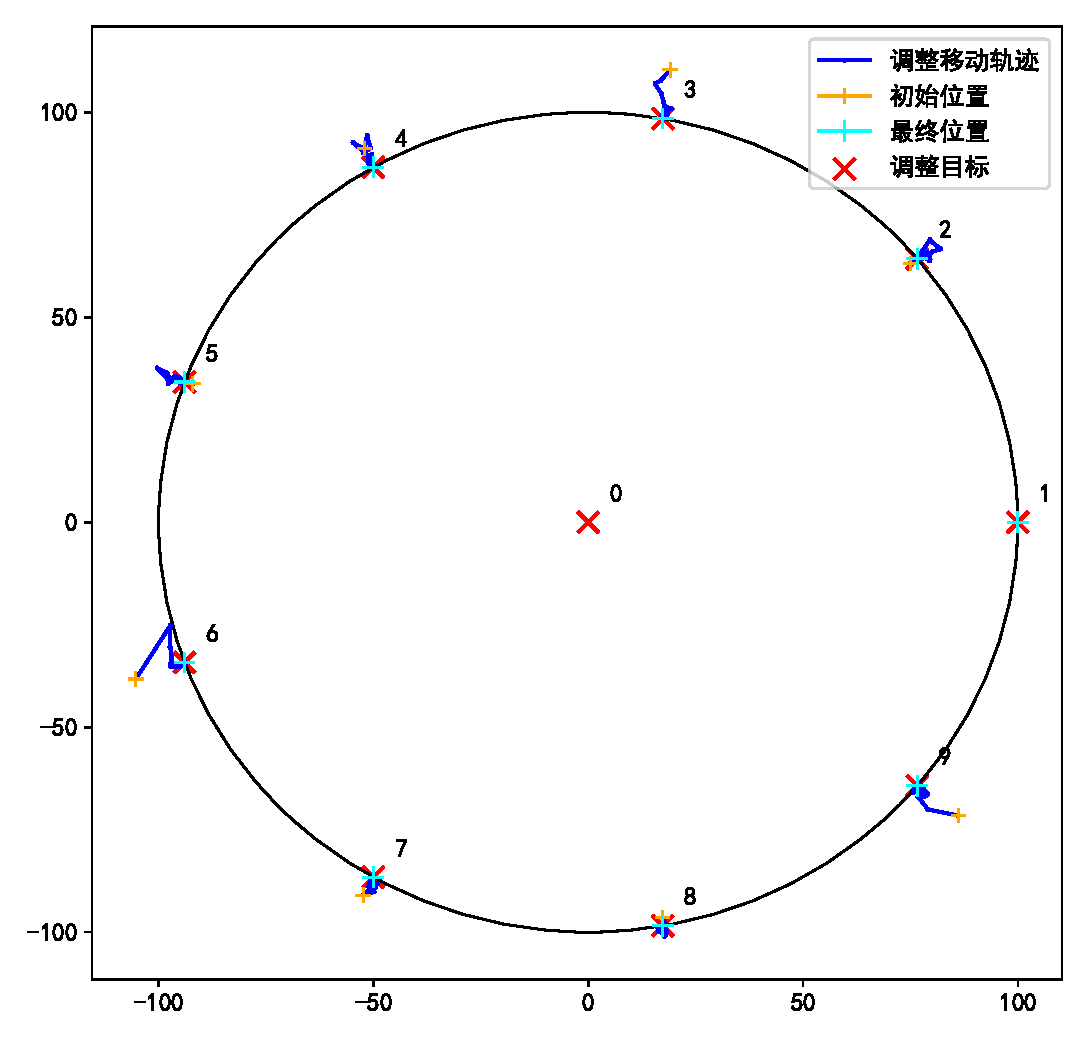
\includegraphics[width=0.7\linewidth]{figures/Circle9_0.pdf}
    \caption{每架无人机调整为均匀分布在半径$R=100m$圆周上之过程}
    \label{fig:Circle9_0}
\end{figure}
\begin{figure}[H]
    \centering
    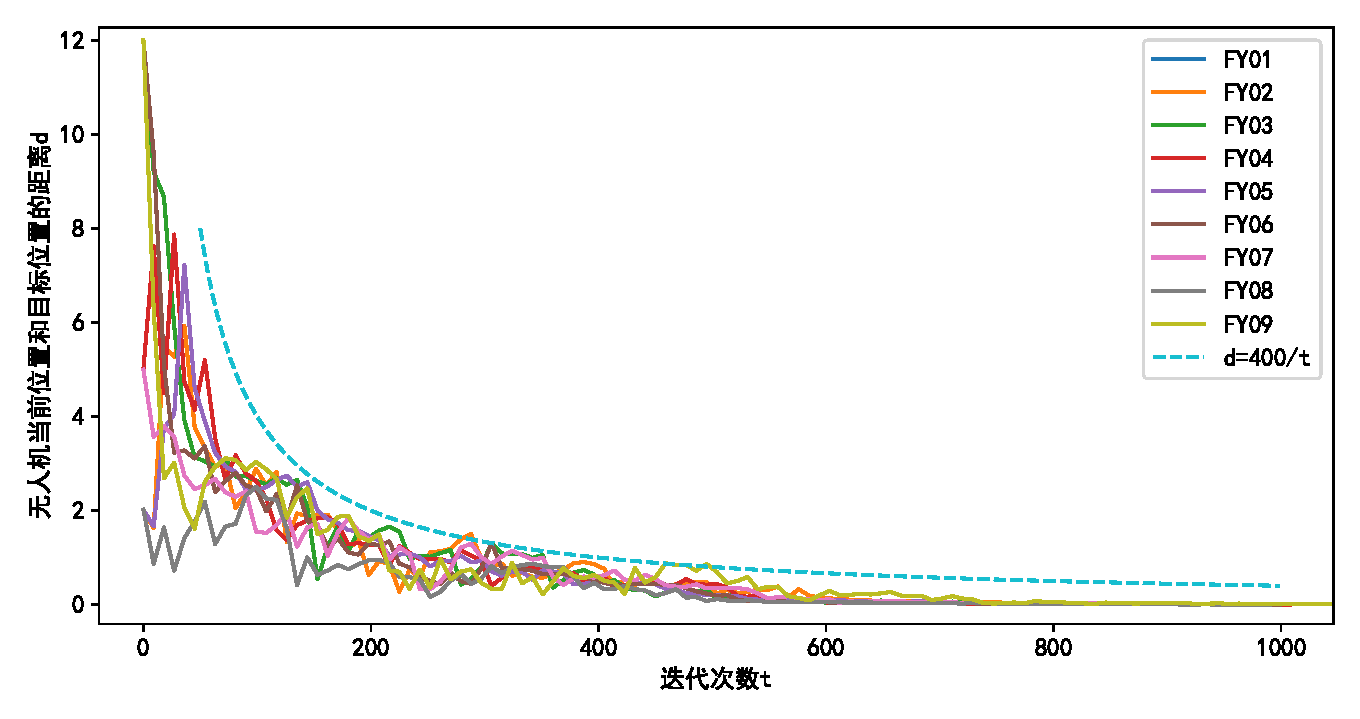
\includegraphics[width=0.9\linewidth]{figures/c9_convergence.pdf}
    \caption{九架无人机与其目标之间距离变化趋势}
    \label{fig:Circle9_Convergence}
\end{figure}

\begin{figure}[H]
    \centering
    \begin{subfigure}{0.32\linewidth}
        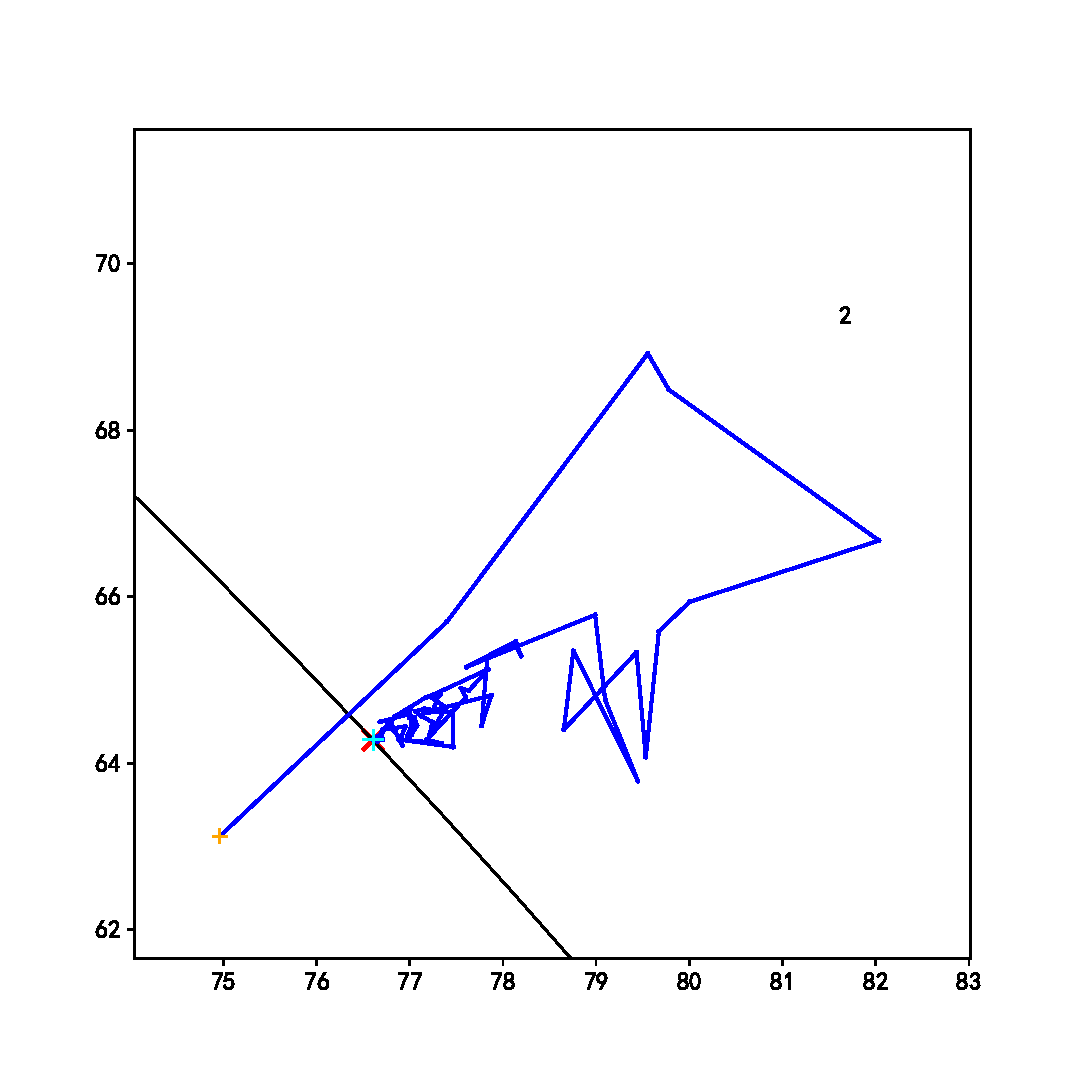
\includegraphics[width=1.1\linewidth]{figures/c9_2.pdf}
    \end{subfigure}
    \begin{subfigure}{0.32\linewidth}
        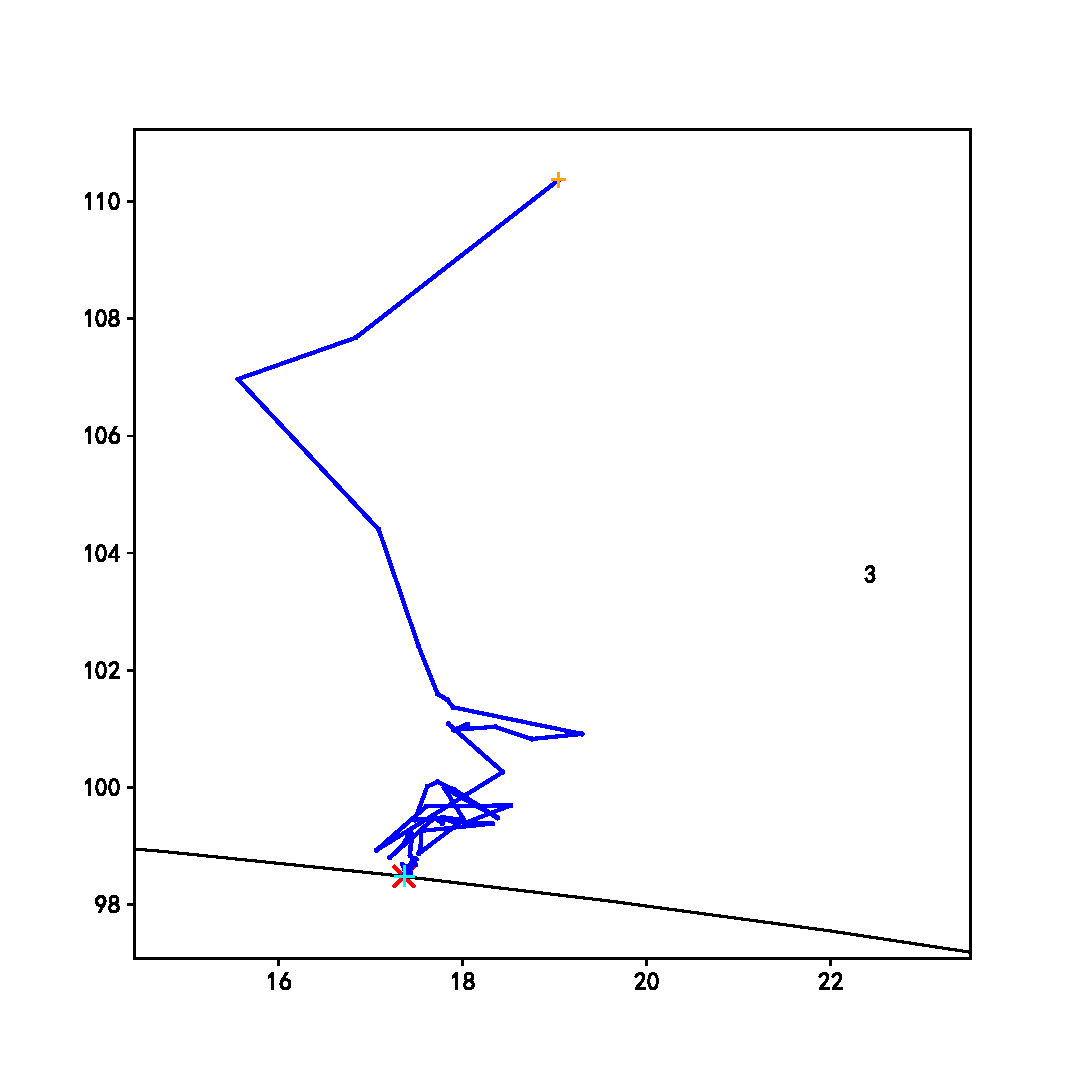
\includegraphics[width=1.1\linewidth]{figures/c9_3.pdf}
    \end{subfigure}
    \begin{subfigure}{0.32\linewidth}
        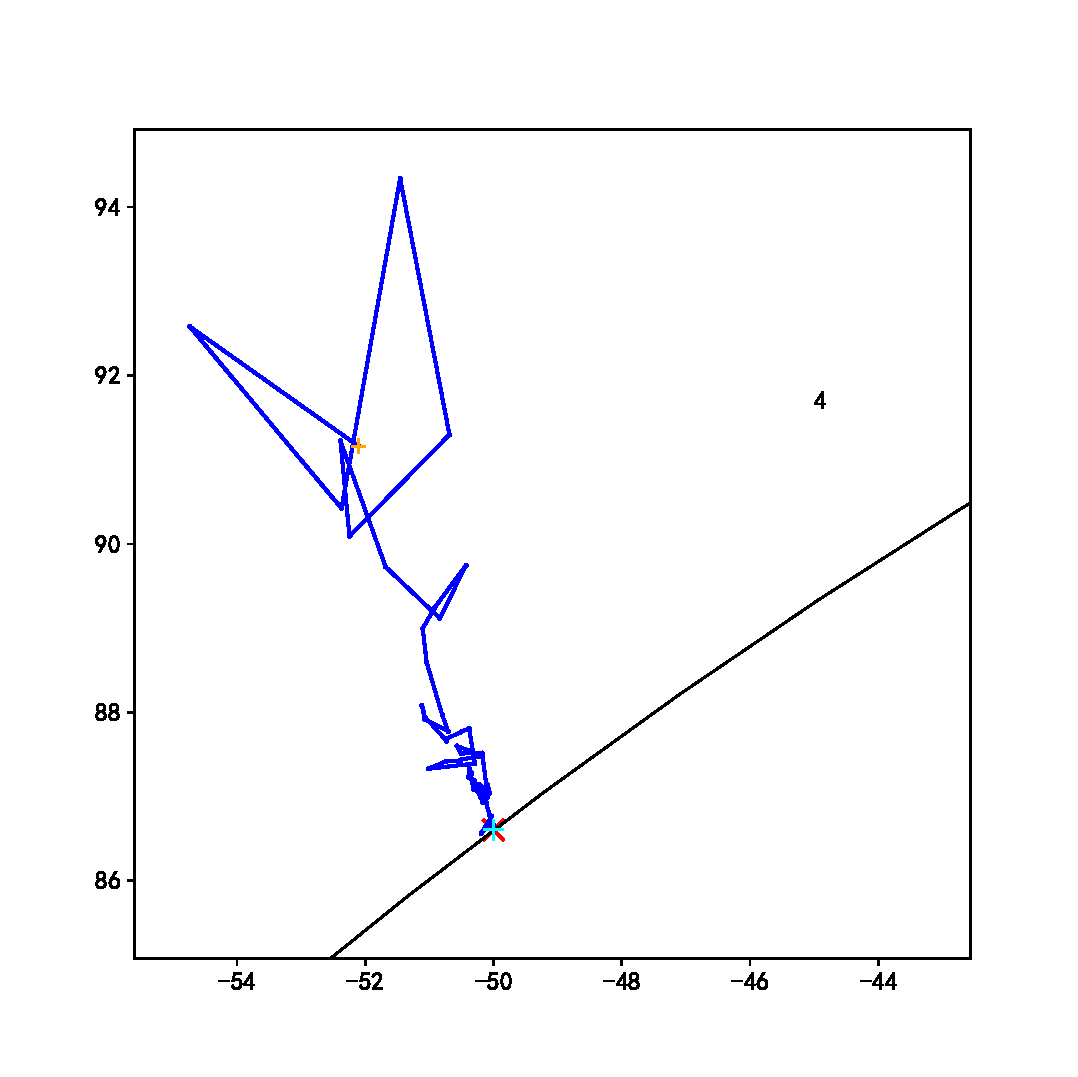
\includegraphics[width=1.1\linewidth]{figures/c9_4.pdf}
    \end{subfigure}
    \begin{subfigure}{0.32\linewidth}
        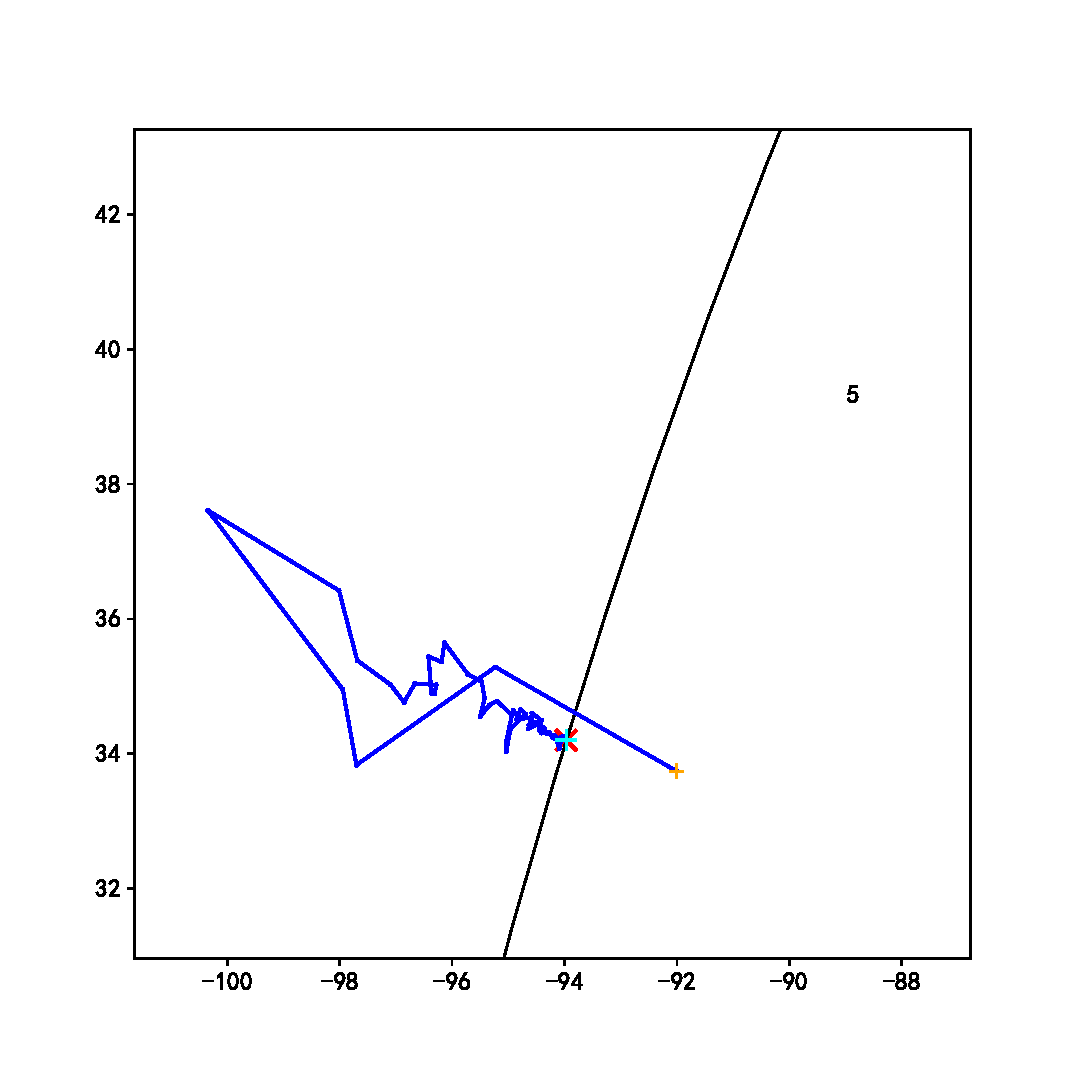
\includegraphics[width=1.1\linewidth]{figures/c9_5.pdf}
    \end{subfigure}
    \begin{subfigure}{0.32\linewidth}
        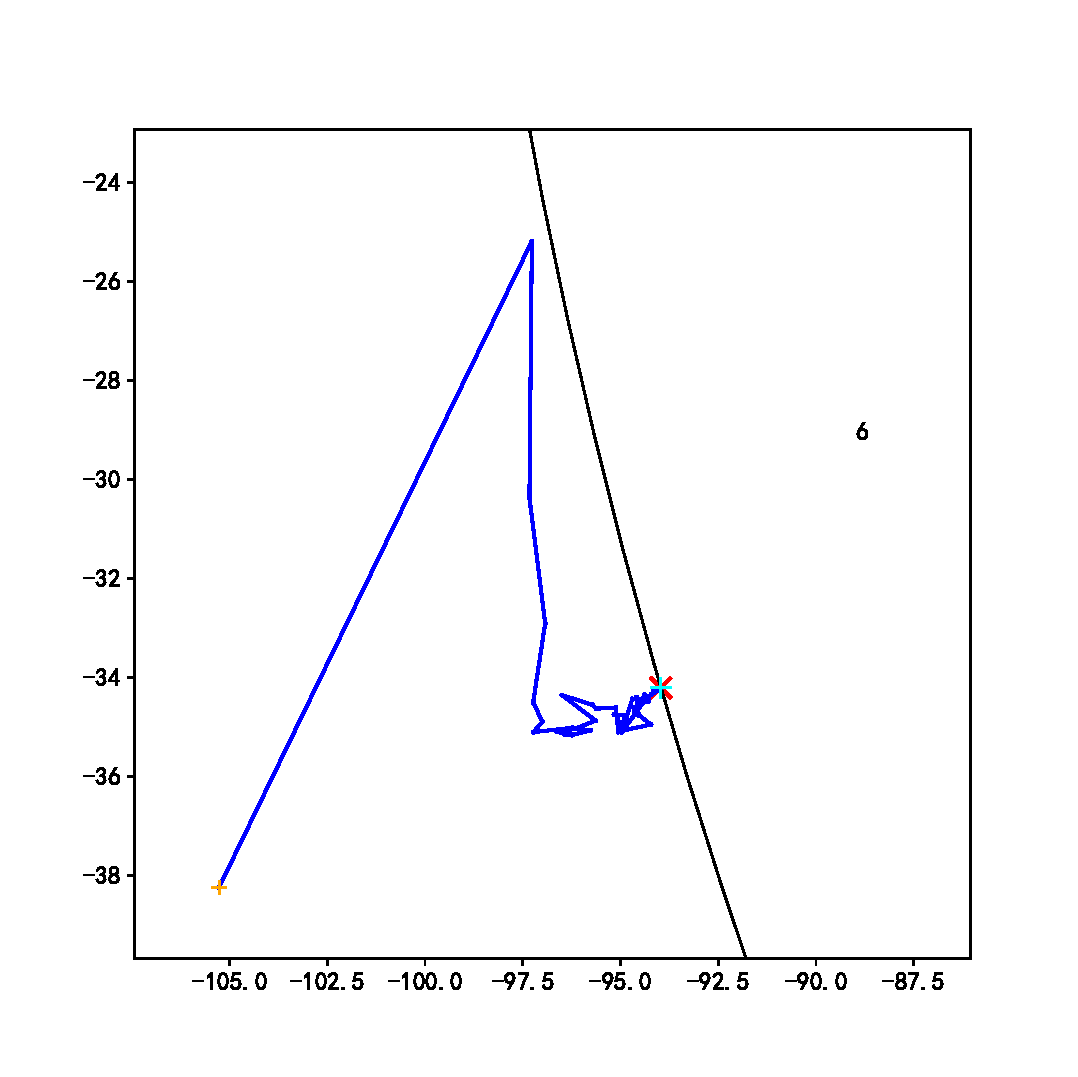
\includegraphics[width=1.1\linewidth]{figures/c9_6.pdf}
    \end{subfigure}
    \begin{subfigure}{0.32\linewidth}
        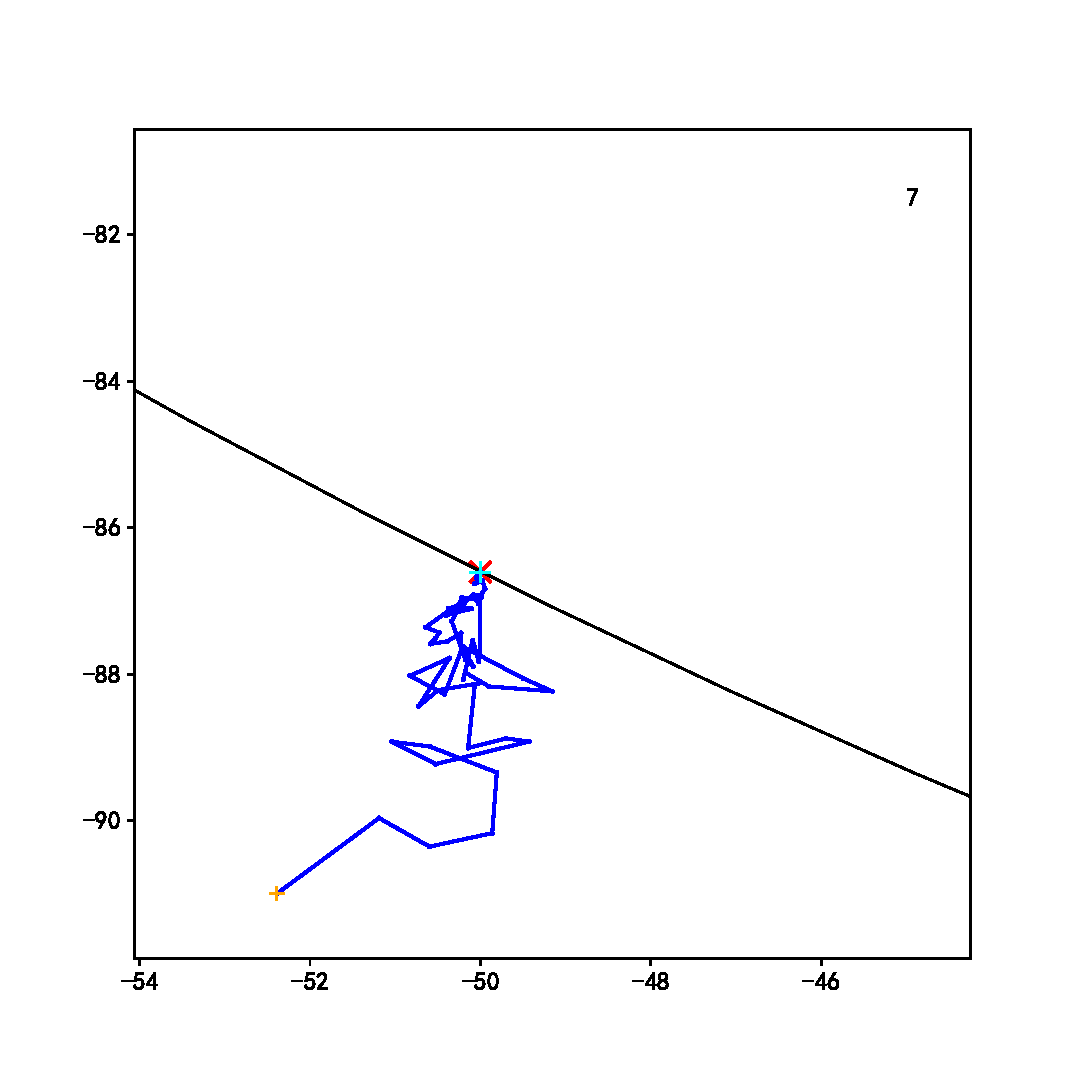
\includegraphics[width=1.1\linewidth]{figures/c9_7.pdf}
    \end{subfigure}
    \begin{subfigure}{0.32\linewidth}
        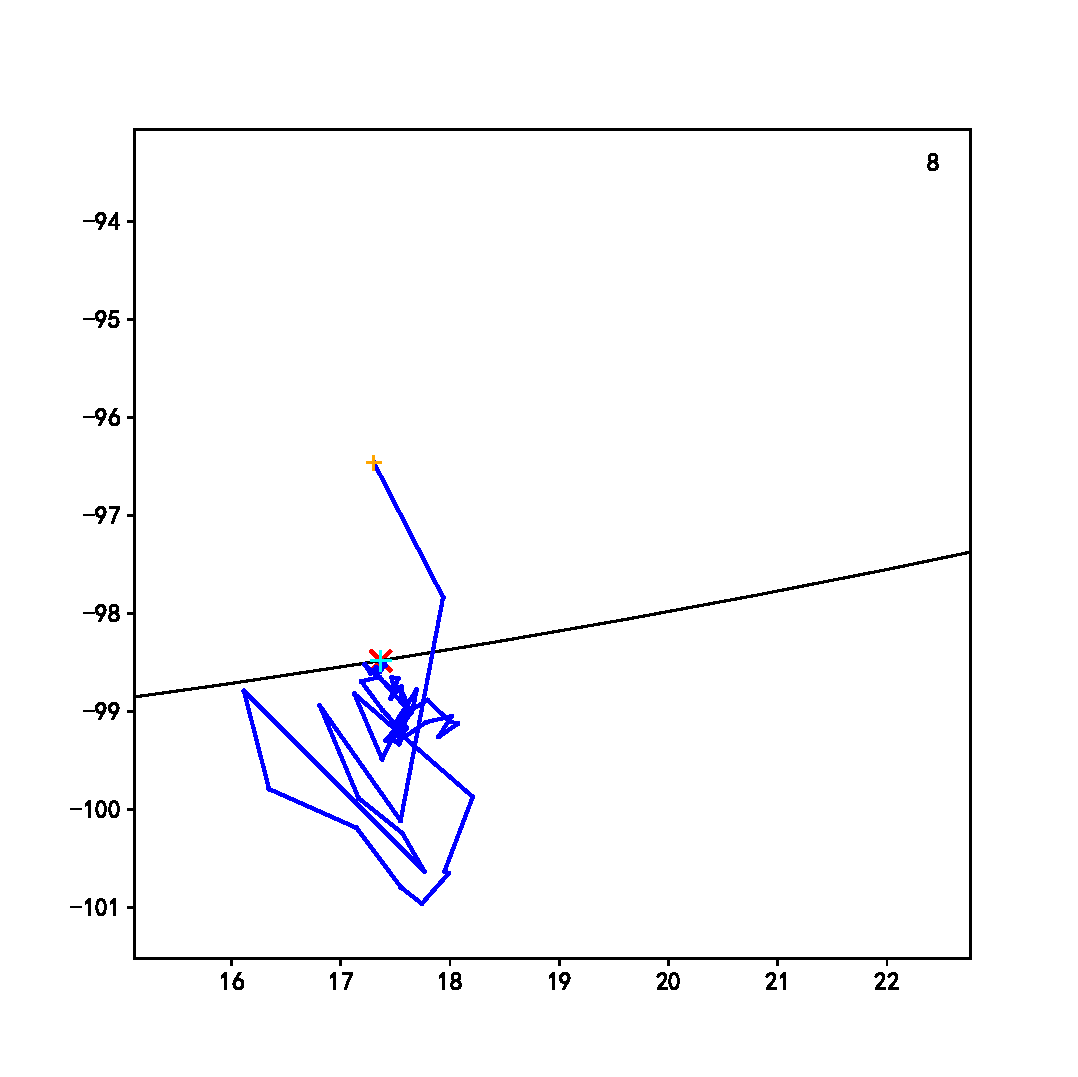
\includegraphics[width=1.1\linewidth]{figures/c9_8.pdf}
    \end{subfigure}
    \begin{subfigure}{0.32\linewidth}
        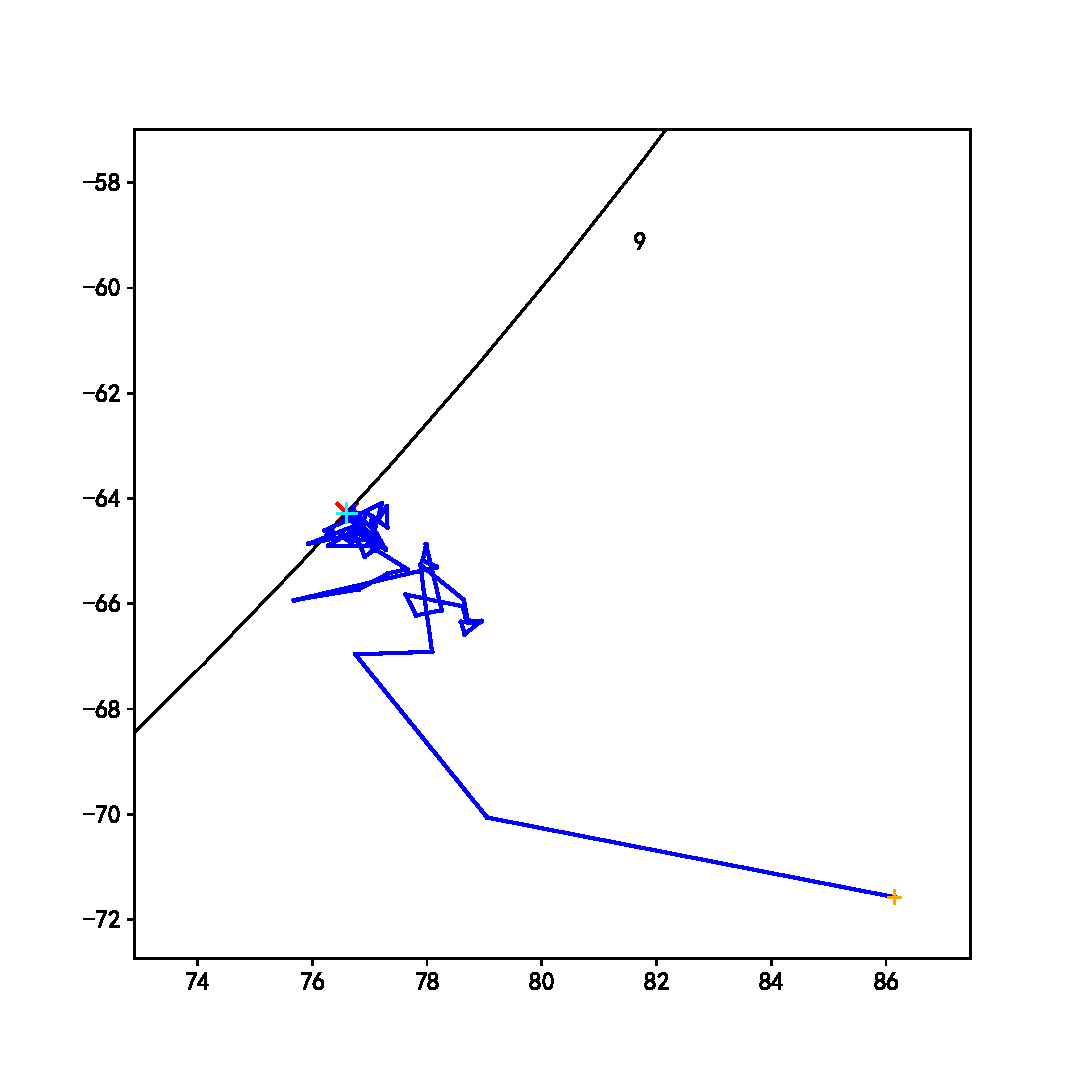
\includegraphics[width=1.1\linewidth]{figures/c9_9.pdf}
    \end{subfigure}
    \caption{调整过程细节放大图(图例解释同\ref{fig:Circle9_0})}
    \label{fig:C9_detail}
\end{figure}

从上图中可以看出,在无人机初始位置偏差如题设中数据时,算法能够较快地收敛,且所有无人机最终均匀分布于圆周上,和目标位置之间的距离趋近于0。因此可以认为该算法能够成功将无人机调整至理想位置。




\section{问题二的建模和分析}
\subsection{问题分析和求解}
本问题为考虑锥形编队队形无人机纯方位定位的位置调整问题。由于无人机两两之间距离均相等,如$R=50m$, 因此编队实际上可以拆分为等边三角形或正六边形。因此\ref{Algo1}中的算法仍然有效,我们只需要通过规划无人机的调整顺序,就可以实现将本问题化归为圆周上无人机均匀分布的问题,用同样的算法即可解决。

如下图所示,可以先调整以FY05为圆心、FY02为极轴参考点的极坐标系中和FY05相邻的六架无人机,使其均匀分布在圆周上。由\ref{Algo1}的结论,这六架无人机在调整后位置能够收敛到理想位置;这样的调整称为“七机圆形调整”。接着以FY08为圆心进行“七机圆形调整”:由于FY08,FY06已经在之前的调整中收敛到理想位置,则与FY008相邻的六架无人机在调整后也能够收敛到理想位置。同理,以FY09为圆心进行“七机圆形调整”。最终,除FY01, FY11, FY15外的无人机均收敛到理想位置,则这三架无人机也很能调整到理想位置,例如以FY03为圆心,FY02, FY05发射信号调整FY01的位置,其他同理。
\begin{figure}[H]
    \centering
    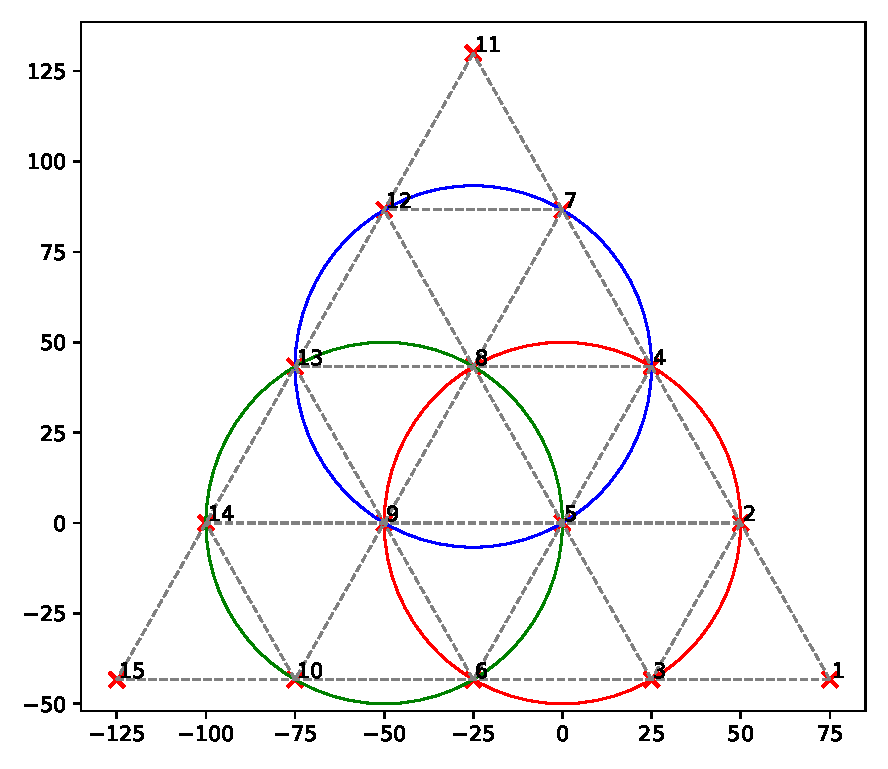
\includegraphics[width=0.7\linewidth]{figures/T2_0.pdf}
    \caption{通过三次圆形六等分调整使得锥形编队整体收敛于理想位置(红-蓝-绿顺序)}
    \label{fig:tri_0}
\end{figure}

\subsection{问题实验}

这里由于初始无人机偏移量较小,因此仅展示移动轨迹的细节图:\footnote{由于无人机的数目过多,此图仅选取部分展示。}
\begin{figure}[H]
    \centering
    \begin{subfigure}{0.45\linewidth}
        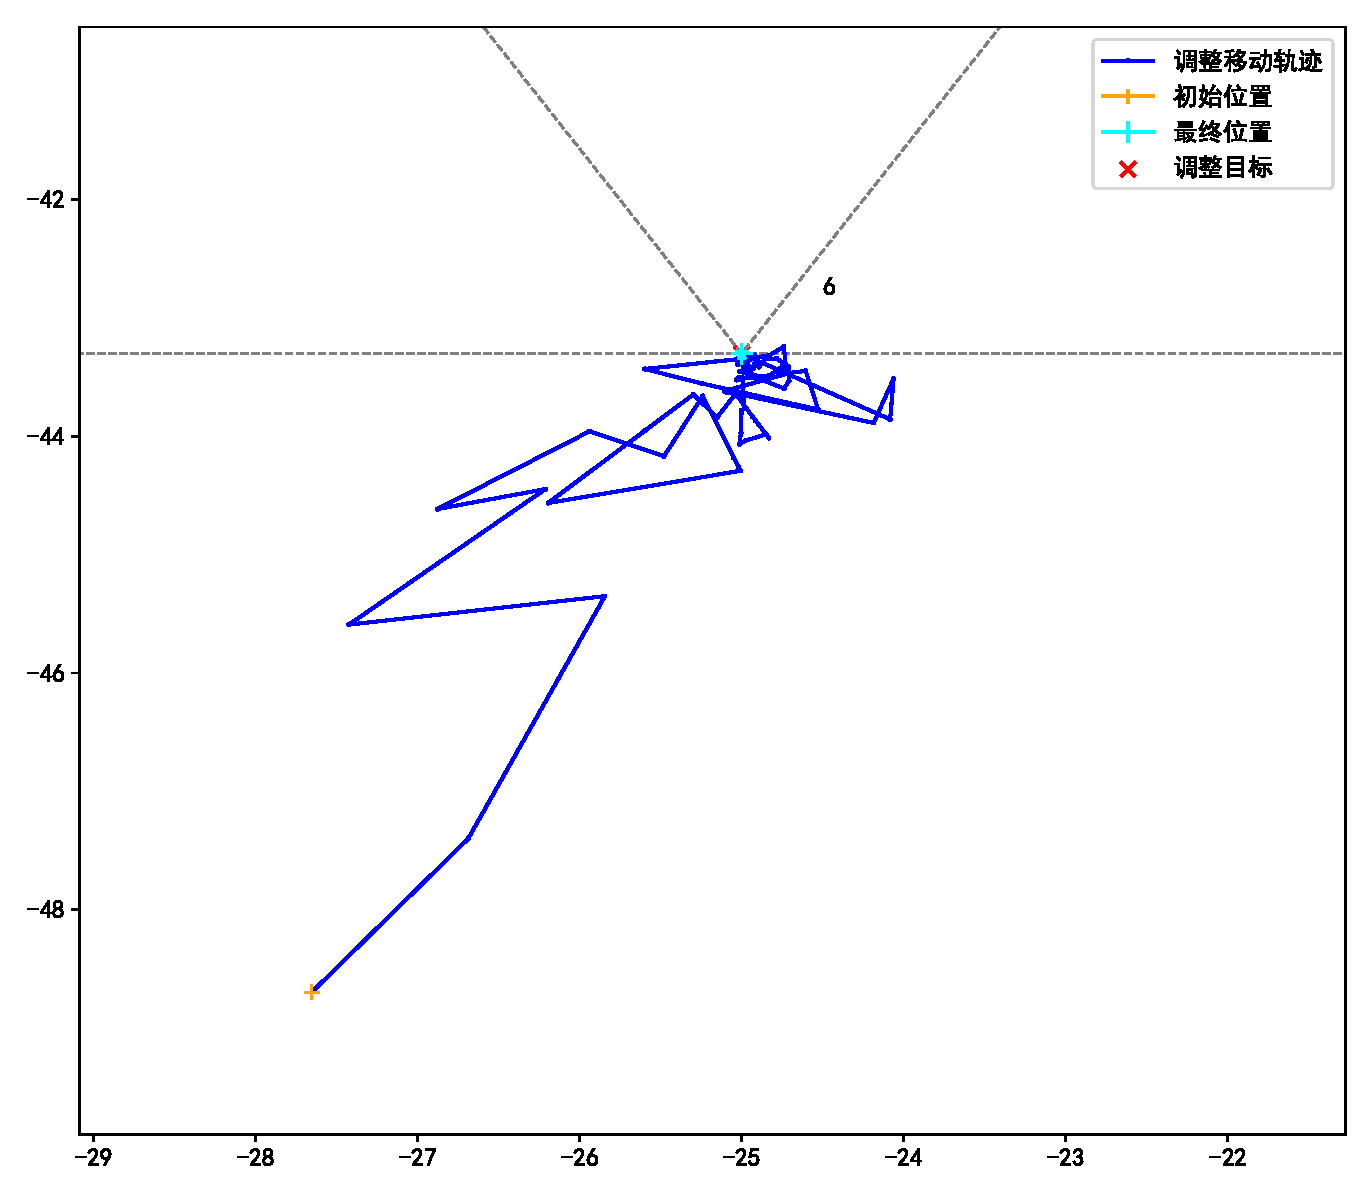
\includegraphics[width=1.0\linewidth]{figures/t_6.pdf}
    \end{subfigure}
    \begin{subfigure}{0.45\linewidth}
        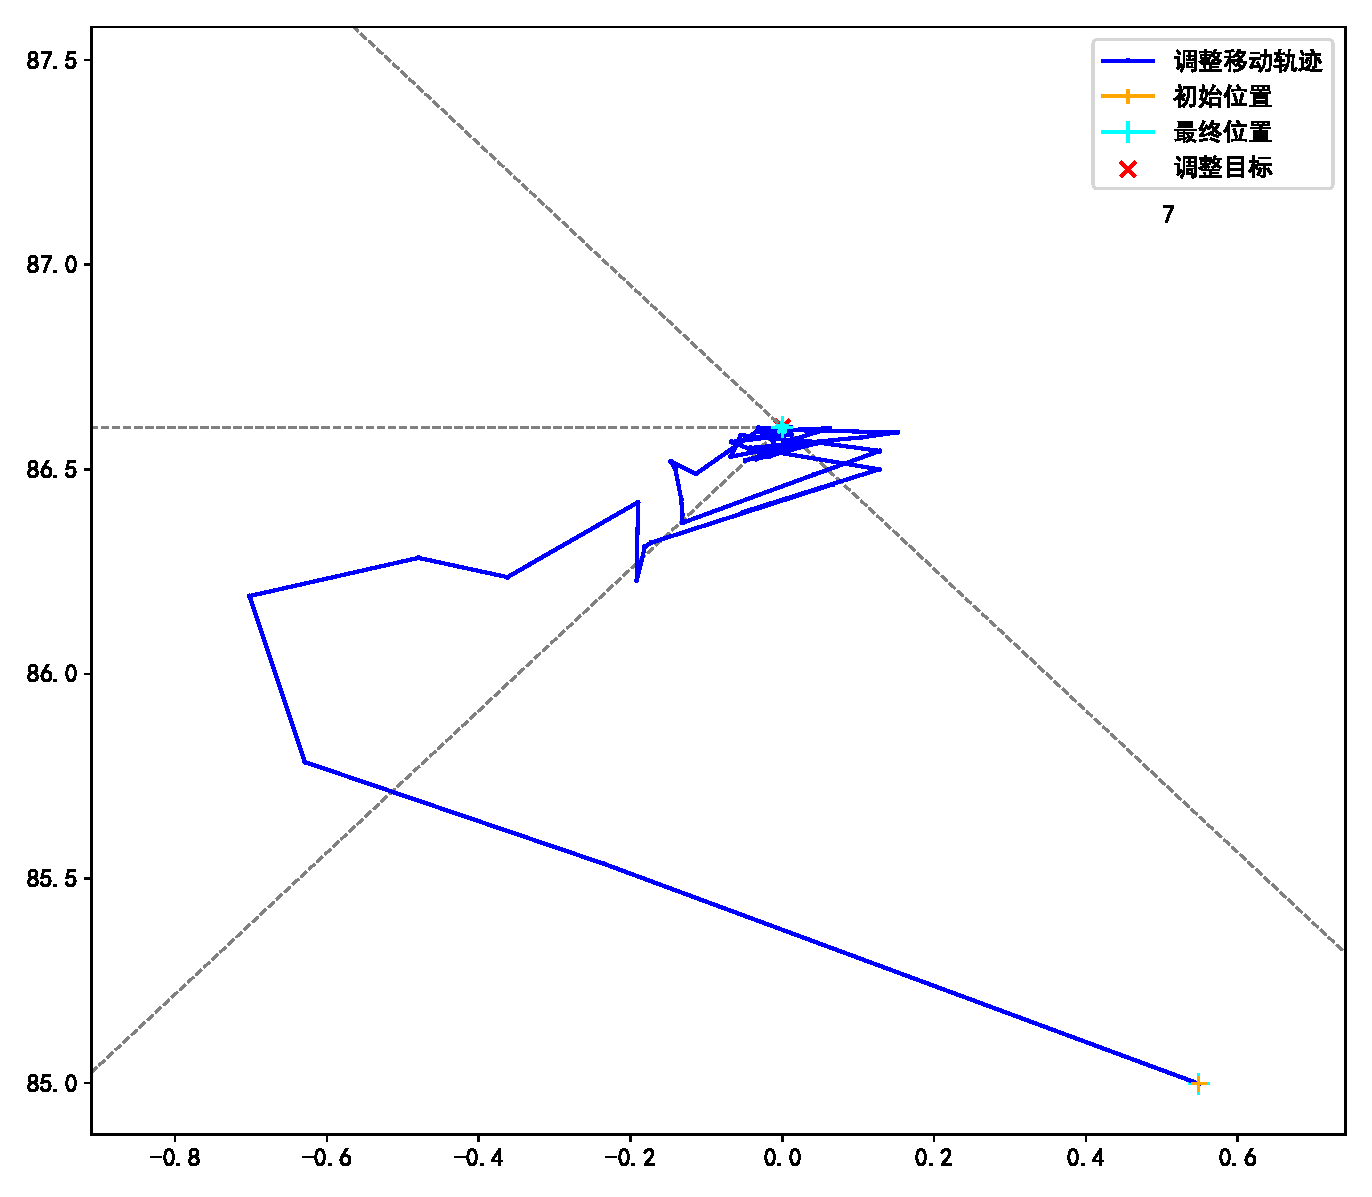
\includegraphics[width=1.0\linewidth]{figures/t_7.pdf}
    \end{subfigure}
    \begin{subfigure}{0.45\linewidth}
        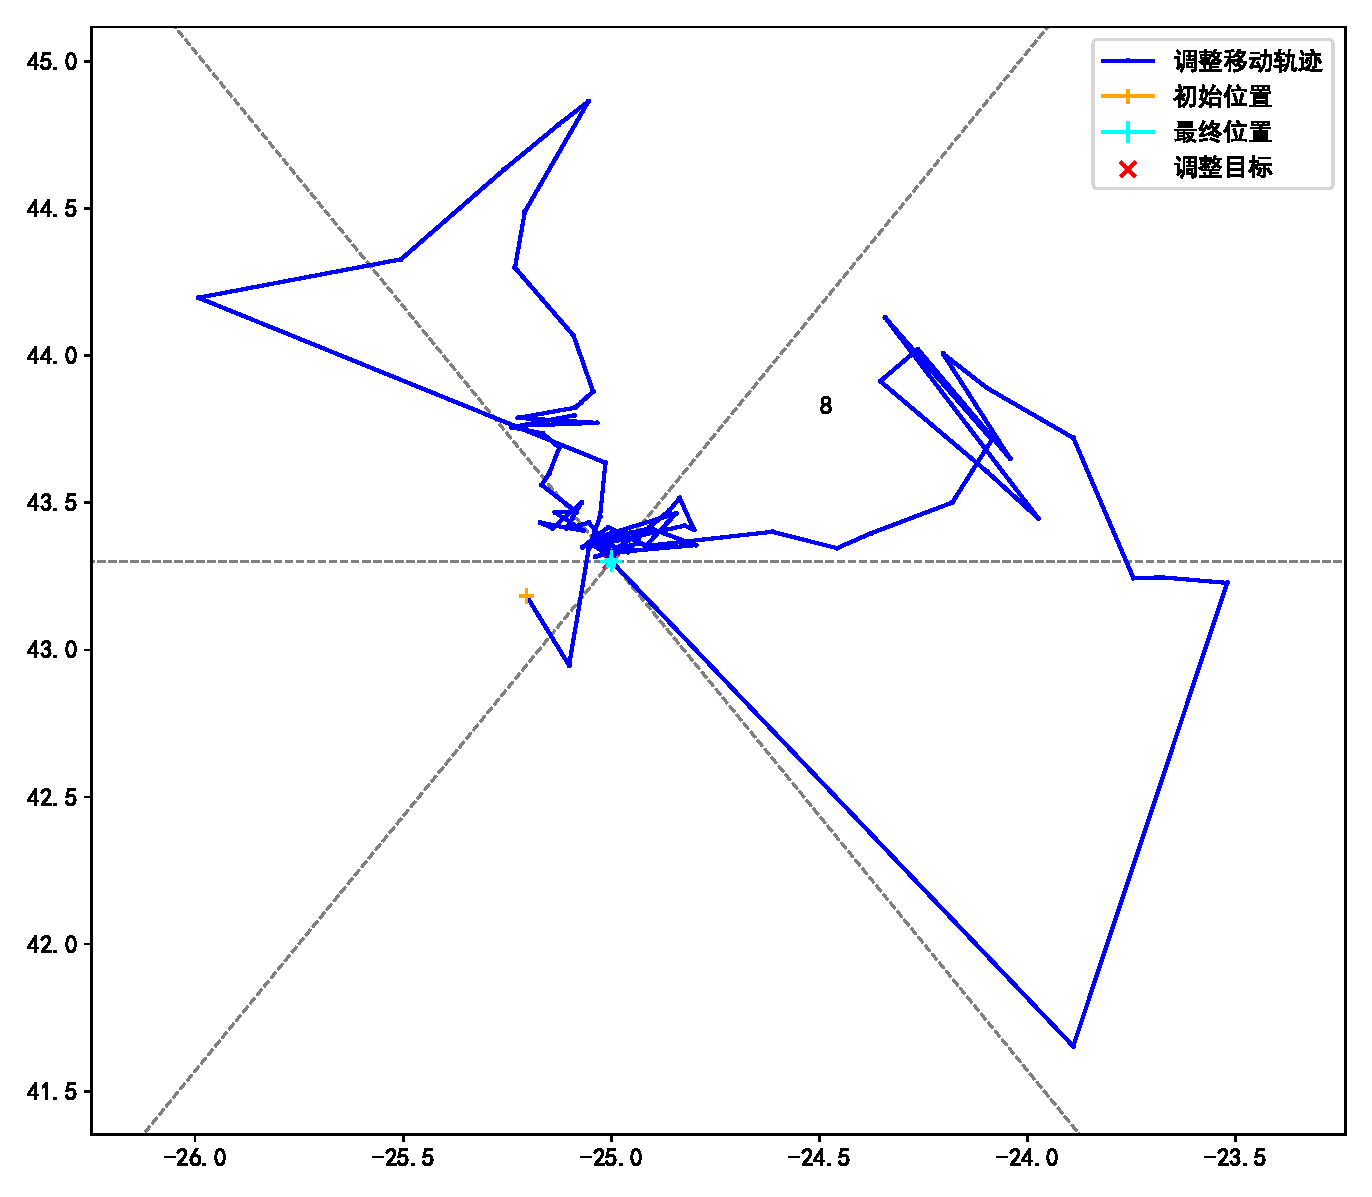
\includegraphics[width=1.0\linewidth]{figures/t_8.pdf}
    \end{subfigure}
    \begin{subfigure}{0.45\linewidth}
        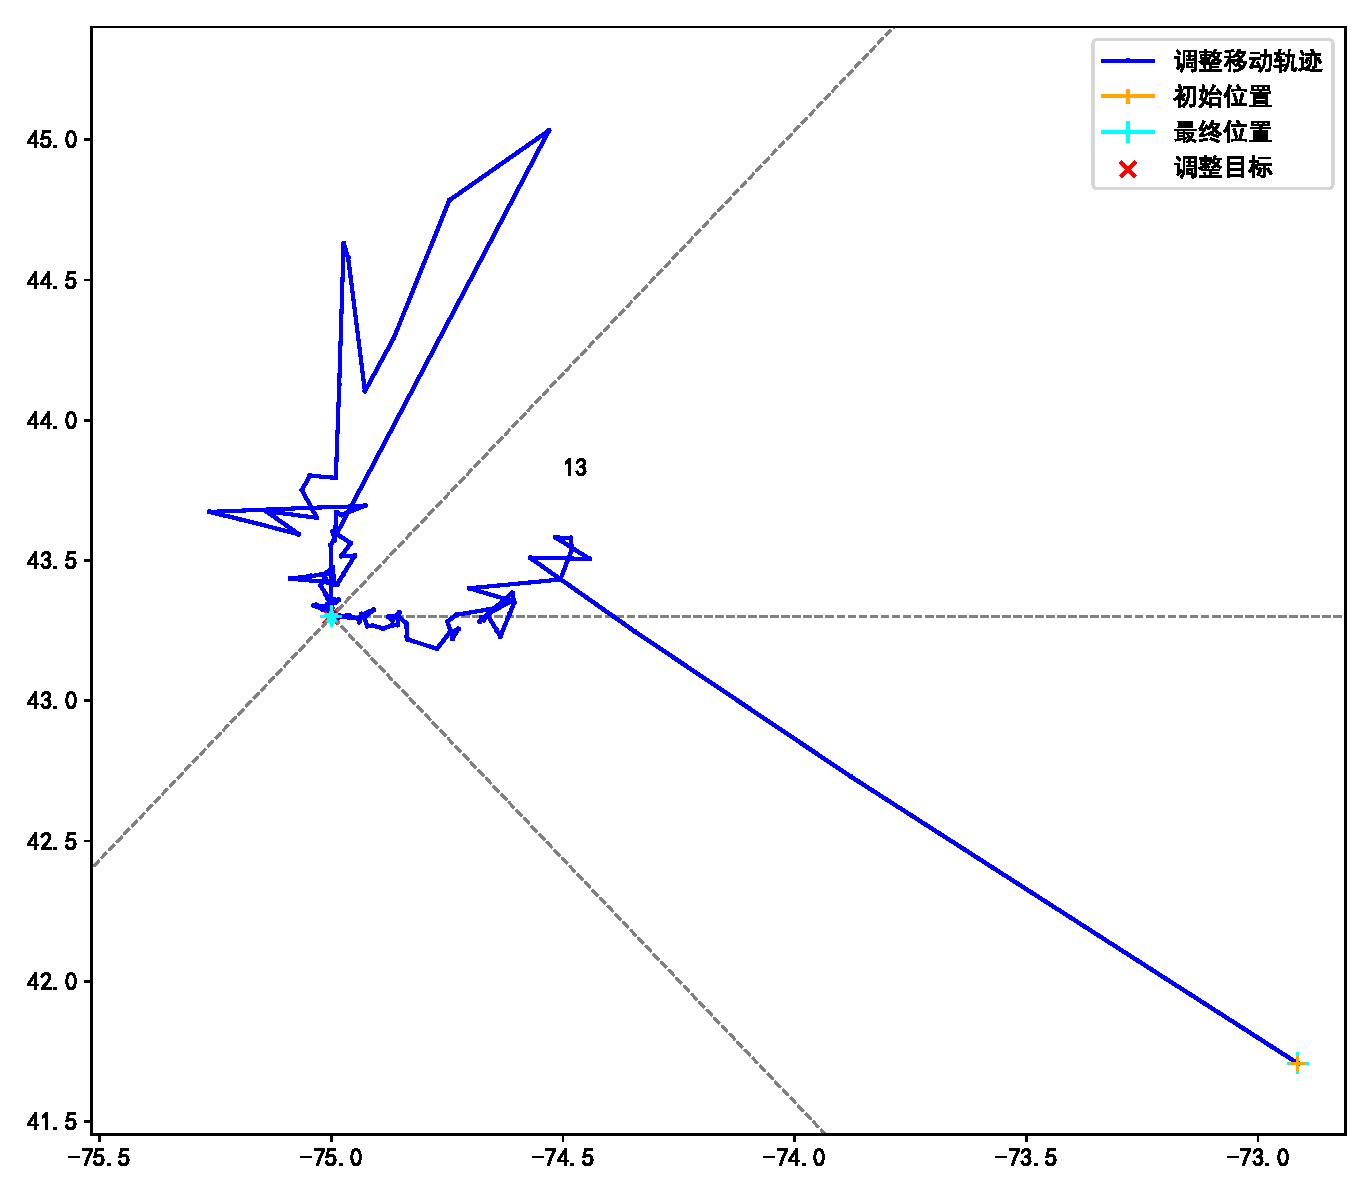
\includegraphics[width=1.0\linewidth]{figures/t_13.pdf}
    \end{subfigure}
    \caption{调整过程细节放大图}
    \label{fig:my_label}
\end{figure}

\begin{figure}[H]
    \centering
    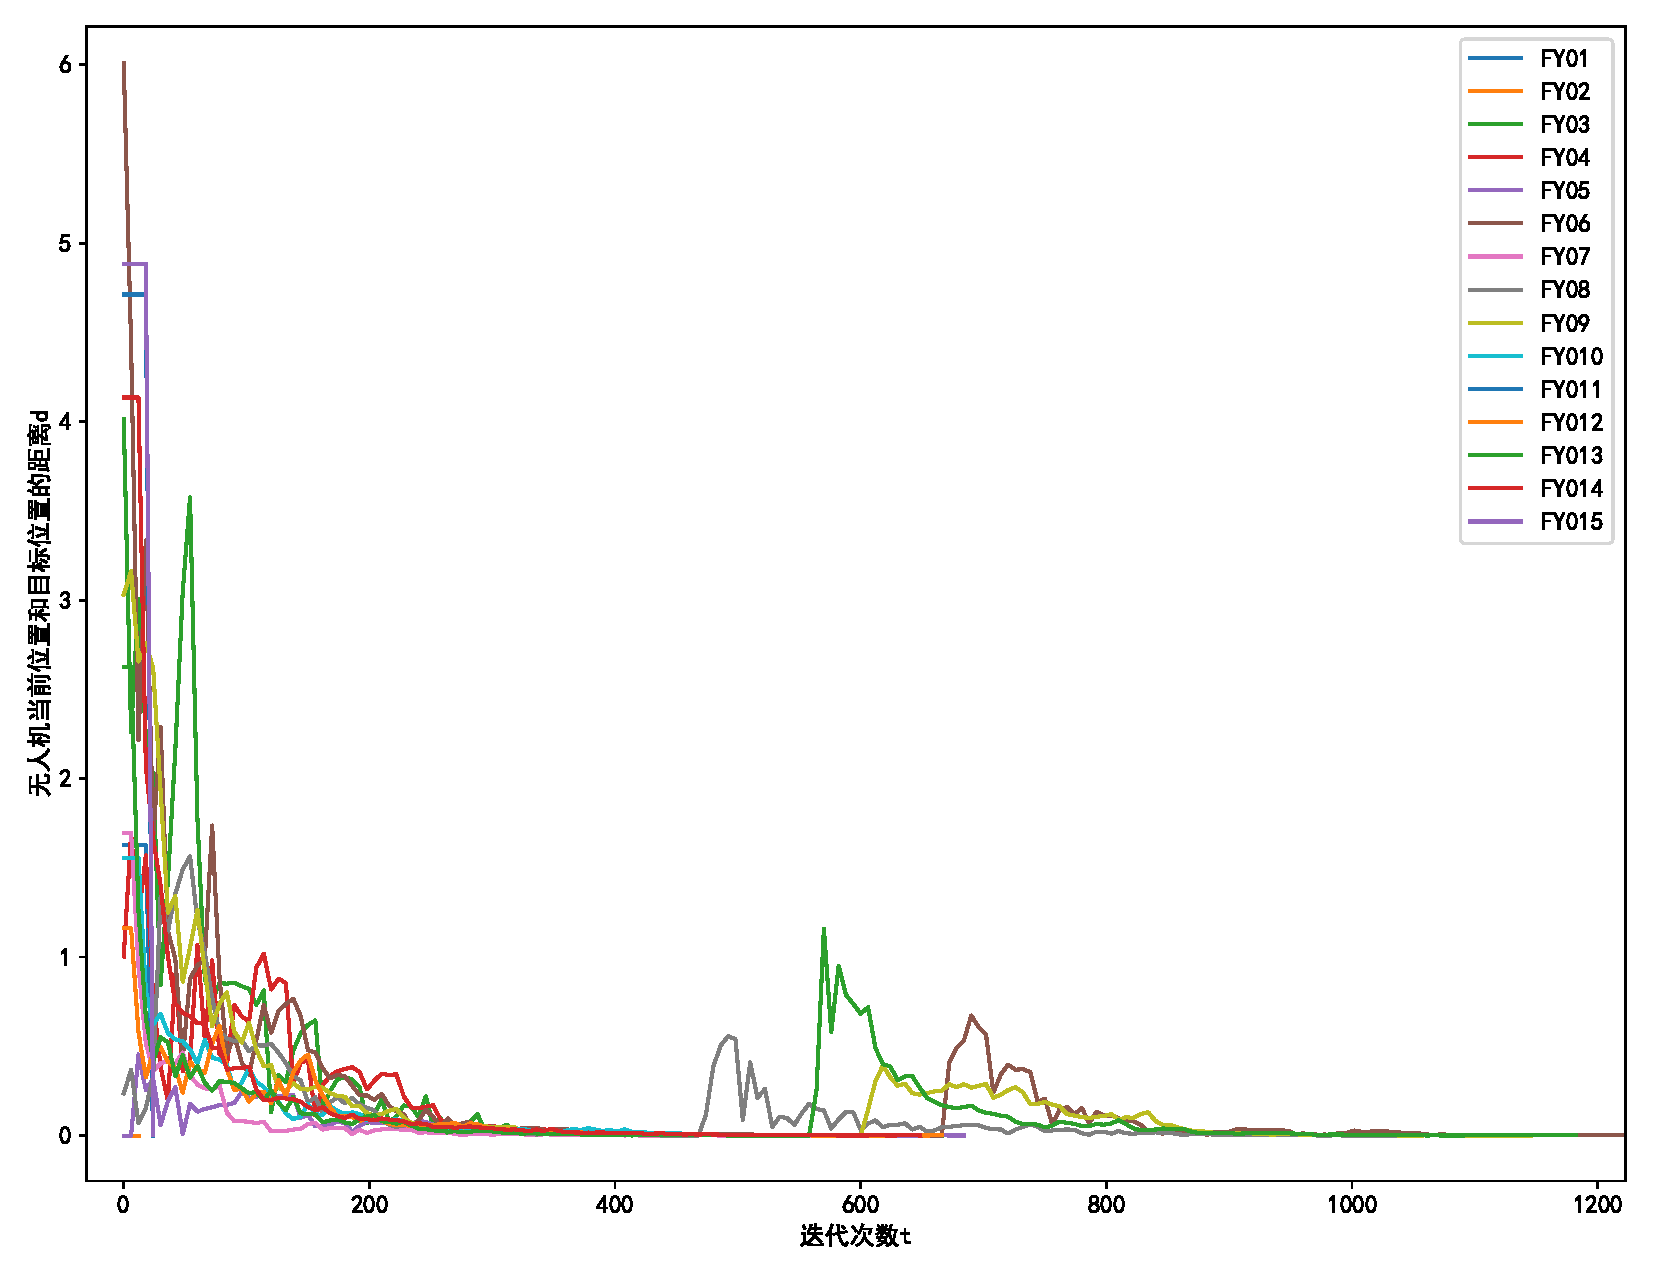
\includegraphics[width=0.7\linewidth]{figures/t15_0.pdf}
    \caption{每架无人机与其目标之间距离变化趋势}
    \label{fig:T15_Convergence}
\end{figure}
由上图可见,所有无人机与目标距离均收敛至0,成功调整至理想位置。



\subsection{可扩展性和效率分析}
该算法具有可扩展性和高效率:
对于无人机总数目$N$很大的情况,本算法依然能够生效。在每次调整中,只会用到圆心一架和圆周上六架共七架无人机;不难发现,对于由$N=\frac{k(k+1)}{2}$(上图中$N=15, k=5$)架无人机组成的等边三角形阵型,只需要$M=\frac{(k-3)(k-2)}{2}$次“七机圆形调整”和3三次角上调整就可以将所有无人机均调至理想状态。
由于每次“七机圆形调整”收敛所需的迭代次数是一个在固定值范围内小范围浮动的数,不妨设其均值为$T$,可以总结出,所有无人机都收敛至理想状态所需的迭代次数为
\begin{equation}
    T_{total} \approx MT = \frac{(k-3)(k-2)}{2} T \approx (N-3\sqrt{2N}) T = O(N)T
\end{equation}
可见总迭代次数仅随无人机总数目线性增加,且处理小规模问题和大规模问题时算法并无区别,从而证明了该算法的高效率和可扩展性。



\section{灵敏度分析}
\subsection{初始位置偏移量对收敛情况的影响}\label{startpos}

\begin{table}[H]
    \caption{初始位置偏移量不同程度的模拟值}\label{tab:sim} 
    \centering
    \begin{tabular}{cc|cc|cc}
        \toprule[1.5pt]
\multicolumn{2}{c}{\textbf{初始}} & \multicolumn{2}{c}{\textbf{中偏}} & \multicolumn{2}{c}{\textbf{高偏}} \\
        \midrule[1pt]
无人机编号   & 极坐标(m,   °)  & 无人机编号  & 极坐标(m,   °)   & 无人机编号  & 极坐标(m,   °)   \\
1       & (100, 0)     & 1      & (100, 0)      & 1      & (100, 0)      \\
2       & (100, 40)    & 2      & (125, 35.23)  & 2      & (129, 18.23)  \\
3       & (100, 80)    & 3      & (112, 71.27)  & 3      & (130, 59.27)  \\
4       & (100, 120)   & 4      & (87, 109.11)  & 4      & (79, 99.11)   \\
5       & (100, 160)   & 5      & (129, 166.48) & 5      & (129, 178.48) \\
6       & (100, 200)   & 6      & (72, 210.89)  & 6      & (72, 207.89)  \\
7       & (100, 240)   & 7      & (110, 229.56) & 7      & (125, 200.56) \\
8       & (100, 280)   & 8      & (94, 295.12)  & 8      & (79, 295.12)  \\
9       & (100, 320)   & 9      & (130, 330.02) & 9      & (130, 340.02) \\
        \bottomrule[1.5pt]
    \end{tabular}
\end{table}


对于与目标位置存在不同程度的偏移量的初始位置。在以下初始位置存在中高偏移量的设置中,算法最终都使全部无人机均收敛到了理想位置,体现了对初始位置很好的健壮性。
\begin{figure}[H]
    \centering
    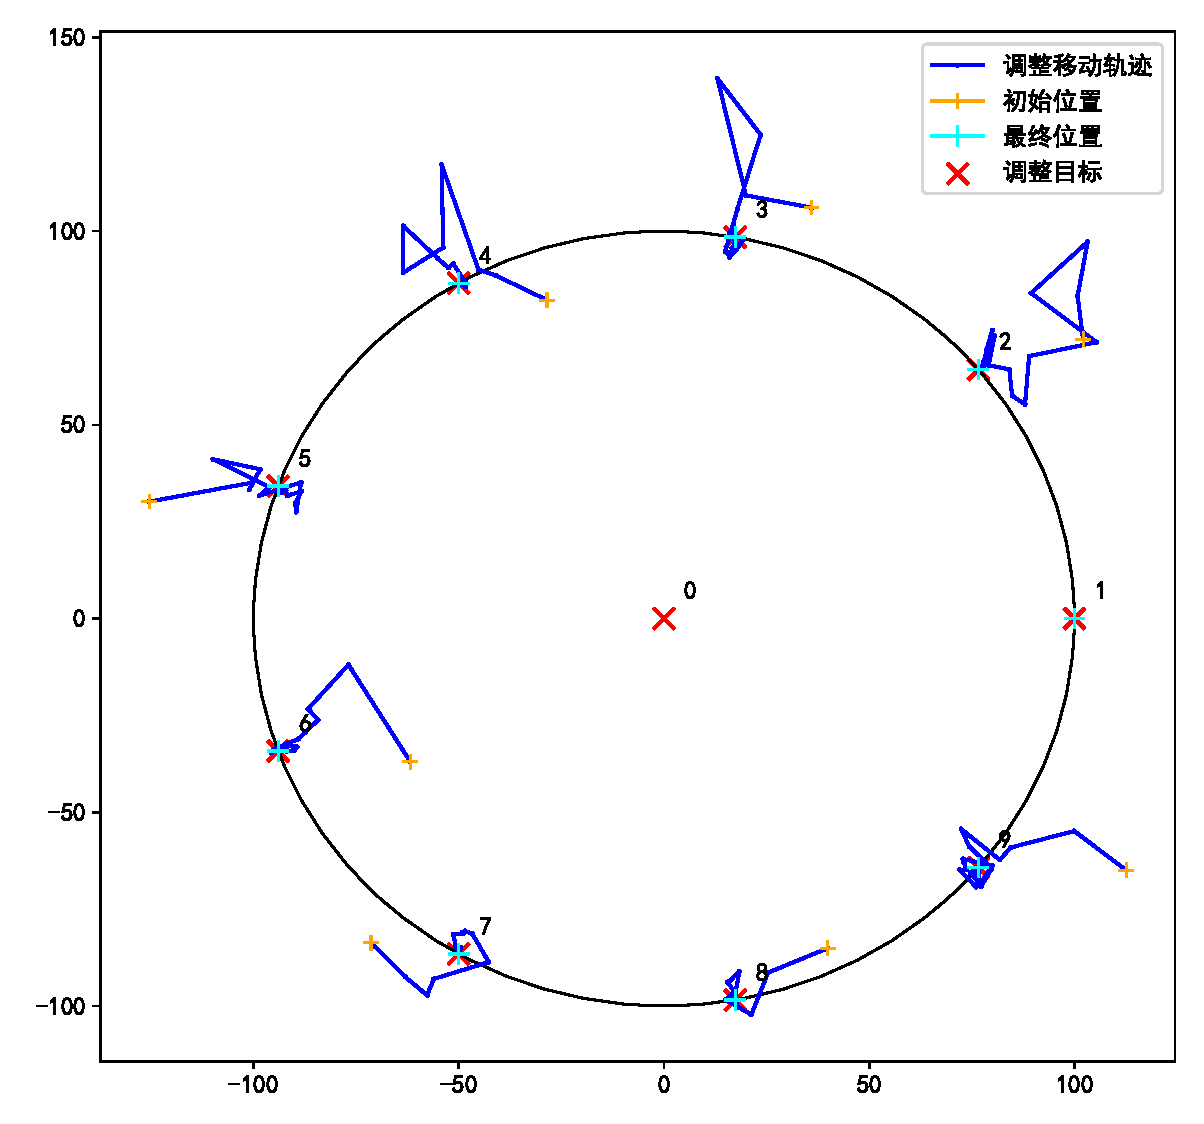
\includegraphics[width=0.7\linewidth]{figures/c9_noisy1.pdf}
    \caption{初始位置偏移量\textbf{中等}的无人机偏移量无人机移动轨迹}
    \label{fig:Circle9_1}
\end{figure}
\begin{figure}[H]
    \centering
    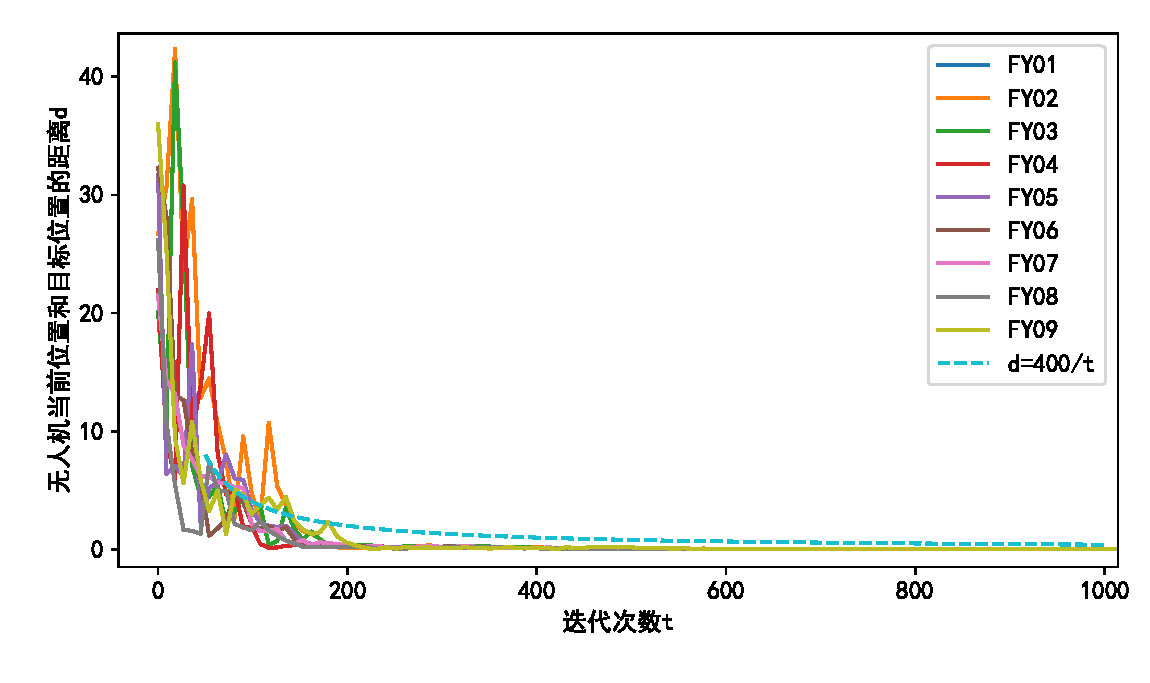
\includegraphics[width=0.9\linewidth]{figures/c9_noisy1_conv.pdf}
    \caption{初始位置偏移量\textbf{中等}的无人机与其目标之间距离变化趋势}
    \label{fig:Circle9_1_conv}
\end{figure}

\begin{figure}[H]
    \centering
    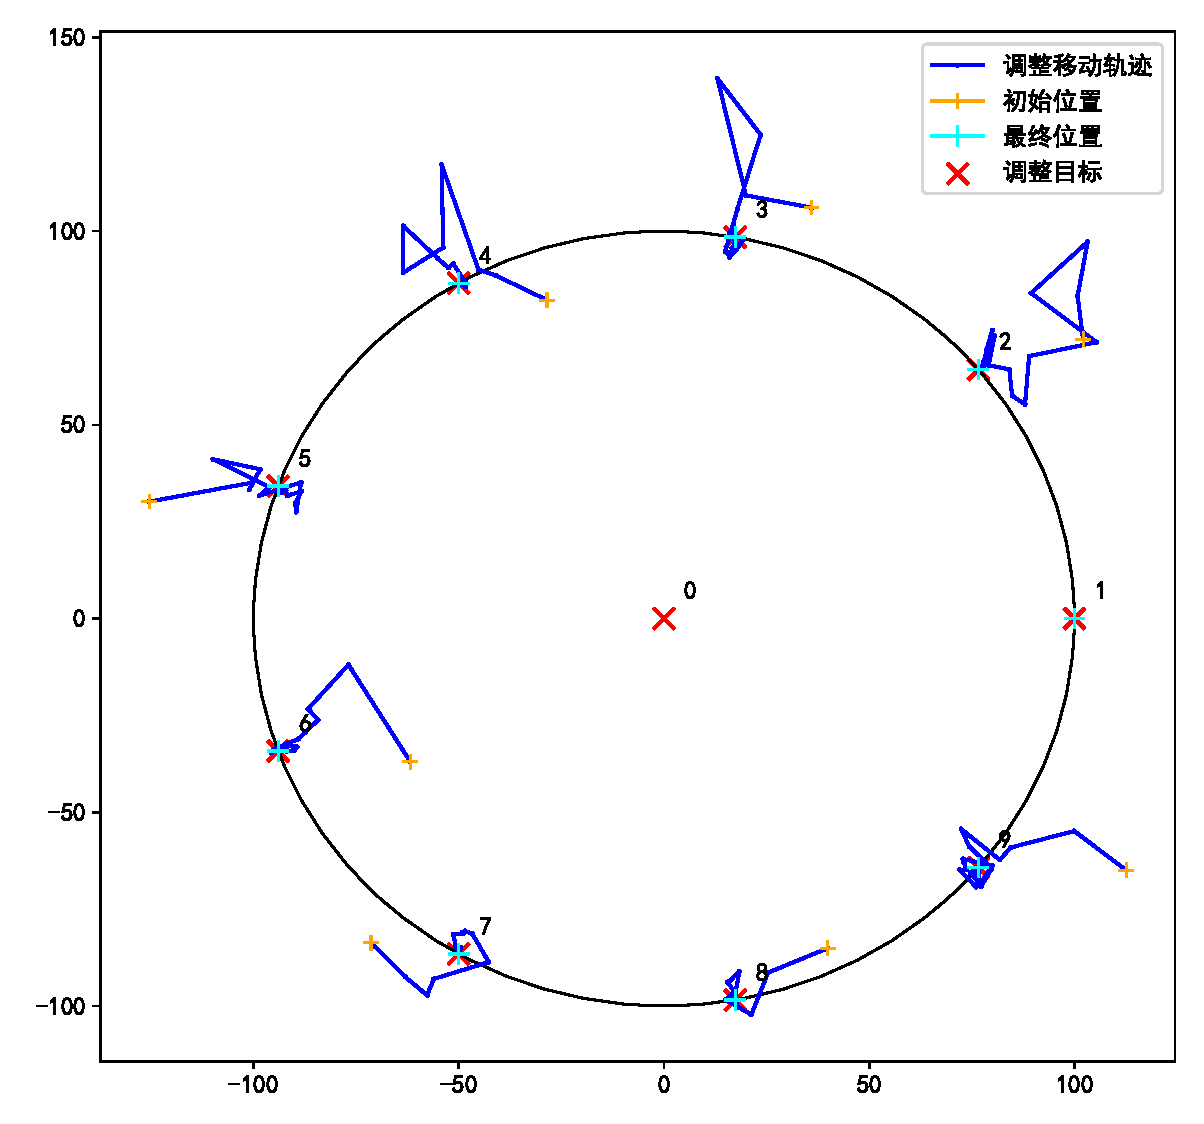
\includegraphics[width=0.7\linewidth]{figures/c9_noisy1.pdf}
    \caption{初始位置偏移量\textbf{高}的无人机偏移量无人机移动轨迹}
    \label{fig:Circle9_1}
\end{figure}
\begin{figure}[H]
    \centering
    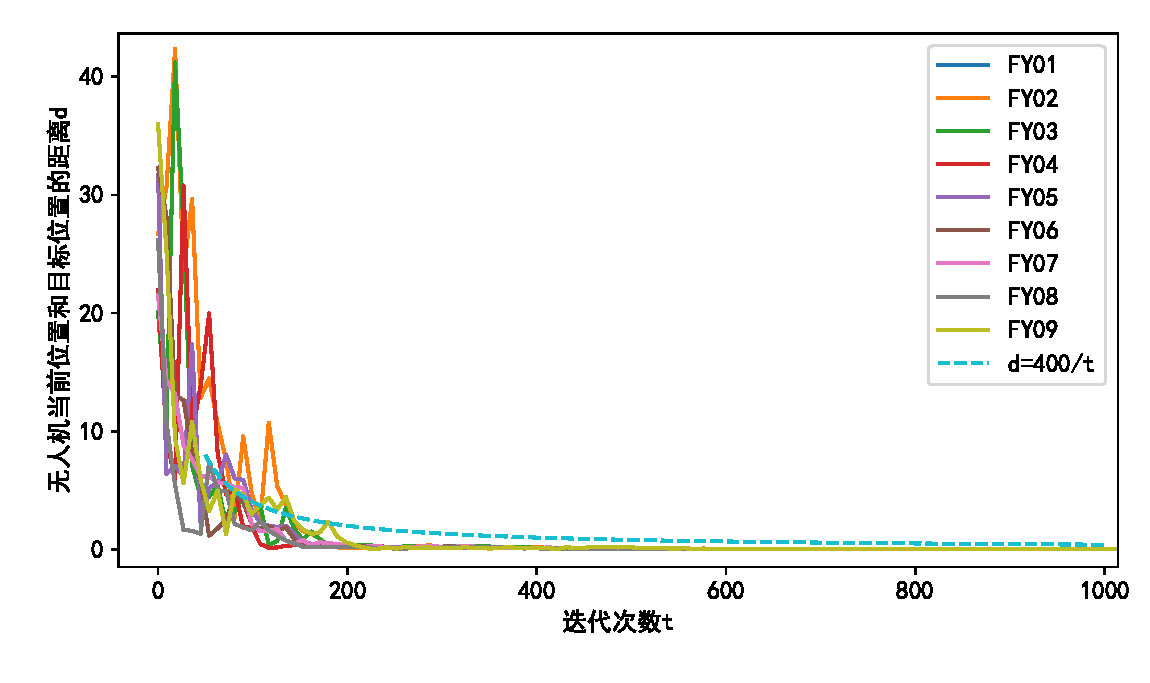
\includegraphics[width=0.9\linewidth]{figures/c9_noisy1_conv.pdf}
    \caption{初始位置偏移量\textit{高}的无人机偏移量无人机与其目标之间距离变化趋势}
    \label{fig:Circle9_1_conv}
\end{figure}

\subsection{学习率$\eta$对收敛情况的影响}
众所周知,梯度下降算法中的学习率会对结果的精度,收敛与否和收敛的速度产生巨大的影响。下面对三个不同的学习率进行实验,初始位置均采用\ref{startpos}中偏移量\textit{中等}的初始位置。

在图\ref{fig:Diff_eta}、\ref{fig:Diff_eta_conv}中,可以看到,在三个不同的学习率设置下,算法最终均收敛到理想位置。学习率较小时,算法收敛平稳,最终收敛效果更精确,移动轨迹较为平滑,但缺点是收敛速度较慢;学习率较大时,目标函数值震荡明显,最终收敛误差相对大,轨迹也非常曲折,但好处是收敛速度明显更快。在实际问题中需要根据需求进行学习率调整;但总体来说算法的收敛性对学习率$\eta$的健壮性较好。
\begin{figure}[H]
    \centering
    \begin{subfigure}{0.33\linewidth}
        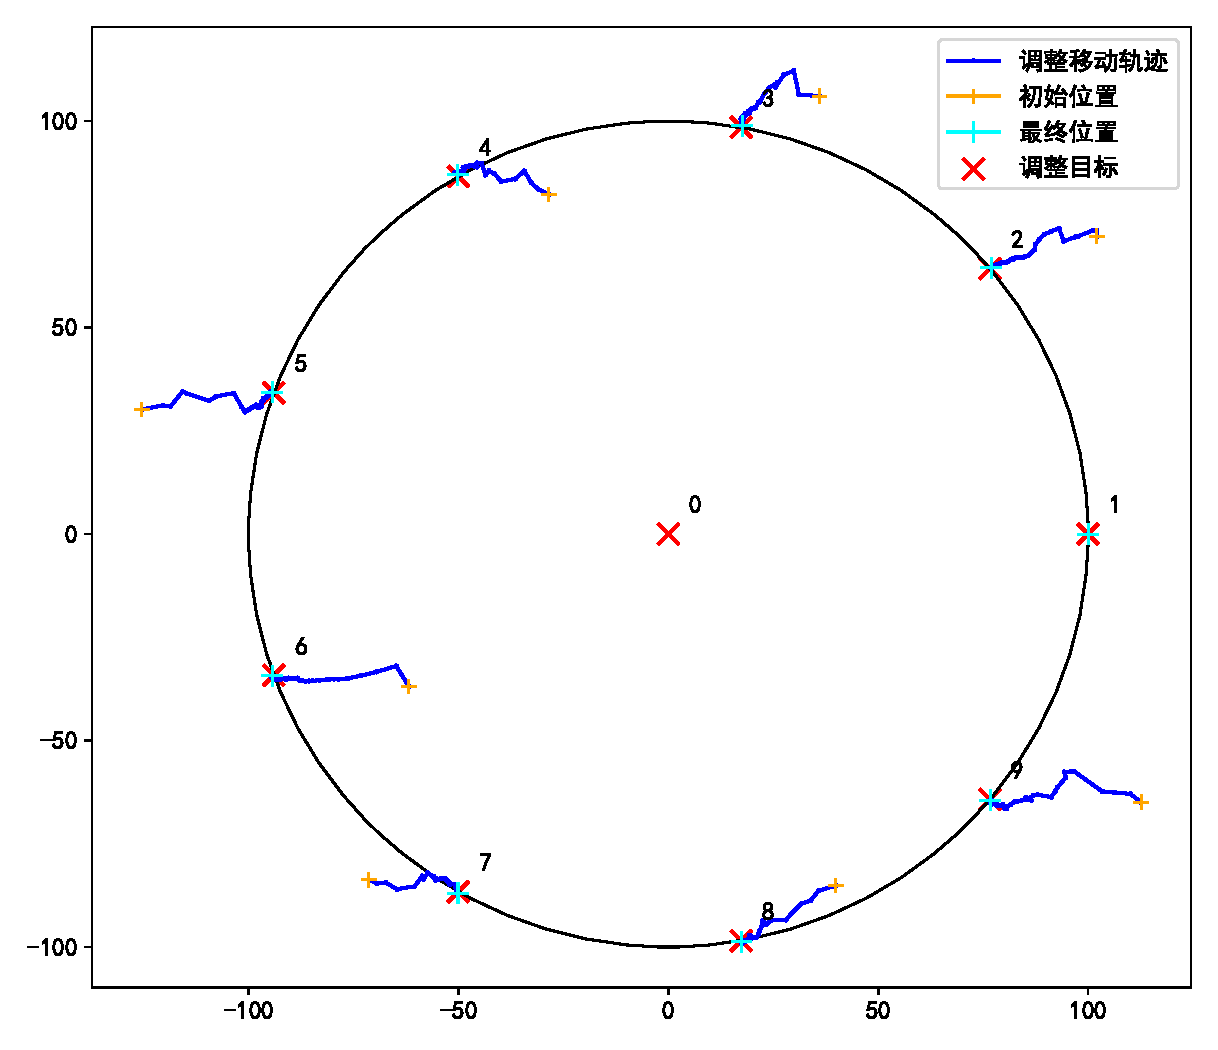
\includegraphics[width=1\linewidth]{figures/c9_lr0-1_.pdf}
        \caption{$\eta=0.1$}
    \end{subfigure}
    \begin{subfigure}{0.31\linewidth}
        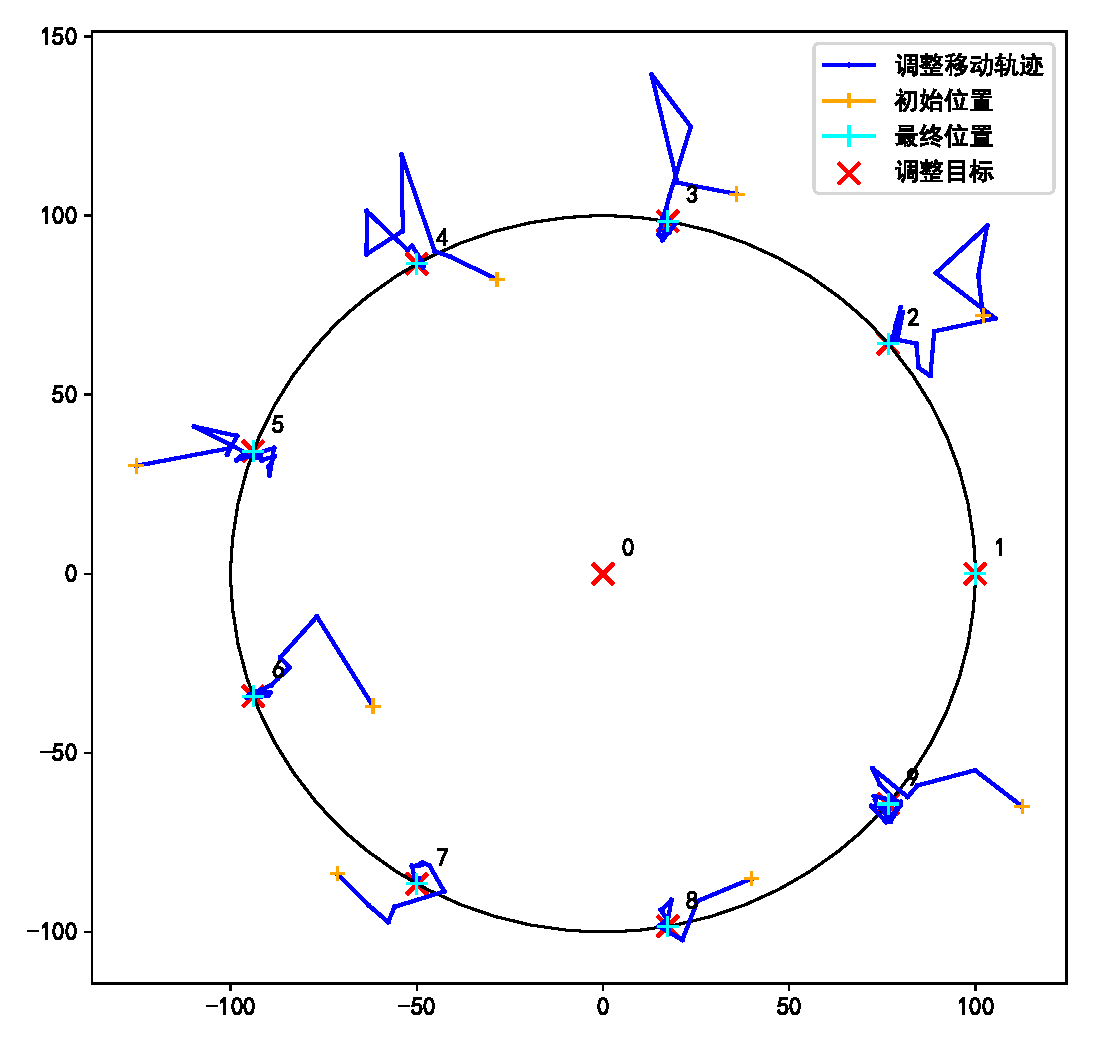
\includegraphics[width=1\linewidth]{figures/c9_lr0-5.pdf}
        \caption{$\eta=0.5$}
    \end{subfigure}
    \begin{subfigure}{0.32\linewidth}
        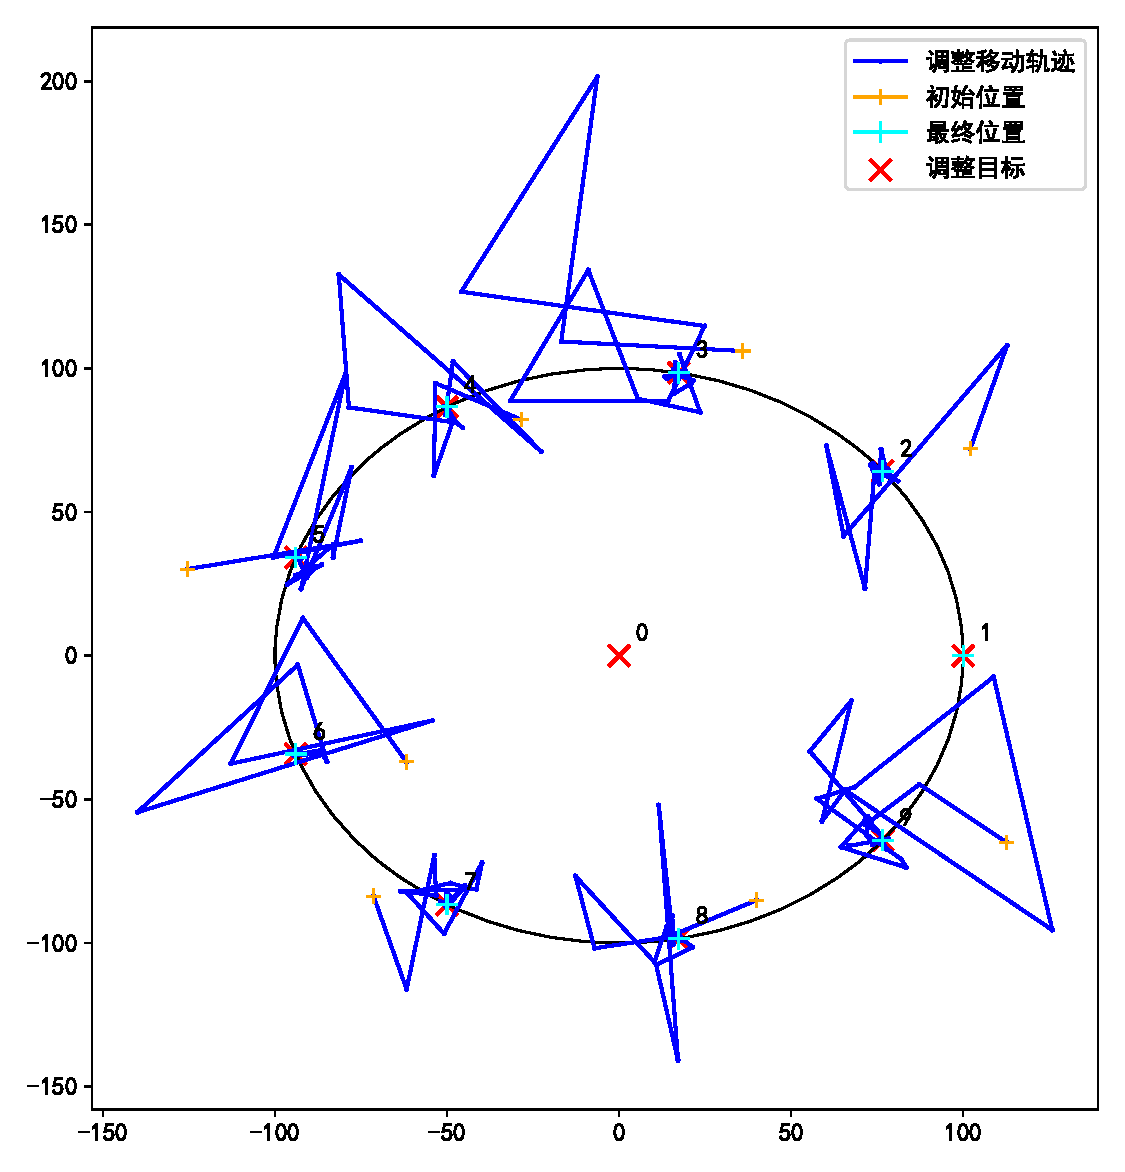
\includegraphics[width=1\linewidth]{figures/c9_lr1-0.pdf}
        \caption{$\eta=1.0$}
    \end{subfigure}
    \caption{不同学习率$\eta$对移动轨迹产生的影响}
    \label{fig:Diff_eta}
\end{figure}

\begin{figure}[H]
    \centering
    \begin{subfigure}{0.7\linewidth}
        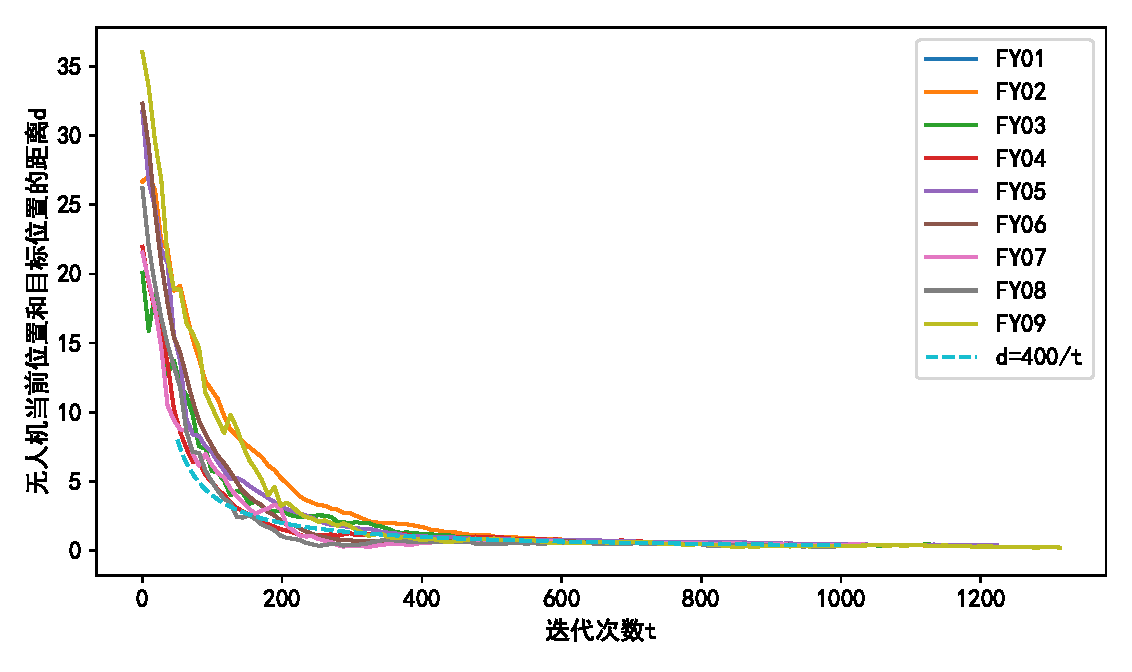
\includegraphics[width=1\linewidth]{figures/c9_lr0-1_conv.pdf}
        \caption{$\eta=0.1$}
    \end{subfigure}
    \begin{subfigure}{0.7\linewidth}
        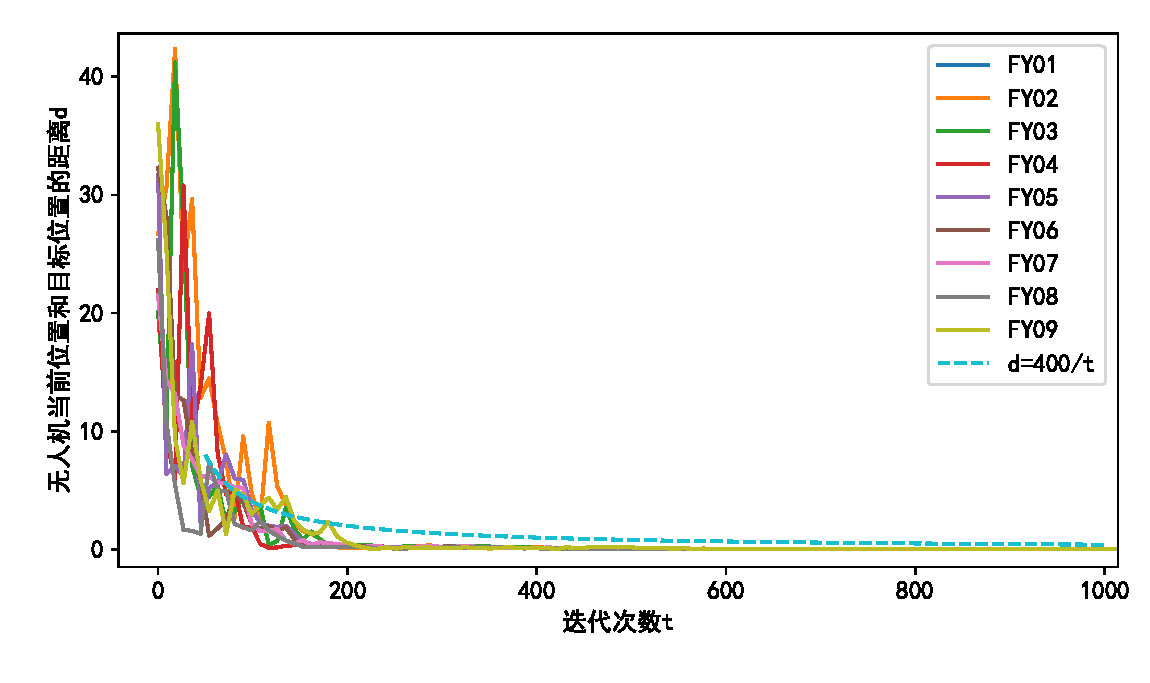
\includegraphics[width=1\linewidth]{figures/c9_noisy1_conv.pdf}
        \caption{$\eta=0.5$}
    \end{subfigure}
    \begin{subfigure}{0.7\linewidth}
        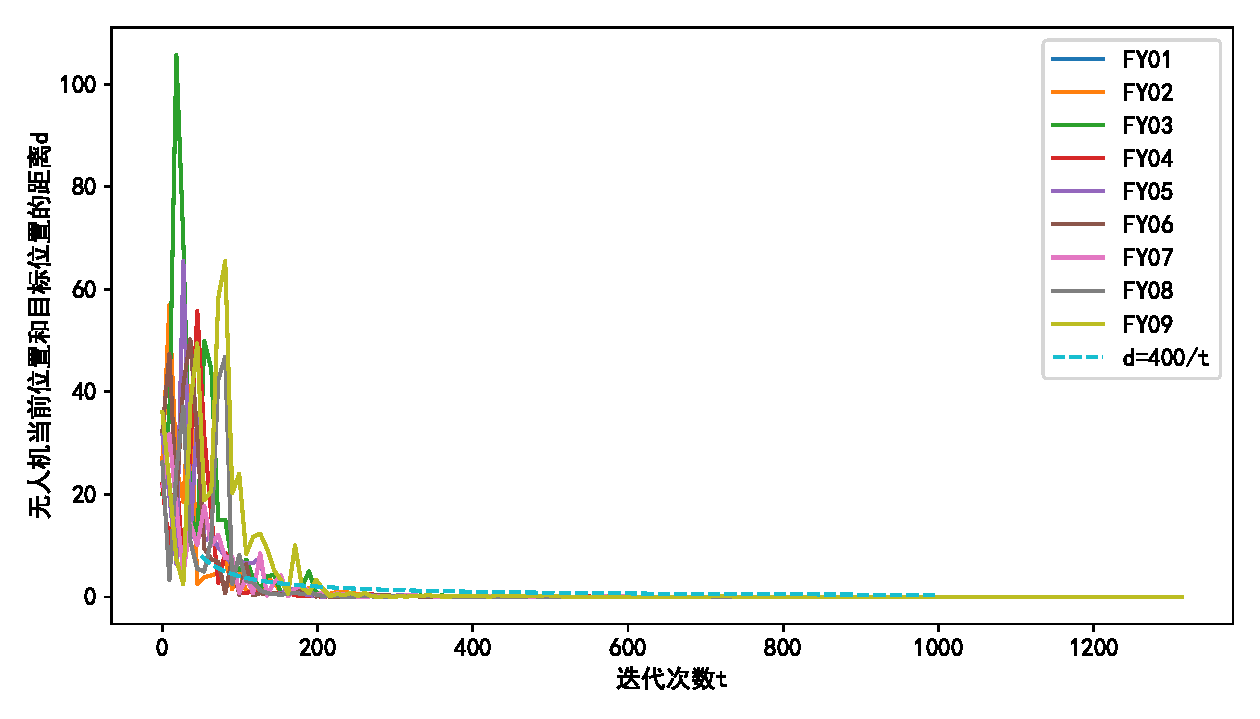
\includegraphics[width=1\linewidth]{figures/c9_lr1-0_conv.pdf}
        \caption{$\eta=1.0$}
    \end{subfigure}
    \caption{不同学习率$\eta$对收敛速度产生的影响}
    \label{fig:Diff_eta_conv}
\end{figure}


\section{模型评价}

\subsection{模型优点}

\begin{enumerate}[{1)}]
    \item 本文在解决目标问题时,考虑了相对位置的四种不同情况,分析全面;同时构造的模型形式简洁精炼,易于理解和数值计算求解;
    \item 本文建模中接收信号无人机只接收了方向信息,相比于其他研究包含了距离和方向两类信息,本文的模型在实际无人机系统中中所需的传感器数量少,可带来成本低、适用范围广等优势;
    \item 本文所采用的算法鲁棒性较高,无论是无人机数目较多,还是在无人机初始位置偏离预设位置较远或是不同学习率,算法均能有效地将无人机定位和调整至预设目标位置。
\end{enumerate}

\subsection{模型不足}

\begin{enumerate}[{1)}]
    \item 本文只考虑了二维平面的情况,而在实际情况中三维更为常见;
    \item 模型中的学习率的改变虽然会带来优点(3)的好处,但同时增加了方案的不确定性:不同的学习率可能造成收敛速度的改变和无人机调整过程中出现不同程度的无规律运动。在运用本模型实际求解的过程中,使用方宜改变学习率多次运行求解过程,选取较好方案作为最终解,或将学习率根据目标函数值情况动态调整,限于篇幅本文不再讨论。


\end{enumerate}

\subsection{模型可推广性分析}

\begin{enumerate}[{1)}]
    \item 除了文中所讨论的圆形和锥形的情况,该模型还可推广至有高度对称性的编队情况。只要获得预设好的编队坐标,便可以实施类似的定位模型,并且在有偏差的时候根据算法进行调整;
    \item 该模型可以推广至三维情况,在讨论的过程中,需要将原来模型的平面角改为方位角,考虑更多种情况。模型经此推广之后可以更加符合现实生活的场景;
    \item 该模型还可以应用于军事战场,卫星排布等领域,可以通过该模型通过预设好的相对位置将相关事物基本回到指定位置。
\end{enumerate}











\newpage
%----------------------------------------------------------------------------------------
% Bibliography
%----------------------------------------------------------------------------------------
% \newpage % Includes a new page

\pagenumbering{roman} % Changes page numbering to roman page numbers
%\bibliography{literature}

\bibliography{literature.bib} % Add the filename of your bibliography
\bibliographystyle{IEEEtran} % Defines your bibliography style

% For citing, please see this sheet: http://merkel.texture.rocks/Latex/natbib.php




\newpage
%附录
\begin{appendices}

\section{圆形编队调整方案——python源代码}

\begin{lstlisting}[language=python]
import matplotlib.pyplot as plt
import matplotlib.font_manager as fm
import numpy as np
import math
import random
plt.rcParams['font.family']=['SimHei']
plt.rcParams.update({'font.size': 12})
plt.rcParams['axes.unicode_minus'] = False

CENTER = np.array((0, 0))
R = 100

COORDS = [(0,0),
          (100,0),
          (98,40.10),
          (112,80.21),
          (105,119.75),
          (98,159.86),
          (112,199.96),
          (105,240.07),
          (98,280.17),
          (112,320.28)]

COORDS_2 = [
    (0,0),
    (100, 0),
    (125, 35.23),
    (112, 71.27),
    (87, 109.11),
    (129, 166.48),
    (72, 210.89),
    (110, 229.56),
    (94, 295.12),
    (130, 330.02)]
def rad2dec(x): # 极坐标转为直角坐标
    r, theta = x[0], x[1]
    return np.array((r*np.cos(theta), r*np.sin(theta)))

def dec2rad(v):
    x, y = v[0], v[1]
    r = np.sqrt(x * x + y * y), 
    theta = np.arctan2(y, x)
    if theta < 0:
        theta += 2 * np.pi
    return np.array((r, theta), dtype=object)


def plot_dots(lst, mk=False, **kwargs):
    x = [v[0] for v in lst]
    y = [v[1] for v in lst]
    plt.scatter(x, y, **kwargs)
    if mk:
        marks = [str(i) for i in range(0, len(x))]
        for i in range(len(x)):
            plt.annotate(marks[i], xy = (x[i], y[i]), xytext = (x[i] + 5, y[i] + 5))

def calc_angle(v1, v2):
    cos_angle = v1.dot(v2) / (np.linalg.norm(v1) * np.linalg.norm(v2))
    theta = np.arccos(cos_angle)
    if theta < 0:
        theta += np.pi
    return theta

def calc_pos(i, j, k, a1, a2, b1, b2):
    # case 1
    assert k != 0, "k should be 1~9"
    # print(math.degrees(a1), math.degrees(a2), math.degrees(b1), math.degrees(b2),sep=',')
    b = b2 - b1
    yl0 = np.sin(a1)*np.sin(a2)
    yr0 = np.sin(b + a2)*np.sin(a1)
    yr1 = np.sin(b - a2)*np.sin(a1)
    xl0 = np.cos(a1)*np.sin(a2)
    xr0 = np.cos(b+a2)*np.sin(a1)
    xr1 = np.cos(b-a2)*np.sin(a1)
    
    is_inside = i < k < j
    # gt_180_cnt = 0
    if np.abs(j - k) > 4.5:
        is_inside = not is_inside
        # gt_180_cnt += 1
    if np.abs(k - i) > 4.5:
        is_inside = not is_inside
        # gt_180_cnt += 1
    
    up_down = k in ((i)%9+1, (i+1)%9+1, (i+2)%9+1, (i+3)%9+1)
    # if gt_180_cnt == 2:
    #     up_down = not up_down
    
    if up_down:
        yl, xl = yl0, xl0
        if is_inside:
            # print("case 1")
            yr, xr = -yr0, xr0
        else:
            yr, xr = yr1, -xr1
            # print("case 2")
        kappa = (yl + yr) / (xl + xr)
        theta_hat = -np.arctan(kappa) if kappa <= 0 else np.pi - np.arctan(kappa)
        d =  R * np.sin(theta_hat + a1) / np.sin(a1)
        theta = theta_hat + b1
        if theta < 0:
            theta += 2 * np.pi
    else:
        yl, xl = yl0, -xl0
        if is_inside:
            yr, xr = yr1, -xr1
            # print("case 3")
        else:
            yr, xr = -yr0, xr0
            # print("case 4")
        kappa = (yl + yr) / (xl + xr)
        # print(f"kappa:{kappa}")
        theta_hat = np.pi + np.arctan(kappa) if kappa <= 0 else np.arctan(kappa)
        d =  R * np.sin(theta_hat + a1) / np.sin(a1)
        theta = b1 - theta_hat
        if theta < 0:
            theta += 2 * np.pi
    # y = (np.sin(a1-b1)*np.sin(a2) - np.sin(a2+b2)*np.sin(a1))
    # x = np.cos(a1-b1)*np.sin(a2) + np.cos(a2+b2)*np.sin(a1)
    
    # print("theta:",theta)
    return d, theta
    
class DroneGroup:
    def __init__(self, coords) -> None:
        self.N = len(coords) - 1
        self.pos = [rad2dec((c[0], math.radians(c[1]))) for c in coords] # 极坐标
        self.target = [np.zeros(2)] + [rad2dec((R, math.radians(w))) for w in range(0, 360, 360//self.N)]
    
    def calc_delta(self, i, j, k, ref1, ref2, ref0=CENTER,debug=False):
        p_real = self.pos[k]
        p_tgt = self.target[k]
        a1 = calc_angle(ref0 - p_real, ref1 - p_real)
        a2 = calc_angle(ref0 - p_real, ref2 - p_real)
        b1 = dec2rad(ref1)[1]
        b2 = dec2rad(ref2)[1]
        
        r_, theta_ = calc_pos(i, j, k, a1, a2, b1, b2)
        # if debug:
        #     print(f"r_:{r_}, θ: {math.degrees(theta_)}")
        p_est = rad2dec((r_, theta_)) # 估计的坐标(笛卡尔)
        if debug:
            print(f"Estimated: {p_est}, actual: {p_real}, target: {p_tgt}")
        delta = p_tgt - p_est
        if np.linalg.norm(p_est - p_tgt) > 1e2:
            raise ValueError("Prediction Error!")
        return delta
    
    # def adjust(self, k): # 调整k号无人机
    #     tot_delta = np.zeros(2)
    #     cnt = 0
    #     for i in range(1, self.N + 1):
    #         for j in range(1, self.N + 1):
    #             if i < j and i != k and j != k:
    #                 delta = self.calc_delta(self.pos[k], self.pos[i], self.pos[j])
    #                 tot_delta += delta
    #                 cnt += 1
    #     avg_delta = tot_delta / cnt
    #     return avg_delta
    
    def adjust_random(self, rounds, lr=0.5):
        REFPT = 1
        dots_x = [[] for _ in range(10)]
        dots_y = [[] for _ in range(10)]
        for idx in range(1, 10):
            dots_x[idx].append(self.pos[idx][0])
            dots_y[idx].append(self.pos[idx][1])
        tmp = list(range(1,10))
        while rounds > 0:
            rounds -= 1
            random.shuffle(tmp)
            i, j, k = tmp[0], tmp[1], tmp[2]
            if k == REFPT:
                rounds += 1
                continue
            if i > j:
                i, j = j, i
            delta = self.calc_delta(i, j, k, self.pos[i], self.pos[j], debug=True)
            
            print(f"delta:{delta}")
            # 更新
            DG.pos[k] += lr * delta
            
            dots_x[k].append(self.pos[k][0])
            dots_y[k].append(self.pos[k][1])
        
        return dots_x, dots_y
            
if __name__ == "__main__":
    
    # random.seed(114514)
    # random.seed(1919)
    random.seed(810)
    
    DG = DroneGroup(COORDS)
    print(DG.pos)
    
    draw_circle = plt.Circle(CENTER, R, fill=False)
    plt.gcf().gca().add_artist(draw_circle)
    # plot_dots(DG.pos, color='blue')
    plot_dots(DG.target, mk=True, marker='x',color='red',s=100,label='调整目标')
    
    EPOCHS = 1000
    
    dots_x, dots_y = DG.adjust_random(EPOCHS)
    # print(dots_x, dots_y)
    for i in range(1, 10):
        label1 = '调整移动轨迹' if i == 1 else None 
        label2 = label='初始位置'if i ==1 else None
        label3 = label='最终位置'if i ==1 else None
        plt.plot(dots_x[i], dots_y[i], marker='.', markersize=2, color='blue', label=label1)
        plt.plot(dots_x[i][0], dots_y[i][0], marker='+', markersize=7, color='orange', label=label2)
        plt.plot(dots_x[i][-1], dots_y[i][-1], marker='+', markersize=10, color='cyan', label=label3)
        
    # print("t", DG.target[3])
    # k = 9
    # for i in range(1,10):
    #     for j in range(1, 10):
    #         if i < j and i != k and j != k: 
    #             print(i, j)
    #             print(DG.calc_delta(i, j, k, DG.target[i], DG.target[j],debug=True))
    # plt.legend()
    plt.show()
    
    plt.clf()
    
    n = 9
    for i in range(1, n+1):
        ep = len(dots_x[i])
        t = np.array(list(range(ep))) * n
        print(DG.target[i])
        print(np.array((dots_x[i][-1],dots_y[i][-1])))
        dist = [np.linalg.norm(np.array((dots_x[i][j],dots_y[i][j])) - DG.target[i]) for j in range(ep)]
        plt.plot(t, dist, label=f"FY0{i}")    
    
    t = np.array(list(range(50, EPOCHS)))
    plt.plot(t, 400 * 1/(t), '--', label='d=400/t', )
    
    plt.xlabel("迭代次数t")
    plt.ylabel("无人机当前位置和目标位置的距离d")
    plt.legend()
    plt.show()
    # print(DG.target)
 \end{lstlisting}

\section{锥形编队调整方案——python源代码}

\begin{lstlisting}[language=python]
import matplotlib.pyplot as plt
import matplotlib.font_manager as fm
import numpy as np
import math
import random
plt.rcParams['font.family']=['SimHei']
plt.rcParams.update({'font.size': 12})
plt.rcParams['axes.unicode_minus'] = False

CENTER = np.array((0, 0))
R = 50
NIL = -1

TARGET_COORDS = [  (0, 0), # point zero
            (86.60, 330),
            (50, 0),
            (50, 300),
            (50, 60),
            (0, 0),
            (50, 240),
            (86.6025, 90),
            (50, 120),
            (50, 180),
            (86.6025, 210),
            (132.2875, 100.893),
            (100, 120),
            (86.6025, 150),
            (100, 180),
            (132.2875, 199.107)
            ]

COORDS = [  (0, 0), # point zero
            (85, 330.20),
            (50, 0),
            (54, 299.61),
            (49, 60.10),
            (0, 0),
            (56, 240.41),
            (85, 89.63),
            (50, 120.27),
            (53, 180.48),
            (88, 209.55),
            (137, 100.87),
            (99, 120.34),
            (84, 150.23),
            (104, 179.41),
            (137, 198.56)
]

COORDS_2 = [
            (0,0), 
            (80, 333.20),
            (50, 0),
            (63, 297.61),
            (41, 63.10),
            (0, 0),
            (61, 243.41),
            (80, 84.63),
            (54, 122.27),
            (63, 184.48),
            (91, 207.55),
            (147, 100.87),
            (92, 125.34),
            (80, 155.23),
            (107, 176.41),
            (141, 196.56),

]

def rad2dec(x): # 极坐标转为直角坐标
    r, theta = x[0], x[1]
    return np.array((r*np.cos(theta), r*np.sin(theta)))

def dec2rad(v):
    x, y = v[0], v[1]
    r = np.sqrt(x * x + y * y), 
    theta = np.arctan2(y, x)
    if theta < 0:
        theta += 2 * np.pi
    return np.array((r, theta), dtype=object)


def plot_dots(lst, mk=False, mk_offset=0, **kwargs):
    x = [v[0] for v in lst]
    y = [v[1] for v in lst]
    plt.scatter(x, y, **kwargs)
    if mk:
        marks = [str(i+mk_offset) for i in range(0, len(x))]
        for i in range(len(x)):
            plt.annotate(marks[i], xy = (x[i], y[i]), xytext = (x[i]+0.5, y[i]+0.5))

def calc_angle(v1, v2):
    cos_angle = v1.dot(v2) / (np.linalg.norm(v1) * np.linalg.norm(v2))
    theta = np.arccos(cos_angle)
    if theta < 0:
        theta += np.pi
    return theta

def calc_pos(i, j, k, a1, a2, b1, b2):
    print(f"i_:{i}, j_:{j}, k_:{k}")
    # case 1
    # assert k != 0, "k should be 1~9"
    # print(math.degrees(a1), math.degrees(a2), math.degrees(b1), math.degrees(b2),sep=',')
    b = b2 - b1
    yl0 = np.sin(a1)*np.sin(a2)
    yr0 = np.sin(b + a2)*np.sin(a1)
    yr1 = np.sin(b - a2)*np.sin(a1)
    xl0 = np.cos(a1)*np.sin(a2)
    xr0 = np.cos(b+a2)*np.sin(a1)
    xr1 = np.cos(b-a2)*np.sin(a1)
    
    is_inside = i < k < j
    # gt_180_cnt = 0
    if np.abs(j - k) > 3:
        is_inside = not is_inside
        # gt_180_cnt += 1
    if np.abs(k - i) > 3:
        is_inside = not is_inside
        # gt_180_cnt += 1
    
    up_down = k in ((i)%6+1, (i+1)%6+1)
    # if gt_180_cnt == 2:
    #     up_down = not up_down
    
    if up_down:
        yl, xl = yl0, xl0
        if is_inside:
            print("case 1")
            yr, xr = -yr0, xr0
        else:
            yr, xr = yr1, -xr1
            print("case 2")
        kappa = (yl + yr) / (xl + xr)
        print(f"k:{kappa}")
        theta_hat = -np.arctan(kappa) if kappa <= 0 else np.pi - np.arctan(kappa)
        print(f"thetahat{math.degrees(theta_hat)}")
        d =  R * np.sin(theta_hat + a1) / np.sin(a1)
        theta = theta_hat + b1
        if theta < 0:
            theta += 2 * np.pi
    else:
        yl, xl = yl0, -xl0
        if is_inside:
            yr, xr = yr1, -xr1
            print("case 3")
        else:
            yr, xr = -yr0, xr0
            print("case 4")
        kappa = (yl + yr) / (xl + xr)
        # print(f"kappa:{kappa}")
        theta_hat = np.pi + np.arctan(kappa) if kappa <= 0 else np.arctan(kappa)
        d =  R * np.sin(theta_hat + a1) / np.sin(a1)
        theta = b1 - theta_hat
        if theta < 0:
            theta += 2 * np.pi
    # y = (np.sin(a1-b1)*np.sin(a2) - np.sin(a2+b2)*np.sin(a1))
    # x = np.cos(a1-b1)*np.sin(a2) + np.cos(a2+b2)*np.sin(a1)
    
    # print("theta:",theta)
    return d, theta
    
class DroneGroupTri:
    def __init__(self, coords_target, coords) -> None:
        self.N = len(coords) - 1
        self.pos = [rad2dec((c[0], math.radians(c[1]))) for c in coords] # 极坐标
        self.target = [rad2dec((c[0], math.radians(c[1]))) for c in coords_target]
    
    def calc_delta(self, i, j, k, ref1, ref2, ref0, mapping, debug=False):
        print(i,j,k)
        p_real = self.pos[k]
        p_tgt = self.target[k]
        a1 = calc_angle(ref0 - p_real, ref1 - p_real)
        a2 = calc_angle(ref0 - p_real, ref2 - p_real)
        b1 = dec2rad(ref1 - ref0)[1]
        b2 = dec2rad(ref2 - ref0)[1]
        print(math.degrees(a1), math.degrees(a2), math.degrees(b1), math.degrees(b2),sep=',')
        i_, j_, k_ = mapping[i], mapping[j], mapping[k]
        r_, theta_ = calc_pos(i_, j_, k_, a1, a2, b1, b2)
        # if debug:
        #     print(f"r_:{r_}, θ: {math.degrees(theta_)}")
        p_est = rad2dec((r_, theta_)) + ref0 # 估计的坐标(笛卡尔)
        if debug:
            print(f"r_:{r_}, theta_:{math.degrees(theta_)}")
            print(f"Estimated: {p_est}, actual: {p_real}, target: {p_tgt}")
        delta = p_tgt - p_est
        if np.linalg.norm(delta) > 2e1:
            raise ValueError("Prediction Error!")
        return delta
    
    def one_hex(self, rounds, center, ref, around, lr, color, has_legend=False):
        mapping = dict()
        for i in range(6):
            mapping[around[i]] = i + 1
        dots_x, dots_y = self.adjust_random(rounds, center, ref, around, mapping, lr)
        # for i in range(1, DG.N+1):
        #     plt.plot(dots_x[i], dots_y[i], marker='.', color=color, markersize=0.5)
        #     # plt.plot(dots_x[i][-1], dots_y[i][-1], marker='*', color='cyan')
        for i in range(1, self.N+1):
            label1 = '调整移动轨迹' if i == 1 and has_legend else None 
            label2 = '初始位置' if i ==1 and has_legend else None
            label3 = '最终位置' if i ==1 and has_legend else None
            plt.plot(dots_x[i], dots_y[i], marker='.', markersize=2, color='blue', label=label1)
            plt.plot(dots_x[i][0], dots_y[i][0], marker='+', markersize=7, color='orange', label=label2)
            plt.plot(dots_x[i][-1], dots_y[i][-1], marker='+', markersize=10, color='cyan', label=label3)
        return dots_x, dots_y
    
        
    def traingle_adjust(self, rounds, lr=0.5):
        center = 5
        around = [2, 4, 8, 9, 6, 3]
        ref = 2
        
        
        dots_x, dots_y = self.one_hex(rounds, center, ref, around, lr, color='blue')
        X, Y = dots_x, dots_y
        # done = input("done!------------------------------------")
        
        center = 8
        around = [4, 7, 12, 13, 9, 5]
        ref = 4
        dots_x, dots_y = self.one_hex(rounds, center, ref, around, lr, color='green')
        for i in range(1, self.N+1):
            X[i] += dots_x[i]
            Y[i] += dots_y[i]
        
        center = 9
        around = [5, 8, 13, 14, 10, 6]
        ref = 5
        dots_x, dots_y = self.one_hex(rounds, center, ref, around, lr, color='purple', has_legend=True)
        for i in range(1, self.N+1):
            X[i] += dots_x[i]
            Y[i] += dots_y[i]
        # 调整三个角上的
        # k 是三角形角上的点
        def adjust_angle(i, j, k, center, mapping, color):
            delta = self.calc_delta(i, j, k, self.pos[i], self.pos[j], ref0=self.pos[center], mapping=mapping, debug=True)
            print(delta)
            self.pos[k] += 1.0 * delta
            dots_x[k].append(self.pos[k][0])
            dots_y[k].append(self.pos[k][1])
            plt.plot(dots_x[k], dots_y[k], marker='.', color=color, markersize=0.5)
        
        # adjust 15
        i, j, k = 9, 14, 15
        center = 10
        mapping = {6:1, 9:2, 14:3, 15:4}
        if mapping[i] > mapping[j]:
            i, j = j, i
        adjust_angle(i, j, k, center, mapping, color='pink')
        X[k] += dots_x[k]
        Y[k] += dots_y[k]
        
        # adjust 11
        i, j, k = 8, 7, 11
        center = 12
        mapping = {7:1, 11:2, 13:5, 8:6}
        if mapping[i] > mapping[j]:
            i, j = j, i
        adjust_angle(i, j, k, center, mapping, color='pink')
        X[k] += dots_x[k]
        Y[k] += dots_y[k]
        
        # adjust 1
        i, j, k = 2, 5, 1
        center = 3
        mapping = {1:1, 2:2, 5:3, 6:4}
        if mapping[i] > mapping[j]:
            i, j = j, i
        adjust_angle(i, j, k, center, mapping, color='pink')
        X[k] += dots_x[k]
        Y[k] += dots_y[k]
        
        
        for i in range(1, self.N+1):
            plt.plot(dots_x[i][-1], dots_y[i][-1], marker='*', color='cyan')   
        
        plt.legend()
        plt.show()
        
        plt.clf()
        
        n = self.N
        for i in range(1, n+1):
            ep = len(X[i])
            t = np.array(list(range(ep))) * 6
            print(DG.target[i])
            print(np.array((X[i][-1],Y[i][-1])))
            dist = [np.linalg.norm(np.array((X[i][j],Y[i][j])) - DG.target[i]) for j in range(ep)]
            plt.plot(t, dist, label=f"FY0{i}")    


        plt.xlabel("迭代次数t")
        plt.ylabel("无人机当前位置和目标位置的距离d")
        plt.legend()
        plt.show()
        
    
    def adjust_random(self, rounds, center, ref, around, mapping, lr=0.5):
        dots_x = [[] for _ in range(self.N+1)]
        dots_y = [[] for _ in range(self.N+1)]
        for idx in range(1, self.N+1):
            dots_x[idx].append(self.pos[idx][0])
            dots_y[idx].append(self.pos[idx][1])
        tmp = around[:] # copy
        while rounds > 0:
            rounds -= 1
            random.shuffle(tmp)
            i, j, k = tmp[0], tmp[1], tmp[2]
            if k == ref:
                rounds += 1
                continue
            
            
            i_, j_, k_ = mapping[i], mapping[j], mapping[k]
            if np.abs(i_ - j_) == 3 or np.abs(j_ - k_) == 3 or np.abs(i_ -k_) == 3:
                rounds += 1
                continue
            if i_ > j_:
                i, j = j, i
            
            print(f"i:{i}, j:{j}, k:{k}")
            
            try:
                delta = self.calc_delta(i, j, k, self.pos[i], self.pos[j], ref0=self.pos[center], mapping=mapping, debug=True)
                print(f"delta:{delta}")
                # except Exception as e:
                #     upd = False


                # 更新
                DG.pos[k] += lr * delta

                dots_x[k].append(self.pos[k][0])
                dots_y[k].append(self.pos[k][1])
            except Exception as e:
                print(e)
                
        return dots_x, dots_y

def line_seg(v1, v2):
    x = [v1[0], v2[0]]
    y = [v1[1], v2[1]]
    plt.plot(x, y, '--', color='gray',linewidth=1)

if __name__ == "__main__":
    
    # random.seed(114514)
    # random.seed(1919)
    random.seed(2022)
    
    DG = DroneGroupTri(TARGET_COORDS, COORDS)
    print(DG.pos)
    
    # draw_circle = plt.Circle(CENTER, R, fill=False)
    # plt.gcf().gca().add_artist(draw_circle)
    # plot_dots(DG.pos, color='blue')
    plot_dots(DG.target[1:], mk=True, mk_offset=1, marker='x', s=50, color='red', label="调整目标")
    tgt = DG.target
    line_seg(tgt[1], tgt[15])
    line_seg(tgt[2], tgt[14])
    line_seg(tgt[4], tgt[13])
    line_seg(tgt[7], tgt[12])
    line_seg(tgt[1], tgt[11])
    line_seg(tgt[3], tgt[12])
    line_seg(tgt[6], tgt[13])
    line_seg(tgt[10], tgt[14])
    line_seg(tgt[11], tgt[15])
    line_seg(tgt[7], tgt[10])
    line_seg(tgt[4], tgt[6])
    line_seg(tgt[2], tgt[3])
    # circle1 = plt.Circle(tgt[5], R, fill=False, color='red')
    # circle2 = plt.Circle(tgt[8], R, fill=False, color='blue')
    # circle3 = plt.Circle(tgt[9], R, fill=False, color='green')
    
    # plt.gcf().gca().add_artist(circle1)
    # plt.gcf().gca().add_artist(circle2)
    # plt.gcf().gca().add_artist(circle3)
    
    
    DG.traingle_adjust(rounds=500)
    # print(dots_x, dots_y)
    
    # print("t", DG.target[3])
    # k = 9
    # for i in range(1,10):
    #     for j in range(1, 10):
    #         if i < j and i != k and j != k: 
    #             print(i, j)
    #             print(DG.calc_delta(i, j, k, DG.target[i], DG.target[j],debug=True))
    
    
    
    # print(DG.target)
 \end{lstlisting}

\end{appendices}

\end{document} 